%\the\textwidth = 379.37pt

\chapter{Identification of a class of Hybrid Dynamical Systems}

\label{chap:identification}
\minitoc

\thispagestyle{empty}

\newpage
%%%%%%%%%%%%%%%%%%%%%%%%%%%%%%%%%%%%%%%%%%%%%%%%%%%%%%%%%%%%%%%%%%%%%%%%%%%%%%%
\section{Introduction}
\definecolor{brickred}{rgb}{0.8, 0.25, 0.33}
\lettrine[lines=4]{\color{brickred}I}{n} this chapter, the identification problem for a class of hybrid dynamical systems is addressed.
The majority of the literature on identification of HDS is related to classes of Piece Wise Affine systems (PWA), i.e. systems which are defined by subdividing the  space into polyhedral regions which have associated an affine state update equation.
It is possible to discern four main different identification procedures for PWA systems: Bayesian, algebraic, clustering-based and bounded-error approaches. Qualitative comparison between the performance of those methodologies is reported in~\citep{Juloski,Paoletti}.
Identification of piecewise affine (PWARX), hinging hyperplanes (HHARX), and Wiener piecewise affine (WPWARX) autoregressive exogenous models of hybrid dynamical systems have been addressed in~\citep{Bemporad}. Although in this work global convergence is provided through a mixed-integer linear or quadratic programming, the performance of the proposed solution strictly depends on the choice of the input signal \textit{u}. 
Picewise affine identification of submodels and the valid polyhedral partitions of the domain of hybrid systems are evaluated by combining clustering, classification and linear identification techniques in the work proposed in~\citep{Ferrari}. 
The particular behaviour of each procedures is evaluated via experimental evaluation of the electronic components of a pick-and-place device. Even if experimental results shown the validity of the proposed solution, it requires strict assumptions on the working space and error bounds.
A pick-and-place machine has also been used in~\citep{juloski2005bayesian} to evaluate a Bayesian scheme which model the unknown parameters as random variables described with probability distribution functions an implemented with particle filtering methodologies.
%
Researchers also tried to implement on-line identification of electronic components with fuzzy clustering~\citep{sepasi2008line} and machine learning techniques.
Feed-forward neural networks have been used for identification of a class of hybrid systems by Messai et al. in~\citep{Messai,MESSAI2006217}. The networks, characterised by continuous inputs, continuous outputs and binary discrete inputs, use a black-box approach to track all the mode of the system. Results are promising but highly dependent on the input sequence.

Compared to previous works, in this Chapter the aim is to solve the identification problem for a class of HDS in the form of \textit{hybrid inclusions}. This is justified by the necessity of performing systematic identification of the physical parameters characterizing \textit{hybrid port Hamiltonian systems} in order to obtain reliable models from data and implement the developed control techniques.

In particular, we consider hybrid inclusions with one \textit{flow} and one \textit{jump}, i.e. one constrained differential equation for the continuous--time part and one constrained difference equation for the discrete--time part. This class of systems includes \textit{ball--juggling} mechanisms (see, e.g., \citealp{tian2013}), impact pendulums and other systems from the \textit{nonsmooth mechanics} framework \citep{brogliato1999nonsmooth}. Furthermore, with respect to previous works, we will treat the autonomous case, in which no input--output relations are defined, with the assumption of being able to collect measurements of the state during a trajectory and linearity of the flow and jump maps with respect to two distinct sets of unknown parameters. 

The proposed method relies on the Lipschitz continuity assumption of the flow map to determine from observations whether the state undergoes to a discontinuity, acknowledging that a jump happened. 
A linear recursive estimator is then used to estimate both the flow and jump parameters while the flow and jump sets are approximated by convex hulls.

This chapter is organized as follow: Section~\ref{ProblemS} gives an overview of the problem and presents the basic assumptions. The procedure used for the detection of a jump is reported in Section~\ref{JumpD}. Section~\ref{Identification} describes the identification methodology. The simulation results are presented in Section~\ref{Experiments}. Conclusion and future work are drawn in Section~\ref{conc}.
%
The majority of the content of this Chapter is inspired by [c6].
%
\section{Problem Setting}\label{ProblemS}
Let us consider an autonomous hybrid dynamical system represented {by the following equations:}
%
\begin{equation}\label{eq:HS}
    %
    \left\{ 
        \begin{matrix*}[l]\vspace{1pt}
        %
            \dot{\x} = \mathbf{\mathbf{f}}(\x) &&\x\in\C\\
            \x^+ = \mathbf{g}(\x)&&\x\in\D
        %
        \end{matrix*}
    \right.
    %
\end{equation}
%
where $\x\in\R^n$ is the state of the system, $\mathbf{\mathbf{f}}:\R^n\rightarrow\R^n$ and $\mathbf{g}:\R^n\rightarrow\R^n$ are vector fields, $\C$ and $\D$ are closed subsets of $\R^n$.
%Let us call $\C$ the \textit{flow set}, $\mathbf{\mathbf{f}}$ the \textit{flow map}, $\D$ the \textit{jump set}, $\mathbf{g}$ the \textit{jump map}. The notation $\x^+$ indicates the next value of the state $\x$ after a jump. 
The system can be also represented by means of the \textit{hybrid automata} in Fig. \ref{fig:HA}.      
System (\ref{eq:HS}) is the single--\textit{flow} single--\textit{jump} specialization of the more general \textit{hybrid inclusions} whose framework is deeply explored in Chapters 2, 3 and Appendix \ref{chap:HSapp}.%\cite{goebel2009hybrid,Goebel2012}}.
%
\begin{figure}[!t]
	\centering
	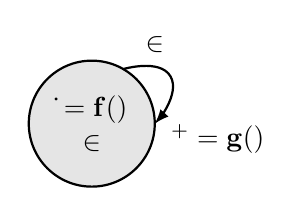
\begin{tikzpicture}
	%
	\fill[gray!20, draw = black,thick] (0,0) circle (0.8cm);
	%	
	\draw (0,0) node[align = center](flow)  {$\dot{\x} = \mathbf{\mathbf{f}}(\x)$\\$\x\in\C$};
	%
	\draw [thick,-latex] plot [smooth, tension=1.2] coordinates { (.4,0.69282) (1,.6) (.8cm,0)};
	%
	\draw (1.6,-0.2) node {$\x^+ = \mathbf{g}(\x)$};
	\draw (.8,1) node {$\x\in\D$};
	%
	\end{tikzpicture}
	\caption[Hybrid automata representiation of the system.]{Hybrid automata: Conceptual representation of the hybrid system $\Ha$ characterized by a single flow map $f$ and one jump map $g$. Only one state and one reset branch are needed to picture the behaviour of the system.}
	\label{fig:HA}
	%\vspace{-5mm}
\end{figure}
%

Let us suppose that the flow map $\mathbf{\mathbf{f}}$ and the jump map $\mathbf{g}$ depend on two sets of \textit{unknown parameters} $\bm{\bm{\alpha}}\in\R^{m_\mathbf{f}}$ and $\bm{\bm{\beta}}\in\R^{m_g}$, i.e.
\[\mathbf{\mathbf{f}} = \mathbf{\mathbf{f}}(\x,\bm{\alpha})\qquad \mathbf{g} = \mathbf{g}(\x,\bm{\beta})\]
and that no \textit{a priori} knowledge of both, the flow set $\C$ and the jump set $\D$ , is available.
Assume that the system is observable, i.e. it is possible to measure and collect samples of the state $\x$.

In order to correctly simulate the system or design a controller for it, it is necessary to identify the parameters in $\bm{\alpha}$, $\bm{\beta}$ and estimate the sets $\C$ and $\D$ from measurements of the state $\x$.

Hereafter, the basic assumptions required to develop the proposed identification method are presented.
Firstly, as a very general hypothesis, both the flow and jump maps are assumed to be linear in the parameters. However, $f$ and $g$ are usually nonlinear with respect to the states.
Thanks to this assumption, it is possible to employ linear identification techniques to estimate the unknown parameters. 
\begin{assum}[Linearity in the parameters]\label{ass:1}
	The maps $f$ and $g$ are linear {with respect to constant} parameters collected in the vectors $\bm{\alpha}\in\R^{m_\mathbf{f}}$ and $\bm{\beta}\in\R^{m_j}$ respectively, i.e., there exist $\bm{\Phi}:\R^{n}\rightarrow\R^{n\times m_f}$ and $\bm{\Psi}:\R^{n}\rightarrow\R^{n\times m_j}$ such that
	\begin{equation*}
	%
	\left\{ 
	\begin{matrix*}[l]\vspace{1pt}
	%
	\dot{\x} = \mathbf{\mathbf{f}}(\x)= \bm{\Phi}(\x)\bm{\alpha}&&\x\in\C\\
	\x^+ = \mathbf{g}(\x)=\bm{\Psi}(\x)\bm{\beta}&&\x\in\D
	%
	\end{matrix*}
	\right.
	%
	\end{equation*}
	{%\color{red} Answer to reviewer \#2 (6)\\
	The maps $\bm{\Phi}$, $\bm{\Psi}$ are assumed to be known a priori.
	} 
\end{assum}
%
The second assumption deals with the regularity of the flow map. %From now on, we denote with $\|\cdot\|$ the 2-norm of a vector.%Another important assumption, is requiring the smoothness and the Lischitzness of the flow map. This will result to be a fundamental hypothesis for the identification procedure. 
\begin{assum}[Smoothness and Lipschitzness of the flow map]\label{ass:2}
The following properties hold for the flow map $\mathbf{\mathbf{f}}$:
\begin{itemize}
	\item[$i)$]  $\mathbf{\mathbf{f}}$ is globally Lipschitz continuous on $\C$, i.e., there exists a constant $k\geq 0$ such that
	\[\forall\x_1,\x_2\in\C\quad\|\mathbf{\mathbf{f}}(\x_1)-\mathbf{\mathbf{f}}(\x_2)\|_2\leq k \|\x_1-\x_2\|_2~. \]
	$k$ is referred as the \textit{Lipschitz constant};
	\item[ii)] $\mathbf{\mathbf{f}}$ is differentiable almost everywhere in $\C$;
	\item[iii)] $\mathbf{\mathbf{f}}$ admits a fixed point in the origin which is inside $\C$, i.e. $\mathbf{\mathbf{f}}(\mymathbb{0}_n)=\mymathbb{0}_n$, $\{\mymathbb{0}_n\}\in\C$.
\end{itemize} 
\end{assum}

\clearpage
%%%%%%%%%%%%%%%%%%%%%%%%%%%%%%%%%%%%%%%%%%%%%%%%%%%%%%%%%%%%%%%%%%%%%%%%%%%%
\section{Jump Detection}\label{JumpD}
%
\begin{defn}[Euler derivative norm]
	Given the hybrid system $(\mathbf{\mathbf{f}},~\mathbf{g},~\C,~\D)$ and a time interval $\delta t>0$, the norm of the Euler derivative of the state is defined as
	\[D_{\delta t}\x(t)= \frac{\|\x(t)-\x(t-\delta t)\|_2}{\delta t}\]
\end{defn}
%
\begin{defn}[Bounded-norm Euler derivative]
	The Euler derivative of a hybrid system $(\mathbf{\mathbf{f}},~\mathbf{g},~\C,~\D)$ has bounded--norm if there exists $\tau(t)\geq 0$ such that
	\[\forall\delta t>0,t\in\R^+~\land~\forall \x\in\C\quad\quad D_{\delta t}\x(t)\leq\tau\]
\end{defn}
%

\begin{thm}[Criteria for the norm bound of the Euler derivative]\label{thm:criteria}
   	%
   	Consider the hybrid system
   	$(\mathbf{\mathbf{f}},~\mathbf{g},~\C,~\D)$. If $\mathbf{\mathbf{f}}(\x)$ satisfies
   	Assumption \ref{ass:2}\footnote{Notice that Assumption \ref{ass:2}($ii$) is
   	not necessary for Theorem \ref{thm:criteria}. However, it will become of fundamental
   	importance later on.} and $\x(t)\in \C ~\forall t \in [t-\delta t,t]$,
   	then the system has bounded--norm Euler derivative with upper bound
	%
	\begin{equation}\label{eq:bound}
		\tau(t)=\frac{1}{\delta t}\int_{t-\delta t}^{t}k\|\x(s)\|_2ds
	\end{equation}
	%
\end{thm}
%
\proof
    %
    Since
    \begin{equation}
        \dot{\x} = \mathbf{\mathbf{f}}(\x)\quad\forall\x\in\C, 
    \end{equation}
    integrating both sides of the equation between $t-\delta t$ and $t$, yields
    %
    \begin{equation}
        \x(t)-\x(t-\delta t) = \int_{t-\delta t}^{t}\mathbf{\mathbf{f}}(\x(s))ds
    \end{equation}
    %
    Therefore,
    %
    \begin{equation}%\label{eq:dtdb}
	    D_{\delta t}\x(t)=\frac{1}{\delta t}\|\x(t)-\x(t-\delta t)\|_2 = \frac{1}{\delta t}\left\lVert\int_{t-\delta t}^{t}\mathbf{\mathbf{f}}(\x(s))ds~\right\rVert_2
    \end{equation}
    %
    Considering the right hand side of the equation, it follows that
    %
    \begin{equation}
        \frac{1}{\delta t}\left\lVert\int_{t-\delta t}^{t}\mathbf{\mathbf{f}}(\x(s))ds~\right\rVert_2\leq\frac{1}{\delta t}\int_{t-\delta t}^{t}\|\mathbf{\mathbf{f}}(\x(s))\|_2ds
    \end{equation}
    %
    Since $f$ is globally Lipschitz in $\C$ and $\mathbf{\mathbf{f}}(\mymathbb{0}_n) = \mymathbb{0}_n$,
    %
    \begin{align}
	    \frac{1}{\delta t}\int_{t-\delta t}^{t}\|\mathbf{\mathbf{f}}(\x(s))\|_2ds &= \frac{1}{\delta t}\int_{t-\delta t}^{t}\|\mathbf{\mathbf{f}}(\x(s))-\mathbf{\mathbf{f}}(\mymathbb{0}_n)\|_2ds\\
	    &\leq\frac{1}{\delta t}\int_{t-\delta t}^{t}k\|\x(s)\|_2ds<\infty
    \end{align}
    %
    where $k$ is the Lipschitz constant. Thus, there exists a $\tau\geq 0$ such that, for all $t$, it holds
    %
    \begin{equation}
        D_{\delta t}\x(t)\leq\frac{1}{\delta t}\int_{t-\delta t}^{t}k\|\x(s)\|_2ds\triangleq\tau(t,\delta t)
    \end{equation}
    The above integral is always limited since, from global Lipschitz continuity of $\mathbf{\mathbf{f}}(\cdot)$, global existence of trajectories $\x(t)$ is assured in $\C$. It follows that on any compact time interval, $[t-\delta t,t]$, where the state does not leave the flow set, the quantity
    %
    \begin{equation}
        \int_{t- \delta t}^{t}\|\x(s)\|_2ds
    \end{equation}
    %
    is limited, providing the result.\\
    %
    $\blacksquare$
    %
\endproof
%
From now on let us refer to $\tau(t)$ as the \textit{smoothness bound}.
%
\begin{exmp}\label{ex:hsid1}
    %
	Consider an hybrid system with the flow described by 
	%
	\begin{equation}
	    \dot{x}={{f}}(x)=\sin(x)\quad x\in\C
	\end{equation}
	%
	where $\C\triangleq[0,2\pi]$. $f$ clearly satisfies Assumption \ref{ass:2} and its Lipschitz constant $k$ can be found as
	%
	\begin{equation}
	    k=\sup\limits_{x\in\C}\left\|\frac{d {f}}{dx}\right\|_2=\sup\limits_{x\in\C}\|\cos(x)\|_2=1
	\end{equation}
	%
	Furthermore, the solution of the ordinary differential equation with $x(0)=x_0$ is\
	%
	\begin{equation}
	    x(t)= 2\tan^{-1}\left(e^{t-\ln(\cot(x_0/2))}\right)
	\end{equation}
	%
	Since ${\mathbf{f}}(0)=0$ ($\{0\}\in\C$) Theorem \ref{thm:criteria} holds and, for any $\delta t>0$ yields
	%
	\begin{equation}\label{eq:exmp_sb}
	    D_{\delta t}x(t)=\frac{1}{\delta t}\|x(t)-x(t-\delta t)\|\leq\frac{1}{\delta t}\int_{t-\delta t}^{t}\|x(s)\|_2ds=\tau(t)
	\end{equation}
	%
	Figure \ref{fig:ex1} shows in a numerical example with $x_0=10^{-2}$ and $\delta t = 0.5$. 
	%
	\begin{figure}[!t]
        \centering
        %
\definecolor{mycolor1}{rgb}{0.00000,0.44706,0.74118}%
%
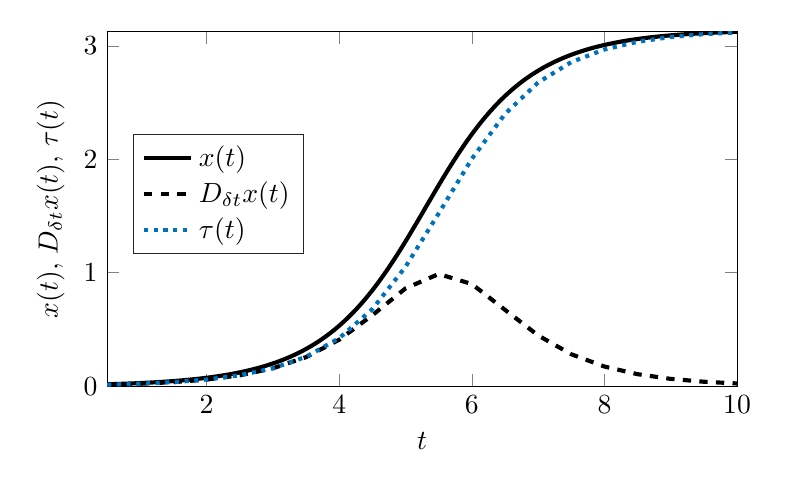
\begin{tikzpicture}

\begin{axis}
[%
width=8cm,
height=4.5cm,
at={(0.614in,0.251in)},
scale only axis,
xmin=0.5,
xmax=10,
ymin=0,
ymax=3.12343333205421,
axis background/.style={fill=white},
xlabel=$t$,ylabel={$x(t),$ $D_{\delta t}x(t)$, $\tau(t)$}, 
legend style={legend cell align=left, align=left, draw=white!15!black, {at={(2.5cm,3.2cm)}}
}
]
\addplot [color=black, line width=1.5pt]
  table[row sep=crcr]{%
0.5	0.0164869766336163\\
0.521939953810624	0.0168526802942833\\
0.543879907621247	0.0172264949765504\\
0.565819861431871	0.0176086005231329\\
0.587759815242494	0.0179991807606994\\
0.609699769053118	0.0183984235878792\\
0.631639722863741	0.0188065210651958\\
0.653579676674365	0.0192236695069702\\
0.675519630484988	0.0196500695752333\\
0.697459584295612	0.0200859263756921\\
0.719399538106236	0.020531449555791\\
0.741339491916859	0.0209868534049148\\
0.763279445727483	0.0214523569567771\\
0.785219399538106	0.0219281840940402\\
0.80715935334873	0.0224145636552135\\
0.829099307159353	0.0229117295438787\\
0.851039260969977	0.0234199208402892\\
0.8729792147806	0.0239393819153934\\
0.894919168591224	0.0244703625473337\\
0.916859122401848	0.0250131180404692\\
0.938799076212471	0.0255679093469781\\
0.960739030023095	0.0261350031910889\\
0.982678983833718	0.0267146721959971\\
1.00461893764434	0.0273071950135207\\
1.02655889145497	0.0279128564565499\\
1.04849884526559	0.0285319476343487\\
1.07043879907621	0.0291647660907644\\
1.09237875288684	0.0298116159454041\\
1.11431870669746	0.0304728080378367\\
1.13625866050808	0.0311486600748806\\
1.15819861431871	0.0318394967810383\\
1.18013856812933	0.0325456500521386\\
1.20207852193995	0.0332674591122494\\
1.22401847575058	0.0340052706739243\\
1.2459584295612	0.0347594391018466\\
1.26789838337182	0.0355303265799362\\
1.28983833718245	0.0363183032819838\\
1.31177829099307	0.037123747545879\\
1.3337182448037	0.0379470460514997\\
1.35565819861432	0.038788594002329\\
1.37759815242494	0.0396487953108679\\
1.39953810623557	0.0405280627879132\\
1.42147806004619	0.0414268183357682\\
1.44341801385681	0.0423454931454554\\
1.46535796766744	0.0432845278980026\\
1.48729792147806	0.0442443729698699\\
1.50923787528868	0.0452254886425893\\
1.53117782909931	0.0462283453166861\\
1.55311778290993	0.0472534237299525\\
1.57505773672055	0.0483012151801435\\
1.59699769053118	0.0493722217521641\\
1.6189376443418	0.0504669565498182\\
1.64087759815242	0.051585943932187\\
1.66281755196305	0.0527297197547054\\
1.68475750577367	0.0538988316150044\\
1.7066974595843	0.0550938391035848\\
1.72863741339492	0.0563153140593882\\
1.75057736720554	0.0575638408303287\\
1.77251732101617	0.0588400165388478\\
1.79445727482679	0.0601444513525529\\
1.81639722863741	0.0614777687599975\\
1.83833718244804	0.062840605851659\\
1.86027713625866	0.0642336136061679\\
1.88221709006928	0.065657457181839\\
1.90415704387991	0.0671128162135495\\
1.92609699769053	0.0686003851150112\\
1.94803695150115	0.0701208733864719\\
1.96997690531178	0.0716750059278844\\
1.9919168591224	0.0732635233575704\\
2.01385681293303	0.0748871823364057\\
2.03579676674365	0.0765467558975437\\
2.05773672055427	0.0782430337816902\\
2.0796766743649	0.0799768227779342\\
2.10161662817552	0.0817489470701315\\
2.12355658198614	0.0835602485888314\\
2.14549653579677	0.0854115873687232\\
2.16743648960739	0.0873038419115765\\
2.18937644341801	0.0892379095546294\\
2.21131639722864	0.0912147068443768\\
2.23325635103926	0.0932351699156896\\
2.25519630484988	0.0953002548761887\\
2.27713625866051	0.0974109381957793\\
2.29907621247113	0.0995682171012352\\
2.32101616628175	0.101773109975709\\
2.34295612009238	0.104026656763022\\
2.364896073903	0.106329919376569\\
2.38683602771363	0.108683982112654\\
2.40877598152425	0.111089952068044\\
2.43071593533487	0.113548959561518\\
2.4526558891455	0.116062158559139\\
2.47459584295612	0.118630727102971\\
2.49653579676674	0.121255867742917\\
2.51847575057737	0.123938807971341\\
2.54041570438799	0.126680800660069\\
2.56235565819861	0.129483124499368\\
2.58429561200924	0.132347084438433\\
2.60623556581986	0.13527401212688\\
2.62817551963049	0.138265266356696\\
2.65011547344111	0.141322233504056\\
2.67205542725173	0.144446327970363\\
2.69399538106236	0.147638992621791\\
2.71593533487298	0.150901699226603\\
2.7378752886836	0.154235948889392\\
2.75981524249423	0.157643272481389\\
2.78175519630485	0.161125231065855\\
2.80369515011547	0.164683416317551\\
2.8256351039261	0.16831945093516\\
2.84757505773672	0.172034989045488\\
2.86951501154734	0.175831716598145\\
2.89145496535797	0.179711351749354\\
2.91339491916859	0.1836756452334\\
2.93533487297921	0.187726380720156\\
2.95727482678984	0.191865375156994\\
2.97921478060046	0.196094479093277\\
3.00115473441109	0.200415576985517\\
3.02309468822171	0.204830587481131\\
3.04503464203233	0.209341463678618\\
3.06697459584296	0.213950193361813\\
3.08891454965358	0.218658799205738\\
3.1108545034642	0.223469338951413\\
3.13279445727483	0.228383905546809\\
3.15473441108545	0.23340462725097\\
3.17667436489607	0.238533667698146\\
3.1986143187067	0.243773225918574\\
3.22055427251732	0.249125536312371\\
3.24249422632794	0.254592868572785\\
3.26443418013857	0.260177527554832\\
3.28637413394919	0.265881853085144\\
3.30831408775982	0.271708219708606\\
3.33025404157044	0.277659036367133\\
3.35219399538106	0.283736746005699\\
3.37413394919169	0.289943825100474\\
3.39607390300231	0.296282783103668\\
3.41801385681293	0.302756161799431\\
3.43995381062356	0.30936653456488\\
3.46189376443418	0.31611650553006\\
3.4838337182448	0.32300870863038\\
3.50577367205543	0.33004580654478\\
3.52771362586605	0.337230489512626\\
3.54965357967667	0.344565474022046\\
3.5715935334873	0.352053501362168\\
3.59353348729792	0.359697336031447\\
3.61547344110854	0.367499763994026\\
3.63741339491917	0.375463590775833\\
3.65935334872979	0.383591639391895\\
3.68129330254042	0.391886748096127\\
3.70323325635104	0.400351767944704\\
3.72517321016166	0.408989560163916\\
3.74711316397229	0.417802993313332\\
3.76905311778291	0.426794940234962\\
3.79099307159353	0.435968274779093\\
3.81293302540416	0.445325868297436\\
3.83487297921478	0.454870585894309\\
3.8568129330254	0.464605282426669\\
3.87875288683603	0.474532798243983\\
3.90069284064665	0.484655954659209\\
3.92263279445728	0.494977549142467\\
3.9445727482679	0.505500350229423\\
3.96651270207852	0.516227092136957\\
3.98845265588915	0.527160469079279\\
4.01039260969977	0.538303129278488\\
4.03233256351039	0.549657668664381\\
4.05427251732102	0.561226624259419\\
4.07621247113164	0.573012467245858\\
4.09815242494226	0.585017595713446\\
4.12009237875289	0.597244327087549\\
4.14203233256351	0.60969489023922\\
4.16397228637413	0.622371417280618\\
4.18591224018476	0.635275935051172\\
4.20785219399538	0.648410356302135\\
4.229792147806	0.661776470589565\\
4.25173210161663	0.675375934888406\\
4.27367205542725	0.689210263943143\\
4.29561200923787	0.703280820373475\\
4.3175519630485	0.717588804556675\\
4.33949191685912	0.732135244311617\\
4.36143187066975	0.746920984413016\\
4.38337182448037	0.761946675968038\\
4.40531177829099	0.777212765691272\\
4.42725173210162	0.792719485117913\\
4.44919168591224	0.808466839798968\\
4.47113163972286	0.824454598526284\\
4.49307159353349	0.840682282639177\\
4.51501154734411	0.857149155468356\\
4.53695150115473	0.873854211976691\\
4.55889145496536	0.890796168659977\\
4.58083140877598	0.90797345377438\\
4.6027713625866	0.925384197960318\\
4.62471131639723	0.943026225335438\\
4.64665127020785	0.96089704513167\\
4.66859122401848	0.978993843953317\\
4.6905311778291	0.997313478734424\\
4.71247113163972	1.01585247047444\\
4.73441108545035	1.03460699883115\\
4.75635103926097	1.05357289764916\\
4.77829099307159	1.07274565150059\\
4.80023094688222	1.09212039331212\\
4.82217090069284	1.11169190314943\\
4.84411085450346	1.13145460822521\\
4.86605080831409	1.15140258419227\\
4.88799076212471	1.17152955777638\\
4.90993071593534	1.19182891079657\\
4.93187066974596	1.21229368561235\\
4.95381062355658	1.23291659202809\\
4.97575057736721	1.25369001567483\\
4.99769053117783	1.27460602787942\\
5.01963048498845	1.29565639701894\\
5.04157043879908	1.31683260134701\\
5.0635103926097	1.33812584326594\\
5.08545034642032	1.35952706500622\\
5.10739030023095	1.3810269656622\\
5.12933025404157	1.40261601952019\\
5.15127020785219	1.42428449560284\\
5.17321016166282	1.44602247834191\\
5.19515011547344	1.46781988928006\\
5.21709006928406	1.48966650969198\\
5.23903002309469	1.5115520040055\\
5.26096997690531	1.53346594389509\\
5.28290993071594	1.5553978329129\\
5.30484988452656	1.57733713151661\\
5.32678983833718	1.59927328234937\\
5.34872979214781	1.62119573562416\\
5.37066974595843	1.64309397446368\\
5.39260969976905	1.66495754004768\\
5.41454965357968	1.6867760564214\\
5.4364896073903	1.70853925482266\\
5.45842956120092	1.73023699739026\\
5.48036951501155	1.75185930012297\\
5.50230946882217	1.77339635496627\\
5.52424942263279	1.79483855091315\\
5.54618937644342	1.8161764940153\\
5.56812933025404	1.83740102621215\\
5.59006928406466	1.85850324289671\\
5.61200923787529	1.87947450914953\\
5.63394919168591	1.9003064745844\\
5.65588914549654	1.9209910867622\\
5.67782909930716	1.941520603142\\
5.69976905311778	1.96188760155069\\
5.72170900692841	1.98208498916477\\
5.74364896073903	2.00210601000943\\
5.76558891454965	2.02194425099092\\
5.78752886836028	2.04159364648878\\
5.8094688221709	2.06104848154354\\
5.83140877598152	2.08030339368453\\
5.85334872979215	2.09935337344974\\
5.87528868360277	2.1181937636565\\
5.8972286374134	2.13682025748759\\
5.91916859122402	2.15522889546172\\
5.94110854503464	2.17341606136161\\
5.96304849884527	2.19137847719531\\
5.98498845265589	2.20911319726849\\
6.00692840646651	2.22661760144651\\
6.02886836027714	2.24388938768539\\
6.05080831408776	2.26092656391023\\
6.07274826789838	2.27772743931873\\
6.09468822170901	2.29429061518559\\
6.11662817551963	2.31061497524142\\
6.13856812933025	2.32669967569721\\
6.16050808314088	2.34254413498228\\
6.1824480369515	2.35814802326026\\
6.20438799076212	2.37351125178428\\
6.22632794457275	2.38863396214847\\
6.24826789838337	2.4035165154892\\
6.270207852194	2.41815948168557\\
6.29214780600462	2.43256362860435\\
6.31408775981524	2.44672991143104\\
6.33602771362587	2.46065946212446\\
6.35796766743649	2.47435357902858\\
6.37990762124711	2.4878137166716\\
6.40184757505774	2.50104147577866\\
6.42378752886836	2.5140385935212\\
6.44572748267898	2.52680693402268\\
6.46766743648961	2.53934847913721\\
6.48960739030023	2.55166531951509\\
6.51154734411085	2.56375964596613\\
6.53348729792148	2.57563374112942\\
6.5554272517321	2.58728997145586\\
6.57736720554272	2.59873077950758\\
6.59930715935335	2.60995867657656\\
6.62124711316397	2.62097623562283\\
6.6431870669746	2.6317860845315\\
6.66512702078522	2.6423908996858\\
6.68706697459584	2.65279339985278\\
6.70900692840647	2.66299634037674\\
6.73094688221709	2.6730025076747\\
6.75288683602771	2.68281471402752\\
6.77482678983834	2.69243579265925\\
6.79676674364896	2.70186859309718\\
6.81870669745958	2.7111159768042\\
6.84064665127021	2.72018081307479\\
6.86258660508083	2.72906597518599\\
6.88452655889146	2.73777433679389\\
6.90646651270208	2.74630876856669\\
6.9284064665127	2.7546721350448\\
6.95034642032333	2.76286729171872\\
6.97228637413395	2.77089708231537\\
6.99422632794457	2.77876433628363\\
7.0161662817552	2.78647186646993\\
7.03810623556582	2.79402246697496\\
7.06004618937644	2.80141891118266\\
7.08198614318707	2.80866394995287\\
7.10392609699769	2.81576030996932\\
7.12586605080831	2.82271069223468\\
7.14780600461894	2.82951777070487\\
7.16974595842956	2.836184191055\\
7.19168591224018	2.84271256956935\\
7.21362586605081	2.84910549214854\\
7.23556581986143	2.85536551342688\\
7.25750577367206	2.86149515599332\\
7.27944572748268	2.86749690970981\\
7.3013856812933	2.8733732311209\\
7.32332563510393	2.87912654294892\\
7.34526558891455	2.88475923366919\\
7.36720554272517	2.89027365716006\\
7.3891454965358	2.89567213242265\\
7.41108545034642	2.9009569433658\\
7.43302540415704	2.90613033865145\\
7.45496535796767	2.91119453159632\\
7.47690531177829	2.91615170012583\\
7.49884526558891	2.92100398677642\\
7.52078521939954	2.92575349874252\\
7.54272517321016	2.93040230796501\\
7.56466512702078	2.93495245125758\\
7.58660508083141	2.9394059304683\\
7.60854503464203	2.94376471267321\\
7.63048498845266	2.94803073039941\\
7.65242494226328	2.95220588187513\\
7.6743648960739	2.95629203130415\\
7.69630484988453	2.96029100916263\\
7.71824480369515	2.964204612516\\
7.74018475750577	2.9680346053541\\
7.7621247113164	2.97178271894256\\
7.78406466512702	2.97545065218887\\
7.80600461893764	2.97904007202137\\
7.82794457274827	2.98255261377968\\
7.84988452655889	2.98598988161526\\
7.87182448036952	2.98935344890064\\
7.89376443418014	2.99264485864618\\
7.91570438799076	2.99586562392321\\
7.93764434180139	2.99901722829245\\
7.95958429561201	3.00210112623681\\
7.98152424942263	3.00511874359753\\
8.00346420323326	3.00807147801295\\
8.02540415704388	3.01096069935902\\
8.0473441108545	3.01378775019087\\
8.06928406466513	3.01655394618481\\
8.09122401847575	3.01926057658004\\
8.11316397228637	3.02190890461966\\
8.135103926097	3.02450016799025\\
8.15704387990762	3.02703557925978\\
8.17898383371825	3.02951632631319\\
8.20092378752887	3.03194357278545\\
8.22286374133949	3.03431845849152\\
8.24480369515012	3.0366420998531\\
8.26674364896074	3.03891559032168\\
8.28868360277136	3.04114000079776\\
8.31062355658199	3.04331638004589\\
8.33256351039261	3.04544575510542\\
8.35450346420323	3.04752913169665\\
8.37644341801386	3.04956749462227\\
8.39838337182448	3.05156180816401\\
8.4203233256351	3.05351301647417\\
8.44226327944573	3.05542204396211\\
8.46420323325635	3.05728979567552\\
8.48614318706698	3.05911715767632\\
8.5080831408776	3.06090499741131\\
8.53002309468822	3.06265416407722\\
8.55196304849885	3.06436548898047\\
8.57390300230947	3.06603978589127\\
8.59584295612009	3.06767785139228\\
8.61778290993072	3.06928046522164\\
8.63972286374134	3.07084839061053\\
8.66166281755196	3.07238237461513\\
8.68360277136259	3.073883148443\\
8.70554272517321	3.07535142777402\\
8.72748267898383	3.07678791307573\\
8.74942263279446	3.07819328991328\\
8.77136258660508	3.07956822925385\\
8.7933025404157	3.08091338776572\\
8.81524249422633	3.08222940811197\\
8.83718244803695	3.0835169192388\\
8.85912240184757	3.08477653665866\\
8.8810623556582	3.08600886272811\\
8.90300230946882	3.08721448692054\\
8.92494226327945	3.08839398609373\\
8.94688221709007	3.08954792475244\\
8.96882217090069	3.09067685530599\\
8.99076212471132	3.09178131832085\\
9.01270207852194	3.09286184276847\\
9.03464203233256	3.09391894626826\\
9.05658198614319	3.09495313532583\\
9.07852193995381	3.09596490556667\\
9.10046189376443	3.09695474196507\\
9.12240184757506	3.09792311906872\\
9.14434180138568	3.09887050121869\\
9.16628175519631	3.09979734276515\\
9.18822170900693	3.10070408827869\\
9.21016166281755	3.10159117275745\\
9.23210161662818	3.1024590218301\\
9.2540415704388	3.10330805195464\\
9.27598152424942	3.10413867061325\\
9.29792147806005	3.10495127650315\\
9.31986143187067	3.10574625972355\\
9.34180138568129	3.10652400195879\\
9.36374133949192	3.10728487665774\\
9.38568129330254	3.10802924920949\\
9.40762124711316	3.10875747711543\\
9.42956120092379	3.10946991015775\\
9.45150115473441	3.11016689056453\\
9.47344110854504	3.1108487531713\\
9.49538106235566	3.1115158255793\\
9.51732101616628	3.11216842831046\\
9.5392609699769	3.11280687495908\\
9.56120092378753	3.11343147234043\\
9.58314087759815	3.11404252063616\\
9.60508083140878	3.11464031353668\\
9.6270207852194	3.11522513838061\\
9.64896073903002	3.11579727629118\\
9.67090069284065	3.11635700230989\\
9.69284064665127	3.11690458552723\\
9.71478060046189	3.11744028921076\\
9.73672055427252	3.11796437093035\\
9.75866050808314	3.11847708268087\\
9.78060046189376	3.11897867100228\\
9.80254041570439	3.11946937709707\\
9.82448036951501	3.11994943694534\\
9.84642032332563	3.12041908141734\\
9.86836027713626	3.12087853638366\\
9.89030023094688	3.12132802282305\\
9.91224018475751	3.12176775692797\\
9.93418013856813	3.12219795020786\\
9.95612009237875	3.12261880959024\\
9.97806004618938	3.12303053751959\\
10	3.12343333205421\\
};
\addlegendentry{$x(t)$}

\addplot [color=black, dashed, line width=1.5pt]
  table[row sep=crcr]{%
0.5	0.0129739532672325\\
1	0.0213887890512713\\
1.5	0.0352567873322842\\
2	0.0580956390510823\\
2.5	0.0956360621103947\\
3	0.157020421985983\\
3.5	0.255987827542454\\
4	0.409638066069622\\
4.5	0.625715552757503\\
5	0.861918250157168\\
5.5	0.98863584781858\\
6	0.899962647892008\\
6.5	0.67261377588965\\
7	0.446772389026869\\
7.5	0.280897000179203\\
8	0.172706018049722\\
8.5	0.105282699117182\\
9	0.0639765998270478\\
9.5	0.0388304878259991\\
10	0.0235578491571697\\
};
\addlegendentry{$D_{\delta t}x(t)$}

\addplot [color=mycolor1, dotted, line width=1.5pt]
  table[row sep=crcr]{%
0.5	0.0129743401088805\\
1	0.0213905225830566\\
1.5	0.0352645543856456\\
2	0.0581304230457569\\
2.5	0.0957916430235894\\
3	0.157713935460563\\
3.5	0.259051089600454\\
4	0.422847086960148\\
4.5	0.679352698203029\\
5	1.05251847669386\\
5.5	1.52300062799024\\
6	2.00392136983382\\
6.5	2.39952510759622\\
7	2.6773929765478\\
7.5	2.85662226418524\\
8	2.96796161927934\\
8.5	3.03610220157572\\
9	3.07756958574395\\
9.5	3.10275178811816\\
10	3.11803248810844\\
};
\addlegendentry{$\tau(t)$}

\end{axis}
\end{tikzpicture}%

        \caption[Example \ref{ex:hsid1}: Time evolution of the state, Euler derivative norm and smoothness bound.]{Example \ref{ex:hsid1}. Time evolution of $x(t)$, $D_{\delta t}x(t)$, $\tau(t)$ for $x_0=10^{-2}$ and $\delta t=0.5$. This figure shows an application example of Theorem \ref{thm:criteria}. Notice that, as predicted by (\ref{eq:exmp_sb}), along the whole trajectory $D_{\delta t}x(t)$ is bounded from above by $\tau(t)$.}
        \label{fig:ex1}
    \end{figure}
    %
\end{exmp}
Thanks to Assumption \ref{ass:2} and the criteria provided by Theorem \ref{thm:criteria}, any jump, i.e. state discontinuities, can be detected from a series of state measurements by inspecting the norm of the Euler derivative. In particular, the system can be considered to be jumping if $D_{\delta t}\x(t)$ is above an empirically estimated \textit{smoothness bound} $\hat{\tau}(t)$
%
{%\color{red} 
and the following assumption is always satisfied.%
\begin{assum}[Discontinuities and sampling time]\label{ass:3}
    For the chosen $\delta t$ and $\hat{\tau}$, it holds:
    \begin{itemize}
        \item[$i)$] $\mathbf{g}(\x)\in\C~~\forall\x\in\D$;
        \item[$ii)$] If there exists a time instant $s\in[t-\delta t,t]$ such that $\x(s)\in\D$, then $s$ is unique; %$\exists ! ~s:~\forall s\in[t-\delta t,t]~~\x(s)\in\D$;
        \item[$iii)$] Let $\x(s)\in\D,~s\in(t-\delta t,t)$. Then,    
        %
        \begin{equation}\label{eq:ass3.3}
            \D_{\delta t} \x(t)\geq \hat{\tau}(t,\delta t).
        \end{equation}
        %
    \end{itemize}
\end{assum}
}
%
It is worth to clarify that Assumption \ref{ass:3}($i$) is needed to ensure that after a jump, the state will go back to the flow set. Moreover,  \ref{ass:3}($ii$) ensures that the sampling time is small enough such that only one jump may happen within one time interval. Finally, \ref{ass:3}($iii$) requires that the sampling time and the estimated smoothness bounds are chose such that a jump can be detected looking at the Euler derivative norm.

% \textcolor{red}{
% Note that (\ref{eq:ass3.3}) becomes
% %
% \begin{align}
%      \D_{\delta t} \x(t) &= \frac{\|\x(t)-\x(t-\delta t)\|_2}{\delta t} =\\
%                          &= \dfrac{1}{\delta t}\left\|\int_s^t\mathbf{\mathbf{f}}(\x(v))dv + \mathbf{g}(\x(s))-\x(t-\delta t)\right\|_2 =\\
%                          &= \dfrac{1}{\delta t}\left\|\int_s^t\mathbf{\mathbf{f}}(\x(v))dv + \mathbf{g}(\x(s))-\x(s) + \int_{t-\delta t}^s\mathbf{\mathbf{f}}(\x(v))dv\right\|_2 = \\
%                          &= \dfrac{1}{\delta t}\left\|\int_s^t\mathbf{\mathbf{f}}(\x(v))dv + \mathbf{g}(\x(s))-\x(s) + \int_{t-\delta t}^s\mathbf{\mathbf{f}}(\x(v))dv\right\|_2
% \end{align}
% %
% and if $g(\x)\neq \x$ it holds
% %
% \begin{equation}
%     \lim_{\delta t\rightarrow 0} \dfrac{1}{\delta t}\left\|\int_s^t\mathbf{\mathbf{f}}(\x(v))dv + \mathbf{g}(\x(s))-\x(t-\delta t)\right\|_2 = \infty
% \end{equation}
% %
% }
%
Therefore, a \textit{jump detection function} can be defined as
%
\begin{equation}
    \gamma(t)\triangleq \left\{ 
        \begin{matrix*}[l]\vspace{1pt}
            %
            0&&\dfrac{1}{\delta t}\|\x(t)-\x(t-\delta t)\|_2 \leq \hat{\tau}(t)\\
            1&&\text{otherwise}
            %
        \end{matrix*}
    \right.
\end{equation}
%	
which is zero during the flows of the system and assumes the value 1 during the jumps.

At any instant of time $\gamma(t)$ allows to determine whether the system is \textit{jumping} of \textit{flowing};
 $\hat{\tau}$ can be adaptively changed as function of the state and/or time.
Note that $\gamma(t)=1$ indicates that the jump just happened and thus the system's state had been inside the jump set $\D$ during the time interval $[t-\delta t,t]$.
%
\begin{rem}
    Assumption \ref{ass:3} ensures two important properties. Firstly, that only one jump is possible between two samples of the state. Secondly, that the discontinuities created by jumps always make the Euler derivative norm to exceed the estimated smoothness bound for the chosen sampling time. 
\end{rem}
%
\clearpage
%%%%%%%%%%%%%%%%%%%%%%%%%%%%%%%%%%%%%%%%%%%%%%%%%%%%%%%%%%%%%%%%%%%%%%%%%%%%%%%%%%%%%
\section{Identification Procedure}\label{Identification}

\subsection{Approximation of the Smoothness Bound}
In order to estimate on-line the smoothness bound (\ref{eq:bound}), it is necessary to approximate the Lipschitz constant $k$ and then numerically integrate the norm of the state between two sampling instants.
At any time instant $t$, the estimated flow map $\hat{\mathbf{f}}(\x,t)$ is defined as
%
\begin{equation}
    \hat{\mathbf{f}}(\x,t)=\bm{\Phi}(\x)\hat{\bm{\alpha}}(t)
\end{equation}
%
where $\hat{\bm{\alpha}}(t)$ is the estimated vector of flow parameters at time $t$. Thanks to Assumption \ref{ass:2}, $\mathbf{f}(\x)$ is differentiable (and so is $\hat{\mathbf{f}}(\x,t)$) and globally Lipschitz on $\C$, the Lipschitz constant will bound from above the supremum of the norm of the Jacobian of $\mathbf{f}(\x)$ in the flow set $\C$:
%
\begin{equation}
    k\geq\sup\limits_{\x\in\C}\left\|\frac{\partial \mathbf{f}(\x)}{\partial\x}\right\|_2.
\end{equation}
%
Since $\mathbf{f}(\x)$ is not known a priori ($\bm{\alpha}$ is unknown), the estimation of $k$ must be carried out employing the estimated flow map $\hat{\mathbf{f}}(\x,t)$. In this paper, as an estimate of the Lipschitz constant, the following quantity is considered:
%
\begin{equation}
    \hat{k} = r\sup\limits_{\x\in\C}\left\|\frac{\partial \hat{\mathbf{f}}(\x,t)}{\partial\x}\right\|_2\quad r>1.
\end{equation}
%
Therefore, the estimated smoothness bound $\hat{\tau}(t)$ is given by
%
\begin{align}
    \hat{\tau}(t) &= \frac{\hat{k}}{\delta t}\int_{t-\delta t}^{t}\|\x(s)\|_2ds =\\
                  &= \frac{r}{\delta t}\sup\limits_{\x\in\C}\left\|\frac{\partial \hat{\mathbf{f}}(\x,t)}{\partial\x}\right\|_2\int_{t-\delta t}^{t}\|\x(s)\|_2ds.
\end{align}
%
Notice that the integral below must be computed numerically. A possible simple choice is to use the first order Newton-Cotes formula (trapezoidal rule). This would yield to the following approximation of $\hat{\tau}(t)$
%
\begin{align}
    \hat{\tau}(t) &=\frac{r}{\delta t}\sup\limits_{\x\in\C}\left\|\frac{\partial \hat{\mathbf{f}}(\x,t)}{\partial\x}\right\|_2\int_{t-\delta t}^{t}\|\x(s)\|_2ds\\
    \label{eq:htau}
                  &\approx\frac{r}{2}\sup\limits_{\x\in\C}\left\|\frac{\partial \hat{\mathbf{f}}(\x,t)}{\partial\x}\right\|_2\big(\|\x(t)\|_2+\|\x(t-\delta t)\|_2\big).
\end{align}
%
It worths to be observed that with this numerical integration algorithm the estimated smoothness threshold does not explicitly depends on $\delta t$.
Other empirical methods for computing the Lipschitz constant of multivariable functions are presented in \cite{mladineo1986algorithm,Wood1996}. Notice that we do not have any \textit{a priori} knowledge of $\C$ and thus, in equation (\ref{eq:htau}) an approximated flow set $\hat{\C}$  should be employed.
%
{%\color{red} \\ Answer to reviewer \#1 (5), reviewer \#2 (7)
\begin{rem}
    The tuning of the multiplicative constant $r$ should be addressed empirically.
    In fact, it has to be chosen considering a trade off between robustness (high $r$ ensures that $\hat{\tau}(t)\geq\tau(t)$ $\forall t$) and accuracy (low $r$ let $\hat{\tau}$ stay below the peaks of $D_{\delta t}\x(t)$ during jumps, i.e. Assumption 3 would be violated).
\end{rem}
}
%
Thus, the final \textit{jump detection function} becomes
%
\begin{equation}
    \gamma(t)\triangleq \left\{ 
        \begin{matrix*}[l]\vspace{1pt}
            %
            0&&\dfrac{1}{\delta t}\|\x(t)-\x(t-\delta t)\|_2 \leq \dfrac{r}{2}\sup\limits_{\x\in\hat{\C}}\left\|\dfrac{\partial \hat{\mathbf{f}}(\x,t)}{\partial\x}\right\|_2\big(\|\x(t)\|_2+\|\x(t-\delta t)\|_2\big)\\
            1&&\text{otherwise}
            %
        \end{matrix*}
    \right.
\end{equation}
%
\subsection{Parameters Estimation}
%{\color{red}DA FARE}\\
Let us assume to observe the system and measure the state $\x$ with a sampling time $\delta t$. Suppose to collect $N_f$ samples during the flows of the system. %and its derivative $\dot{\x}$ 
It holds:
\begin{equation}\label{eq:linflow}
	\begin{bmatrix}\dot{\x}(t_1)\\\dot{\x}(t_2)\\\vdots\\\dot{\x}(t_{N_\mathbf{f}})\end{bmatrix}=
	\begin{bmatrix}\bm{\Phi}(\x(t_1))\\\bm{\Phi}(\x(t_2))\\\vdots\\\bm{\Phi}(\x(t_{N_\mathbf{f}}))\end{bmatrix}\bm{\alpha}
\end{equation}
Similarly, if $N_j$ samples of the states are collected during jumps, i.e., if $\gamma(t_i)=1$ for all $i = 1,\dots,N_j$, yields
\begin{equation}\label{eq:linjump}
	\begin{bmatrix}{\x}(t_1)\\\x(t_2)\\\vdots\\{\x}(t_{N_j})\end{bmatrix}=
	\begin{bmatrix}\bm{\Psi}(\x(t_1-\delta t))\\\bm{\Psi}(\x(t_2-\delta t))\\\vdots\\\bm{\Psi}(\x(t_{N_j}-\delta t))\end{bmatrix}\bm{\beta}
\end{equation}
%Note that, in general, $\delta t$ might not be constant. 
However, in practice, measurements are always affected by noise and, thus, relations (\ref{eq:linflow}) and (\ref{eq:linjump}) do not hold.
In particular, let's assume that an additive noise, $\tilde{\x}(t_i)$, with zero-mean affects the system, i.e., $\x(t_i)=\bar{\x}(t_i)+\tilde{\x}(t_i)$, where $\bar{\x}(t_i)$ is the true value of the state variable.

Thanks to Assumption \ref{ass:1}, the parameters in $\bm{\alpha}$ and $\bm{\beta}$ can be estimated by linear identification techniques. In fact, both equations,  (\ref{eq:linflow}) and (\ref{eq:linjump}) belong to the error-in-variables (EIV) models:
\begin{equation}
	\yb\approx \mathbf{Xa}
\end{equation}
where $\yb = \bar{\yb}+\tilde{\yb}$ is an output's measurements vector and $\mathbf{X} = \bar{\mathbf{X}}+\tilde{\mathbf{X}}$ is an observation matrix, both comprise of a noiseless part ($\bar{\yb}$, $\bar{\mathbf{X}}$), and  a noisy part ($\tilde{\yb}$, $\tilde{\mathbf{X}}$).
%
{%\color{red}\\Ansewer to Reviewer \#1 (2) [Part 1.]\\
In this linear model, the vector of parameters $\mathbf{a}$ could be estimated by mean of a standard linear estimator \cite{ljung1987system}. The choice of the proper estimation scheme should be done considering how the measurement noise is distributed on the possible state--nonlinearities of $\bm{\Phi}$ and $\bm{\Psi}$.
}%with the recursive least squares (RLS) scheme .

The overall identification experiment is carried out as follows: at each sampling time, the jump detection function is computed. If the system is considered to be flowing, the estimated flow parameter $\hat{\bm{\alpha}}$ is updated and the jump parameter $\hat{\bm{\beta}}$ remains unchanged. On the contrary, if a jump state is detected  $\gamma(t)=1$, the jump parameter $\hat{\bm{\beta}}$ will be updated and the flow parameters $\hat{\bm{\alpha}}$ will be unchanged.

Notice that, in order to update the flow parameters $\hat{\bm{\alpha}}$ according to the 
% 
{chosen linear estimation scheme}, the knowledge of the derivative of the state, $\dot{\x}(t)$, is needed. Since we assume to be able of collecting only samples of the state, this quantity has to be computed numerically (Euler derivative, sliding mode, etc.). 
This cumbersome calculation can be avoided by considering that the  linear relation holds even if it is integrated in an interval of time. In fact,  %This might be computed with a simple backward difference or with any finer numerical differentiation techniques. Besides, this step inevitably introduces errors in the system which leads to imperfect estimations even in the noiseless case. In the noisy case, the situation become even worse since the numerical differentiation would amplify the noise. In order to avoid this kind of problems, it can be shown that the linear relation holds even if it integrated in an interval of time. In fact,
%
\begin{align}
	&\dot{\x}(t)=\bm{\Phi}(\x(t))\bm{\alpha}\\
	\Leftrightarrow\quad&\underbrace{\x(t)-\x(t-\delta t)}_{\delta\x(t)} = 
	\underbrace{\int_{t-\delta t}^{t}\bm{\Phi}(\x(s))ds}_{\bm{\bar{\Phi}}(t)}\bm{\alpha}\\\label{eq:intmod}
	\Leftrightarrow\quad&\delta\x(t)={\bm{\bar{\Phi}}}(t)\bm{\alpha}
\end{align}
% 
This propriety has been exploit in the identification experiments by employing the model (\ref{eq:intmod}).
An overview of the procedure used to update the parameters at time $t$ is presented in Algorithm \ref{alg:HID}.
%
%\setlength{\textfloatsep}{2.5pt}
\begin{algorithm}[!b]
    %
	\caption{Identification of the Hybrid System}\label{alg:HID}
	\begin{algorithmic}[1]
		\State \textbf{Input:} $\hat{\bm{\alpha}}(t-\delta t)$, $\hat{\bm{\beta}}(t-\delta t)$, $\x(t)$, $\x(t-\delta t)$
		\State Compute $\hat{\tau}(t)=\dfrac{r}{2}\sup\limits_{\x\in\C}\left\|\dfrac{\partial \hat{\mathbf{f}}(\x,t)}{\partial\x}\right\|_2\big(\|\x(t)\|_2+\|\x(t-\delta t)\|_2\big)$
		\State Compute $\gamma(t)$
		\If {$\gamma(t)=0$}
		%
		\State $\delta\x(t) = \x(t)-\x(t-\delta t)$,~$\bm{\bar{\Phi}}(t)=\int_{t-\delta t}^{t}\bm{\Phi}(\x(s))ds$
		%
		\State Update $\hat{\bm{\alpha}}(t)$ (Linear Estimator)%(RLS)
		\State $\hat{\bm{\beta}}(t)\gets\hat{\bm{\beta}}(t-\delta t)$
		\Else
		%
		\State Update $\hat{\bm{\beta}}(t)$ (Linear Estimator)%(RLS)
		\State $\hat{\bm{\alpha}}(t)\gets\hat{\bm{\alpha}}(t-\delta t)$
		\EndIf
		%
		\State \textbf{Output:} $\hat{\bm{\alpha}}(t)$, $\hat{\bm{\beta}}(t)$
	\end{algorithmic}
\end{algorithm}
%
\subsection{Reduced Order Identification}
Suppose that some parameters in $\bm{\alpha}$ are known before the identification experiment. In particular, without loss of generality, let us assume that all the $m_l$ parameters of the first $l$ components of $\mathbf{f}$ are known. Thus,
%
\begin{equation}
    \bm{\alpha} = \left(\bm{\alpha}_1,\bm{\alpha}_2\right)
\end{equation}
%
where $\bm{\alpha}_1\in\R^{m_l}$ are the known parameters and $\bm{\alpha}_2\in\R^{m_f-m_l}$. In this case, $\bm{\Phi}(\x)$ can be partitioned as
%
\begin{equation}
    \bm{\Phi}(\x) = \begin{bmatrix}\bm{\Phi}_1(\x)&\mathbb{O}_{l\times (m_f-m_l)}\\\mathbb{O}_{(n-l)\times m_l}&\bm{\Phi}_2(\x)\end{bmatrix}
\end{equation}
%
with $\bm{\Phi}_1(\x)\in\R^{l\times m_l}$ and $\bm{\Phi}_2(\x)\in\R^{(n-l)\times (m_f-m_l)}$.
Therefore, the identification experiment should be applied only to the subsystem
\begin{equation}\label{eq:redflow}
\dot{\x}_2=\bm{\Phi}_2(\x)\bm{\alpha}_2
\end{equation}
This is justified in many physical systems described by a set of second order differential equations (see Example \ref{ex:ex2}).

Notice that the same situation might happen for a jump map. In this case, 
%
\begin{equation}
    \bm{\Psi}(\x) = \begin{bmatrix}\bm{\Psi}_1(\x)&\mathbb{O}_{l\times (m_j-m_l)}\\\mathbb{O}_{(n-l)\times m_l}&\bm{\Psi}_2(\x)\end{bmatrix},\quad\bm{\beta} = \left(\bm{\beta}_1,\bm{\beta}_2\right)
\end{equation}
%
and the model considered for the identification would be
%
\begin{equation}
    \label{eq:redjump}{\x}^+_2=\bm{\Psi}_2(\x)\bm{\beta}_2
\end{equation}
%
Similarly, if $\bm{\Phi}(\x)$ can be partitioned as
%
\begin{equation}
    \bm{\Phi}(\x) = \begin{bmatrix}\bm{\Phi}_1(\x)&\bm{\Phi}_2(\x)\end{bmatrix}
\end{equation}
%
and the first $m_l$ parameters are known, the identification problem can be set up as
%
\begin{equation}
    \dot{\x}-\bm{\Phi}_1(\x)\bm{\alpha}_1=\bm{\Phi}_2(\x)\bm{\alpha}_2
\end{equation}
%
In the same way, for a jump, if 
%
\begin{equation}
    \bm{\Psi}(\x) = \begin{bmatrix}\bm{\Psi}_1(\x)&\bm{\Psi}_2(\x)\end{bmatrix}
\end{equation}
%
the linear model for the identification experiment would result to be
%
\begin{equation}
    {\x}^+-\bm{\Psi}_1(\x)\bm{\beta}_1=\bm{\Psi}_2(\x)\bm{\beta}_2
\end{equation}
%
This approach is justified when, for some components of $\mathbf{f}$ or $\mathbf{g}$, the parameters vector is partially known (see Example \ref{ex:ex3}).
%
\begin{exmp}\label{ex:ex2}
	Let the flow of the hybrid system be described by the following differential equation
	%
	\begin{equation}
	    \ddot{z}=a\dot{z}+b\sin(z)
	\end{equation}
	%
	Define $\x = [x_1,x_2]^\top=[z,\dot{z}]^\top$. The canonical first order state--space equation becomes
	\[\dot{\x}=\begin{bmatrix}x_2\\ax_2+b\sin(x_1)\end{bmatrix}=\begin{bmatrix}x_2&0&0\\0&x_2&\sin(x_1)\end{bmatrix}\begin{bmatrix}1\\a\\b\end{bmatrix}\]
	It is clear that we are interested only in the parameters $a$ and $b$. Therefore it is convenient to consider only the subsystem
	\[\dot{x}_2=\begin{bmatrix}x_2&\sin(x_1)\end{bmatrix}\begin{bmatrix}a\\b\end{bmatrix}\] 
	in the identification experiment.
\end{exmp}
%\iffalse 
\begin{exmp}\label{ex:ex3}
	Let $\x=[x_1,x_2]^\top$ and consider the following jump map
	%
	\begin{align}
	    {\x}^+=\begin{bmatrix}x_1+cx_2^2\\a\|x_2\|_2+b\sin(x_1)\end{bmatrix}=
	    =\begin{bmatrix}x_1&x_2^2&0&0\\0&0&\|x_2\|_2&\sin(x_1)\end{bmatrix}\begin{bmatrix}1\\c\\a\\b\end{bmatrix}
	\end{align}
	Then, during the Identification experiment it is worth considering only the linear relation
	%
	\begin{equation}
	    {\x}^+-\begin{bmatrix}x_1\\0\end{bmatrix}=\begin{bmatrix}x_2^2&0&0\\0&\|x_2\|_2&\sin(x_1)\end{bmatrix}\begin{bmatrix}c\\a\\b\end{bmatrix}
	\end{equation}
	%
\end{exmp}
%\fi 
%
%\vspace{-8mm}
\subsection{Flow and Jump Sets Approximation}
The method to approximate the flow and jump sets proposed in this paper is developed from the following idea. Since it is possible to determine the ``state" of the system, i.e.  whether the system is flowing or it has jumped, it is possible to subdivide the samples of the state in two different sets, a set $\Lambda$ containing the state's samples during flows and a set $\Gamma$ containing the state's samples corresponding to jumps. Then, the approximated flow set $\hat{\C}$ and jump set $\hat{\D}$ are obtained by computing the convex hull of $\Lambda$ and $\Gamma$ respectively. The detailed procedure is reported in Algorithm \ref{alg:m}.%\footnote{The expression $\conv(\cdot)$ refers to the convex hull of the points contained in the set $\cdot$.}. 
{%\color{red}\\Answer to Reviewer \#1 (1)
\begin{rem}
In case $\C$ and $\D$ are assumed convex sets, the approximation results offer an accurate representations of them, consistent with the regions explored by the state of the system. Otherwise, $\hat{\C}$ and $\hat{\D}$ will be a redundant representation of the flow and jump sets. In this case, other techniques might be implemented for a better approximation, e.g. machine--learning--related methods. However, these further investigations fall out of the scope of this paper and will be treated in future work.
\end{rem}
}
%{\color{red} Forse la parte seguente e' meglio metterla nelle conclusioni...Notice that the main drawback of this method is the need of storing all the data points during the identification experiment, leading to memory problems.}%Once a new sample of the state is available and the function $\gamma(t)$ has been computed, the state sample is stored in a set $\Lambda$ if the system 
\begin{algorithm}[!t]
	\caption{Approximation of the flow and jump sets}\label{alg:m}
	\begin{algorithmic}[1]
		\State \textbf{Input:} $\hat{\bm{\alpha}}(t-\delta t)$, $\x(t)$, $\x(t-\delta t)$, $\Lambda(t-\delta t)$, $\Gamma(t-\delta t)$
		\State Compute $\hat{\tau}(t)=\dfrac{r}{2}\sup\limits_{\x\in\hat{\C}}\|\dfrac{\partial \hat{\mathbf{f}}_t}{\partial\x}\|\left[\|\x(t)\|+\|\x(t-\delta t)\|\right]$
		\State Compute $\gamma(t)$
		\If {$\gamma(t)=0$}
		\State $\Lambda(t)\gets\Lambda(t-\delta t)\cup\{\x(t)\}$
		\State $\Gamma(t)\gets\Gamma(t-\delta t)$
		\Else
		\State $\Lambda(t)\gets\Lambda(t-\delta t)\cup\{\x(t)\}\backslash\{\x(t-\delta t)\}$
		%\State $\Lambda(t)\gets\Lambda(t-\delta t)\backslash\{\x(t-\delta t)\}$
		\State $\Gamma(t)\gets\Gamma(t-\delta t)\cup\{\x(t-\delta t)\}$
		\EndIf
		\State $\hat{\C}(t) = \conv(\Lambda(t))$
        \State $\hat{\D}(t)=\conv(\Gamma(t))$
		\State \textbf{Output:} $\hat{\C}(t)$, $\hat{\D}(t)$, $\Lambda(t)$, $\Gamma(t)$
		\vspace{-5mm}
	\end{algorithmic}
	\vspace{5mm}
	%\ignorespacesafterend
\end{algorithm}

\clearpage
%%%%%%%%%%%%%%%%%%%%%%%%%%%%%%%%%%%%%%%%%%%%%%%%%%%%%%%%%%%%%%%%%%%%%%%%%%%%%%%%%%%%%
\section{Simulation Experiments}\label{Experiments}
\subsection{Case of Study: Impact Mass-Spring-Damper System}
Let us consider an impact mass-spring-damper system represented in Fig. \ref{fig:msd} and let $q$ be height from the ground of the mass. Assume the mass to be unitary and the rest position of the spring to be at the origin ($q=0$). The choice of this system is motivated by the fact that it admits a hybrid port--Hamiltonian representation. In fact, we want to show that the developed identification procedure can be applied to the class of systems with which this Thesis is dealing.
%
\begin{figure}[!b]
	\centering
	\begin{tikzpicture}[scale=1.1, every node/.style={scale=1}]
\tikzstyle{spring}=[thick,decorate,decoration={zigzag,pre length=0.3cm,post length=0.3cm,segment length=6}]
\tikzstyle{damper}=[thick,decoration={markings,  
  mark connection node=dmp,
  mark=at position 0.5 with 
  {
    \node (dmp) [thick,inner sep=0pt,transform shape,rotate=-90,minimum width=15pt,minimum height=3pt,draw=none] {};
    \draw [thick] ($(dmp.north east)+(2pt,0)$) -- (dmp.south east) -- (dmp.south west) -- ($(dmp.north west)+(2pt,0)$);
    \draw [thick] ($(dmp.north)+(0,-5pt)$) -- ($(dmp.north)+(0,5pt)$);
  }
}, decorate]
\tikzstyle{ground}=[fill,pattern=north east lines,draw=none,minimum width=0.75cm,minimum height=0.3cm,inner sep=0pt,outer sep=0pt]

\node [draw, outer sep=0pt, thick, fill = gray!25] (M) [minimum width=2cm, minimum height=1cm] {$m$};

\node (ground) [ground,anchor=north,yshift=-0.2cm,minimum width=5cm,xshift=0.8cm] at (M.south) {};
\draw (ground.north west) -- (ground.north east);
\draw (ground.south east) -- (ground.south west);

\node (fill) [ground,xshift=-0.15cm,minimum height = 0.3cm, minimum width = 0.3cm] at (ground.west) {};
\draw (fill.north west) -- (fill.south west) -- (fill.south east);

\draw [thick, fill = gray] (M.south west) ++(0.2cm,-0.125cm) circle (0.125cm)  (M.south east) ++(-0.2cm,-0.125cm) circle (0.125cm);

\node (wall) [ground, rotate=-90, minimum width=2cm,anchor=south east] at (fill.north west) {};
\draw (wall.north east) -- (wall.north west) -- (wall.south west) -- (wall.south east);

\node (fill2) [ground,xshift=0.15cm,minimum height = 0.3cm, minimum width = 0.3cm] at (ground.east) {};
\draw (fill2.north east) -- (fill2.south east) -- (fill2.south west);
\node (wall2) [ground, rotate=-90, minimum width=1.2cm,anchor=south east] at (fill2.north west) {};
\draw (wall2.north east) -- (wall2.north west) -- (wall2.south west) -- (wall2.south east);

\draw [-,thick] (M.west) -- +(-0.4cm,0) node [name = t] {};
\draw [-,ultra thick] (t.north) -- (t.south);
\draw [spring] (M.15) -- node [xshift=0.3cm,yshift=0.195cm] {$a$} ++(2.1cm,0cm);
\draw [damper] (M.345) -- node [xshift=0.3cm,yshift=-0.175cm] {$b$} ++(2.1cm,0cm);

\draw [-latex,very thick] (wall.north west) ++(0cm, -0.05cm) -- +(5cm,0cm);
\draw [dotted, thick] (t.north) -- node [yshift=0.85cm] (y1) {$q$} +(0cm,1.4cm);

\end{tikzpicture} 

    \caption[Impact mass--spring--damper system.]{Impact mass--spring--damper system. $q$ is the distance of the cart from the wall, $m$ is the mass of the cart, $a$ is the spring stiffness and $b$ the damping coefficient of the dashpot.} 
    \label{fig:imsd}
\end{figure}
%
\subsubsection{Model of the Flows}
%
When the ball is not touching the floor, the system behaves as a simple damped linear oscillator. Let $\x = [x_1,x_2]^\top = [q,\dot{q}]^\top$. The flows of the system are described by 
\begin{align}
	\dot{\x}&=\begin{bmatrix}x_2\\-ax_1-bx_2\end{bmatrix}
	=\begin{bmatrix}x_2&0&0\\0&-x_1&-x_2\end{bmatrix}\begin{bmatrix}1\\a\\b\end{bmatrix}
\end{align}
%
{where $a$ and $b$ are the spring stiffness and the damping coefficient, respectively}. The corresponding flow set flow set is
%
\begin{equation}
    \C = \{\x:x_1\geq0\}\setminus\{\x:x_1=0,x_2<0\}
\end{equation}
%
\subsubsection{Model of the Jumps}
%
It is clear that during the collision between ball and the floor ($x_1 = q =0$) there is a discontinuity in the velocity. In this example, collisions are considered partially inelastic while the ball is modeled as a rigid body. The selected jump map to model the collisions is the following:
%
\begin{align}
	\x^+=\begin{bmatrix}x_1\\-\lambda x_2+\mu\end{bmatrix} = \begin{bmatrix}x_1&0&0\\0&-x_2&1\end{bmatrix}\begin{bmatrix}1\\\lambda\\\mu\end{bmatrix}
\end{align}
%
{where $\lambda$ is the restitution coefficient and $\mu$ is introduced to consider possible unmodeled impact dynamics}. The jump set is therefore,
%
\begin{equation}
    \D=\{\x:x_1=0,x_2\leq 0\}
\end{equation}
%
\begin{rem}[Hybrid port--Hamiltonian formulation]
    \textcolor{red}{NOTE: the formal definition of hybrid port--Hamiltonian systems will be provided in Chapter 3 in the next version of the Thesis.}
    
    Let $p\triangleq\dot{q}$. The hybrid port--Hamiltonian formulation of the impact mass--spring--damper system is
    %
    \begin{equation}
        \left\{
            \begin{matrix*}[l]
                \begin{bmatrix}\dot{q}\\\dot{p}\end{bmatrix} = \begin{bmatrix}0&1\\-1&-b\end{bmatrix}\begin{bmatrix}\nabla_q\Ha(q,p)\\\nabla_p\Ha(q,p)\end{bmatrix} + \begin{bmatrix}0\\1\end{bmatrix}u & (q,p)\in\C\\
                \begin{bmatrix}q^+\\{p}^+\end{bmatrix} =\begin{bmatrix}q\\-\lambda p+\mu\end{bmatrix}  & (q,p)\in\D\\
                y = p
            \end{matrix*}
        \right.
    \end{equation}
    %
    with 
    %
    \begin{equation}
        \Ha(q,p) \triangleq \frac{1}{2}p^2 + \frac{a}{2}q^2
    \end{equation}
    %
    Note that, if $\mu\leq 0$, the system is \textit{flow passive}.
\end{rem}
%
\subsubsection{Model Identification}
In order to estimate the system's parameters, a reduced order identification has to be performed for both the flow and the jump as in (\ref{eq:redflow}) and (\ref{eq:redjump}). Let $\bm{\alpha} = \left[{\alpha}_1,{\alpha}_2\right]^\top=\left[a,b\right]^\top$ and $\bm{\beta} = \left[{\beta}_1,{\beta}_2\right]^\top = [\lambda,\mu]^\top$
The reduced model for the flow is
%
\begin{equation}
    \dot{\x}_2 = \begin{bmatrix}-x_1&-x_2\end{bmatrix}\begin{bmatrix}{\alpha}_1\\{\alpha}_2\end{bmatrix}
\end{equation}
%
and the one for the jump is
%
\begin{equation}
    \x_2^+ = \begin{bmatrix}-x_2&1\end{bmatrix}\begin{bmatrix}{\beta}_1\\{\beta}_2\end{bmatrix}
\end{equation}
%
The approximation of the  smoothness bound can be derived by computing the supremum of the norm of the estimated flow map Jacobian. Hence, the estimated flow map in the reduced model will be
%
\begin{equation}
    \hat{{f}}(\x,t)=-\hat{{\alpha}}_1(t)x_1(t)-\hat{{\alpha}}_2(t)x_2(t) = -\bm{\alpha}^\top\x
\end{equation}
%
Therefore,
\begin{align*}
	\frac{\partial \hat{{f}}(\x,t)}{\partial \x} = -\hat{\bm{\alpha}}(t)
	\Rightarrow\sup\limits_{\x\in\hat{\C}}\left\|\frac{\partial \hat{{f}}(\x,t)}{\partial\x}\right\|_2 = \left\|\hat{\bm{\alpha}}(t)\right\|_2
\end{align*}
%
\subsection{Numerical Simulation}
To validate the proposed identification method, numerical simulations have been performed. The simulation experiments have been carried out using Hybrid Equations (HyEQ) Toolbox \cite{sanfelice2013toolbox} for the MATLAB environment. The parameters of the system have been chosen as $a = 5$, $b = 0.1$, $\lambda=0.99$, $\mu=0$. 
%
The initial condition and the time span of the simulation have been set to $\x(t_0)=[20,0]^\top$ and $20$ seconds, respectively. Furthermore, the sampling time $\delta t$ has been chosen to be $0.5\cdot 10^{-3}$ s, the multiplicative constant $r$ in the smoothness bound has been set to 220 and the estimated smoothness bound has been initialized to $10^5$.

Here, as both the flow and jump maps result linear in the state, the chosen estimation scheme is the \textit{recursive least squares} (RLS) \cite{ljung1987system}. However, due to how noise would influence the system, i.e. it affects the observation matrix, alternative results might be achieved with a \textit{recursive generalized total least squares} \citep{RHODE20144637} or a \textit{recursive Frisch scheme} (see [c1,c2]). The resulting time evolution of the system is represented in Fig. \ref{fig:trj}. 
\begin{figure}
	\centering
%	\includegraphics[trim={15 0 0 0},scale=.58]{trj}
    % This file was created by matlab2tikz.
%
%The latest updates can be retrieved from
%  http://www.mathworks.com/matlabcentral/fileexchange/22022-matlab2tikz-matlab2tikz
%where you can also make suggestions and rate matlab2tikz.
%
\definecolor{mycolor1}{rgb}{0.00000,0.44700,0.74100}%
%
\begin{tikzpicture}
%\footnotesize

\begin{axis}[%
width=9cm,
height=2.5cm,
at={(0.86in,2.2in)},
scale only axis,
xmin=0,
xmax=20,
ymin=-2.665645482125e-12,
ymax=20,
ylabel style={font=\color{white!15!black}},
ylabel={$x_1(t) = q(t)$},
axis background/.style={fill=white},
legend style={legend cell align=left, align=left, draw=white!15!black}
]
\addplot [color=black, line width=1.5pt]
  table[row sep=crcr]{%
0	20\\
0	20\\
0.000126191468896039	19.999999203789\\
0.000252382937792077	19.9999968151695\\
0.000378574406688116	19.9999928341618\\
0.000504765875584155	19.9999872607862\\
0.00113572322006435	19.9999355091145\\
0.00176668056454454	19.9998439513818\\
0.00239763790902473	19.9997125902819\\
0.00302859525350493	19.9995414285877\\
0.00618338197590589	19.9980887137718\\
0.00933816869830686	19.9956414454642\\
0.0124929554207078	19.992200059144\\
0.0156477421431088	19.9877650395981\\
0.0276481601076166	19.9618263167084\\
0.0396485780721244	19.9215546749277\\
0.0516489960366322	19.866996276571\\
0.06364941400114	19.7982075093252\\
0.0795171060289317	19.6855171395325\\
0.0953847980567235	19.5482452791905\\
0.111252490084515	19.3866035496145\\
0.127120182112307	19.2008338295377\\
0.145352130059267	18.95795008083\\
0.163584078006226	18.6840334854967\\
0.181816025953186	18.3795953849762\\
0.200047973900146	18.0451965342848\\
0.220071234980976	17.6441482118668\\
0.240094496061806	17.2085733293003\\
0.260117757142636	16.7394132942873\\
0.280141018223465	16.237673951143\\
0.301708193087325	15.6620310918154\\
0.323275367951185	15.0512499408405\\
0.344842542815045	14.4068253719306\\
0.366409717678905	13.7303252164943\\
0.389458650570211	12.973744025447\\
0.412507583461517	12.1844913788867\\
0.435556516352823	11.3647370424498\\
0.458605449244129	10.5167230979711\\
0.481800361400667	9.63714868602161\\
0.504995273557205	8.73372514967301\\
0.528190185713743	7.80893592384127\\
0.551385097870281	6.86531151233252\\
0.572725339283812	5.9827171210837\\
0.594065580697343	5.0883994583547\\
0.615405822110874	4.1844184005378\\
0.636746063524405	3.27284792754387\\
0.655724669033981	2.45746986002715\\
0.674703274543557	1.63921747342536\\
0.693681880053134	0.819568951208989\\
0.71266048556271	-1.16795462190566e-13\\
};
%egendentry{data1}

\addplot [color=black, line width=1.5pt]
  table[row sep=crcr]{%
0.71266048556271	-1.16795462190566e-13\\
0.71266048556271	-1.16795462190566e-13\\
0.712955847869028	0.0126189596129195\\
0.713251210175347	0.0252375410107193\\
0.713546572481665	0.0378557387003791\\
0.713841934787984	0.0504735471893269\\
0.715318746319577	0.113556559409491\\
0.716795557851169	0.176629017917934\\
0.718272369382762	0.23969023652624\\
0.719749180914355	0.302739529275859\\
0.727133238572319	0.61778312183889\\
0.734517296230282	0.932425810234085\\
0.741901353888246	1.24658213969462\\
0.74928541154621	1.56016686985453\\
0.763502620608957	2.16201786746632\\
0.777719829671705	2.76083038101713\\
0.791937038734452	3.35600386151082\\
0.8061542477972	3.94694278678755\\
0.823290826869658	4.65275954696095\\
0.840427405942117	5.35054247500561\\
0.857563985014576	6.03928135536863\\
0.874700564087035	6.71798222602084\\
0.893860482784055	7.46373027842436\\
0.913020401481075	8.19436575900548\\
0.932180320178095	8.90857727943182\\
0.951340238875115	9.60508820806833\\
0.972141894914274	10.3397948501332\\
0.992943550953433	11.0506307160876\\
1.01374520699259	11.7361083120558\\
1.03454686303175	12.3948010671445\\
1.05684159758016	13.0694840401591\\
1.07913633212858	13.7102252456922\\
1.10143106667699	14.3155085611607\\
1.12372580122541	14.8839131350341\\
1.14740771745168	15.4458111627729\\
1.17108963367795	15.96312788429\\
1.19477154990422	16.4345184665667\\
1.21845346613049	16.858774356195\\
1.24035979590319	17.2083202759852\\
1.26226612567589	17.5158640540576\\
1.28417245544859	17.7807597207985\\
1.30607878522129	18.0024671767266\\
1.32593990787618	18.1657806399565\\
1.34580103053108	18.2929826286987\\
1.36566215318598	18.3838938163702\\
1.38552327584088	18.4384075932583\\
1.40289087903558	18.4562184192618\\
1.42025848223028	18.4461909090966\\
1.43762608542497	18.4083883711415\\
1.45499368861967	18.3429160315414\\
1.47007626831375	18.2637219725677\\
1.48515884800783	18.1638913797042\\
1.50024142770191	18.0435687955398\\
1.51532400739599	17.9029218056077\\
1.53303076113948	17.7121261385877\\
1.55073751488298	17.4939299726845\\
1.56844426862648	17.2487235048843\\
1.58615102236997	16.9769383256841\\
1.60575291074699	16.6456381807801\\
1.62535479912401	16.2830444129758\\
1.64495668750104	15.8899142399392\\
1.66455857587806	15.4670613128123\\
1.68574693571507	14.9775614103505\\
1.70693529555209	14.4555193598167\\
1.72812365538911	13.9021747809028\\
1.74931201522613	13.3188333200789\\
1.77198263544398	12.6630191231148\\
1.79465325566183	11.9761935150489\\
1.81732387587968	11.2601900901953\\
1.83999449609754	10.51691029426\\
1.86363936925682	9.71475515600215\\
1.8872842424161	8.88737755918985\\
1.91092911557539	8.03714789951455\\
1.93457398873467	7.16649034677414\\
1.95640703129971	6.34655047407202\\
1.97824007386476	5.51329289591894\\
2.0000731164298	4.66873114009761\\
2.02190615899484	3.81489774912013\\
2.04168484028799	3.03511556783754\\
2.06146352158114	2.25094501071307\\
2.08124220287429	1.46392753245248\\
2.10102088416744	0.675604766545745\\
2.1052593564867	0.506649350587227\\
2.10949782880595	0.337719947961567\\
2.11373630112521	0.168831768713831\\
2.11797477344446	-4.82169859594705e-13\\
};
%%egendentry{data2}

\addplot [color=mycolor1, dotted, line width=1.0pt, mark size=1.5pt, mark=asterisk, mark options={solid, fill=gray, gray}]
  table[row sep=crcr]{%
0.71266048556271	-1.16795462190566e-13\\
0.71266048556271	-1.16795462190566e-13\\
};
%%egendentry{data3}

\addplot [color=black, line width=1.5pt]
  table[row sep=crcr]{%
2.11797477344446	-4.82169859594705e-13\\
2.11797477344446	-4.82169859594705e-13\\
2.11829483681149	0.0126189438676957\\
2.11861490017851	0.0252374773928329\\
2.11893496354553	0.0378555941248824\\
2.11925502691256	0.0504732876142727\\
2.12085534374767	0.113555180719346\\
2.12245566058279	0.176625525564236\\
2.12405597741791	0.239683516439594\\
2.12565629425302	0.302728347931474\\
2.1336578784286	0.617726958449652\\
2.14165946260418	0.932275947496817\\
2.14966104677976	1.24627501393359\\
2.15766263095534	1.55962413873017\\
2.17210867042261	2.12337793240863\\
2.18655470988987	2.68410395597894\\
2.20100074935714	3.2412218095027\\
2.2154467888244	3.79415619120717\\
2.23272736833193	4.44929241107515\\
2.25000794783947	5.09666054369097\\
2.267288527347	5.73530798034574\\
2.28456910685454	6.36429797353247\\
2.30383919311945	7.0531874106365\\
2.32310927938437	7.72766924076261\\
2.34237936564929	8.3865196245531\\
2.36164945191421	9.02854808964311\\
2.38254650666801	9.70442718987452\\
2.40344356142182	10.3577316893883\\
2.42434061617562	10.9870830275905\\
2.44523767092943	11.5911606095607\\
2.46762420449579	12.2088220852721\\
2.49001073806216	12.7945494794438\\
2.51239727162852	13.3469471350779\\
2.53478380519489	13.8647095567399\\
2.55835704859259	14.3711445958366\\
2.58193029199029	14.8365125733303\\
2.605503535388	15.2596174719699\\
2.6290767787857	15.6393873492776\\
2.65086589188565	15.9510499404283\\
2.6726550049856	16.2242174850569\\
2.69444411808555	16.4583253530246\\
2.7162332311855	16.6529047294774\\
2.73596748835466	16.7947067725888\\
2.75570174552381	16.9035639683676\\
2.77543600269296	16.9793292090018\\
2.79517025986212	17.021920787247\\
2.81236092130652	17.0319722525132\\
2.82955158275092	17.0168648274309\\
2.84674224419532	16.9766639367958\\
2.86393290563973	16.9114720789629\\
2.87922900288253	16.8325654993826\\
2.89452510012534	16.7341048964339\\
2.90982119736815	16.6162352312511\\
2.92511729461096	16.4791238986312\\
2.94296722918862	16.2950460002234\\
2.96081716376628	16.0853634408954\\
2.97866709834395	15.8504556056461\\
2.99651703292161	15.5907411291298\\
3.01623241430944	15.2756050051674\\
3.03594779569726	14.9314360295398\\
3.05566317708508	14.5589596304773\\
3.07537855847291	14.1589540890403\\
3.09666795646215	13.6970577871726\\
3.1179573544514	13.2051430042799\\
3.13924675244064	12.684387304839\\
3.16053615042989	12.1360295489024\\
3.18330666981761	11.5204444463421\\
3.20607718920533	10.8764342161001\\
3.22884770859305	10.2057315609182\\
3.25161822798078	9.51013158989316\\
3.27514370847273	8.76729041346104\\
3.29866918896469	8.00196885247963\\
3.32219466945665	7.21633572663269\\
3.34572014994861	6.41260685692784\\
3.36742412118392	5.65701299033144\\
3.38912809241923	4.8897512078299\\
3.41083206365454	4.11265258341808\\
3.43253603488985	3.32756419890733\\
3.45217379031709	2.61188482538239\\
3.47181154574433	1.89257956998755\\
3.49144930117157	1.17104158251362\\
3.51108705659881	0.448663490638958\\
3.5141375591335	0.336464603605832\\
3.5171880616682	0.224284239220132\\
3.52023856420289	0.112127629383403\\
3.52328906673759	-3.96016552883793e-13\\
};
%%egendentry{data4}

\addplot [color=mycolor1, dotted, line width=1.0pt, mark size=1.5pt, mark=asterisk, mark options={solid, fill=gray, gray}]
  table[row sep=crcr]{%
2.11797477344446	-4.82169859594705e-13\\
2.11797477344446	-4.82169859594705e-13\\
};
%%egendentry{data5}

\addplot [color=black, line width=1.5pt]
  table[row sep=crcr]{%
3.52328906673759	-3.96016552883793e-13\\
3.52328906673759	-3.96016552883793e-13\\
3.5236358969078	0.0126189267917385\\
3.52398272707801	0.0252374083394138\\
3.52432955724823	0.0378554370687596\\
3.52467638741844	0.0504730054063961\\
3.52641053826951	0.113553676195286\\
3.52814468912058	0.176621701501812\\
3.52987883997164	0.239676135282758\\
3.53161299082271	0.302716031874665\\
3.54028374507805	0.617664402776339\\
3.54895449933339	0.932107720218401\\
3.55762525358872	1.24592826321028\\
3.56629600784406	1.55900868254307\\
3.58097438776973	2.08699546246245\\
3.59565276769541	2.6119612655599\\
3.61033114762108	3.13334529646683\\
3.62500952754675	3.6505919358197\\
3.64243895355396	4.25864973450544\\
3.65986837956118	4.85918623300984\\
3.67729780556839	5.45130288842576\\
3.69472723157561	6.03411666155787\\
3.71411224299136	6.67033896614796\\
3.73349725440711	7.29280991655066\\
3.75288226582286	7.90038725949764\\
3.77226727723862	8.49196082121752\\
3.79326454803279	9.11343117156367\\
3.81426181882696	9.71353220481969\\
3.83525908962113	10.2909865656314\\
3.8562563604153	10.8445721205768\\
3.87873997832658	11.409558589341\\
3.90122359623787	11.9444754847071\\
3.92370721414915	12.4480388775823\\
3.94619083206043	12.9190502630116\\
3.96964932183274	13.3745814015142\\
3.99310781160505	13.7922958010649\\
4.01656630137735	14.1711329917699\\
4.04002479114966	14.5101453521836\\
4.06168911755179	14.7871310853299\\
4.08335344395393	15.0288602330993\\
4.10501777035606	15.23484184749\\
4.1266820967582	15.4046715629601\\
4.14627947971066	15.5268878825378\\
4.16587686266311	15.6190827169247\\
4.18547424561556	15.681137714725\\
4.20507162856802	15.7129932083193\\
4.22206708663967	15.7161651917171\\
4.23906254471133	15.6966560746724\\
4.25605800278298	15.6545324474565\\
4.27305346085463	15.5898935296123\\
4.28856186457498	15.5113747436655\\
4.30407026829533	15.4143407380624\\
4.31957867201568	15.2989367810636\\
4.33508707573603	15.1653299527303\\
4.35308139749662	14.9877433735194\\
4.37107571925721	14.7862364293221\\
4.38907004101779	14.561178043716\\
4.40706436277838	14.3129743447791\\
4.42689521441243	14.0131607524268\\
4.44672606604647	13.6864189285998\\
4.46655691768052	13.3334440834268\\
4.48638776931456	12.9549809141127\\
4.50778071151252	12.5190407234675\\
4.52917365371049	12.0554215132384\\
4.55056659590845	11.5652423323584\\
4.57195953810642	11.0496791092677\\
4.5948331849831	10.4717456404966\\
4.61770683185979	9.86777643496879\\
4.64058047873648	9.23940952299365\\
4.66345412561316	8.58834028252946\\
4.68685679558895	7.90054338466397\\
4.71025946556474	7.19275050827037\\
4.73366213554053	6.46694497158074\\
4.75706480551632	5.72515104053702\\
4.77863476906376	5.02906847762742\\
4.8002047326112	4.32280221465356\\
4.82177469615864	3.60801596389712\\
4.84334465970608	2.88638679731664\\
4.8628339335124	2.22988931481852\\
4.88232320731872	1.57044043751848\\
4.90181248112504	0.909297473491976\\
4.92130175493136	0.247716633456946\\
4.92312715748719	0.185774150051324\\
4.92495256004302	0.123839860604262\\
4.92677796259885	0.061914799406462\\
4.92860336515468	-9.26092535991074e-13\\
};
%%egendentry{data6}

\addplot [color=mycolor1, dotted, line width=1.0pt, mark size=1.5pt, mark=asterisk, mark options={solid, fill=gray, gray}]
  table[row sep=crcr]{%
3.52328906673759	-3.96016552883793e-13\\
3.52328906673759	-3.96016552883793e-13\\
};
%egendentry{data7}

\addplot [color=black, line width=1.5pt]
  table[row sep=crcr]{%
4.92860336515468	-9.26092535991074e-13\\
4.92860336515468	-9.26092535991074e-13\\
4.9289792006279	0.0126189082701147\\
4.92935503610111	0.0252373333746489\\
4.92973087157433	0.0378552664191234\\
4.93010670704755	0.0504726985105827\\
4.93198588441363	0.113552033477525\\
4.93386506177972	0.176617511083581\\
4.93574423914581	0.239668020515936\\
4.93762341651189	0.30270245145043\\
4.94701930334232	0.617594625536573\\
4.95641519017275	0.931918579754986\\
4.96581107700317	1.24553615558805\\
4.9752069638336	1.55830968524845\\
4.99012122072234	2.05271097684226\\
5.00503547761108	2.54409426328169\\
5.01994973449982	3.03191783598461\\
5.03486399138857	3.51564524702369\\
5.05244728514176	4.07995625159521\\
5.07003057889495	4.63697490469765\\
5.08761387264814	5.18585344398046\\
5.10519716640133	5.72575928669275\\
5.12470210627837	6.31318301027547\\
5.1442070461554	6.88746621856667\\
5.16371198603244	7.44754273367683\\
5.18321692590948	7.99237726574151\\
5.2043195434863	8.5635130900224\\
5.22542216106313	9.11440044073624\\
5.24652477863996	9.6438560391903\\
5.26762739621679	10.1507492843005\\
5.29021379856798	10.667064712082\\
5.31280020091917	11.1550422761701\\
5.33538660327036	11.6135017295155\\
5.35797300562156	12.041343858442\\
5.38131019127706	12.4501656429229\\
5.40464737693256	12.8241777262563\\
5.42798456258807	13.1624429945616\\
5.45132174824357	13.4641268567077\\
5.47285298807291	13.7093848915645\\
5.49438422790224	13.9223775036371\\
5.51591546773158	14.1026803903002\\
5.53744670756091	14.2499473543859\\
5.5568959930249	14.3543502371802\\
5.57634527848889	14.4314314100667\\
5.59579456395287	14.4810980867813\\
5.61524384941686	14.5033099989796\\
5.63202269472414	14.5004206130677\\
5.64880154003142	14.4771440932203\\
5.66558038533871	14.4335472928274\\
5.68235923064599	14.3697256165022\\
5.69807878214861	14.2916927475299\\
5.71379833365122	14.1961404709004\\
5.72951788515384	14.0832142478833\\
5.74523743665645	13.9530807197231\\
5.76337730967885	13.7817714760808\\
5.78151718270124	13.588121664794\\
5.79965705572364	13.3724900732718\\
5.81779692874603	13.1352707419293\\
5.83774522635693	12.8499914367397\\
5.85769352396784	12.5397433341937\\
5.87764182157874	12.2051928954121\\
5.89759011918964	11.8470529038376\\
5.91908915909488	11.4355320961451\\
5.94058819900012	10.9985009989563\\
5.96208723890536	10.5370234486802\\
5.98358627881059	10.0522160383803\\
6.00656639932362	9.50953593255843\\
6.02954651983665	8.94302736876291\\
6.05252664034968	8.35423949855715\\
6.07550676086271	7.74477412071867\\
6.09878308889206	7.10806606183099\\
6.12205941692141	6.45361072062487\\
6.14533574495077	5.78322073392098\\
6.16861207298012	5.09874428495029\\
6.19004280375584	4.45770513919677\\
6.21147353453155	3.80781536421975\\
6.23290426530726	3.15058519478485\\
6.25433499608298	2.48753590116795\\
6.27366758997621	1.88567992491412\\
6.29300018386944	1.28146691310493\\
6.31233277776267	0.676029790047115\\
6.33166537165591	0.0704999197125549\\
6.33222844548612	0.0528735513519476\\
6.33279151931634	0.0352480899428688\\
6.33335459314656	0.0176235634919423\\
6.33391766697677	-8.93979335003792e-13\\
};
%egendentry{data8}

\addplot [color=mycolor1, dotted, line width=1.0pt, mark size=1.5pt, mark=asterisk, mark options={solid, fill=gray, gray}]
  table[row sep=crcr]{%
4.92860336515468	-9.26092535991074e-13\\
4.92860336515468	-9.26092535991074e-13\\
};
%egendentry{data9}

\addplot [color=black, line width=1.5pt]
  table[row sep=crcr]{%
6.33391766697677	-8.93979335003792e-13\\
6.33391766697677	-8.93979335003792e-13\\
6.33432493345776	0.0126188881802234\\
6.33473219993875	0.0252372519817777\\
6.33513946641973	0.0378550809605497\\
6.33554673290072	0.0504723646741957\\
6.33758306530566	0.113550238855372\\
6.3396193977106	0.176612915564935\\
6.34165573011553	0.239659090531774\\
6.34369206252047	0.302687460114063\\
6.35387372454516	0.617516676978909\\
6.36405538656984	0.931705588885767\\
6.37423704859453	1.24509206187558\\
6.38441871061922	1.55751461075209\\
6.39957240273415	2.02037218693783\\
6.41472609484909	2.4802110078725\\
6.42987978696403	2.93650796091112\\
6.44503347907897	3.38874528582663\\
6.46277584312659	3.91239055595119\\
6.48051820717421	4.4289556342156\\
6.49826057122183	4.93764049271073\\
6.51600293526945	5.43765999106385\\
6.53563306776776	5.97985508028782\\
6.55526320026607	6.50947815055058\\
6.57489333276438	7.02553400881942\\
6.59452346526269	7.52705724892007\\
6.6157369003489	8.05161442260124\\
6.6369503354351	8.55696551547314\\
6.65816377052131	9.04201475287961\\
6.67937720560751	9.50571667979348\\
6.70207255169003	9.97704875947126\\
6.72476789777255	10.4216515014264\\
6.74746324385507	10.8384409361006\\
6.77015858993759	11.2264100597916\\
6.79336739968306	11.5923817182095\\
6.81657620942853	11.9263265078764\\
6.83978501917399	12.2274194678291\\
6.86299382891946	12.4949286630068\\
6.8843828472113	12.7111719787993\\
6.90577186550315	12.8979134627509\\
6.92716088379499	13.0547889883354\\
6.94854990208684	13.1815047523169\\
6.96783843153271	13.2697265367817\\
6.98712696097857	13.3331210397884\\
7.00641549042444	13.3716180940145\\
7.02570401987031	13.3851943903655\\
7.04224083221757	13.3770085784198\\
7.05877764456483	13.3505627020024\\
7.07531445691209	13.3059230118155\\
7.09185126925935	13.2431805667057\\
7.10778075032975	13.1657325075553\\
7.12371023140015	13.0717188983883\\
7.13963971247055	12.961285270171\\
7.15556919354095	12.8345976939764\\
7.17385565094375	12.669367755466\\
7.19214210834654	12.4832792612219\\
7.21042856574933	12.2766811530528\\
7.22871502315213	12.049955762714\\
7.24878266872	11.7784770150733\\
7.26885031428787	11.4838539355373\\
7.28891795985574	11.1667255953582\\
7.30898560542361	10.8277744111073\\
7.3305932802434	10.4392443463397\\
7.3522009550632	10.0272144193401\\
7.373808629883	9.59269631889281\\
7.39541630470279	9.13675064038257\\
7.41850630384074	8.62709700298682\\
7.4415963029787	8.09565359879195\\
7.46468630211664	7.54388607781625\\
7.48777630125459	6.97330836937923\\
7.51092271193675	6.38402512434141\\
7.53406912261891	5.77902735751608\\
7.55721553330106	5.15997069828939\\
7.58036194398322	4.52854151354541\\
7.60164798415328	3.93841565706798\\
7.62293402432334	3.34063403411202\\
7.64422006449341	2.7365661883684\\
7.66550610466347	2.12759066774554\\
7.68393757071615	1.59738776920095\\
7.70236903676882	1.06545110124097\\
7.7208005028215	0.532686960680167\\
7.73923196887418	-1.63735691671718e-12\\
};
%egendentry{data10}

\addplot [color=mycolor1, dotted, line width=1.0pt, mark size=1.5pt, mark=asterisk, mark options={solid, fill=gray, gray}]
  table[row sep=crcr]{%
6.33391766697677	-8.93979335003792e-13\\
6.33391766697677	-8.93979335003792e-13\\
};
%egendentry{data11}

\addplot [color=black, line width=1.5pt]
  table[row sep=crcr]{%
7.73923196887418	-1.63735691671718e-12\\
7.73923196887418	-1.63735691671718e-12\\
7.73967329492841	0.0126188663860073\\
7.74011462098264	0.0252371635939842\\
7.74055594703687	0.0378548793594101\\
7.7409972730911	0.0504720014205189\\
7.74320390336225	0.11354827709355\\
7.74541053363341	0.176607871546671\\
7.74761716390456	0.23964925336921\\
7.74982379417571	0.302670891961625\\
7.76085694553148	0.617429467972605\\
7.77189009688724	0.93146535908037\\
7.78292324824301	1.2445883088883\\
7.79395639959877	1.55660892004927\\
7.80935310126931	1.98983312866864\\
7.82474980293986	2.42003421233062\\
7.8401465046104	2.84670719075871\\
7.85554320628095	3.26935253527239\\
7.87345003191049	3.75518098507058\\
7.89135685754004	4.2341255979386\\
7.90926368316959	4.70543125798542\\
7.92717050879914	5.16835747563211\\
7.94693137618627	5.66861773121001\\
7.96669224357339	6.1568349827149\\
7.98645311096052	6.63208032211862\\
8.00621397834765	7.09345361210811\\
8.02754407211553	7.5748938515631\\
8.04887416588341	8.0380975129009\\
8.07020425965129	8.48205026875875\\
8.09153435341917	8.90578592769869\\
8.11434531347791	9.33553027730174\\
8.13715627353664	9.74003953634054\\
8.15996723359538	10.1183192031394\\
8.18277819365412	10.4694479760665\\
8.20585097361927	10.7961203695102\\
8.22892375358443	11.093342165753\\
8.25199653354959	11.3603902601012\\
8.27506931351474	11.5966258396195\\
8.29630601205202	11.7863507648621\\
8.3175427105893	11.9491281288288\\
8.33877940912659	12.0846480302433\\
8.36001610766387	12.1926637475944\\
8.37912950793115	12.2662094003284\\
8.39824290819844	12.3172337909908\\
8.41735630846573	12.3456866457487\\
8.43646970873302	12.3515593541817\\
8.45273383765996	12.3387979271766\\
8.46899796658691	12.309752898281\\
8.48526209551386	12.2644890731556\\
8.50152622444081	12.2030926283311\\
8.51766420952741	12.1263327509436\\
8.53380219461401	12.0339205466777\\
8.54994017970061	11.9260014752455\\
8.56607816478721	11.8027408897625\\
8.58451198547023	11.6434123438314\\
8.60294580615325	11.4646158628166\\
8.62137962683627	11.2666907870835\\
8.63981344751929	11.0500080668928\\
8.66000216536213	10.7916527363078\\
8.68019088320497	10.51185207292\\
8.70037960104781	10.2112189966443\\
8.72056831889065	9.89040697083338\\
8.74228705422081	9.52354546165765\\
8.76400578955097	9.13504763811392\\
8.78572452488113	8.72587586276256\\
8.8074432602113	8.29703780856456\\
8.83064650828568	7.81834864565842\\
8.85384975636006	7.31975212687814\\
8.87705300443445	6.80263536495392\\
8.90025625250883	6.26842969308948\\
8.92326923507608	5.72317713195879\\
8.94628221764333	5.16404459457252\\
8.96929520021058	4.59254333377122\\
8.99230818277783	4.01021106981466\\
9.01344394324107	3.46717855942765\\
9.03457970370431	2.91755847673569\\
9.05571546416754	2.36259146798807\\
9.07685122463078	1.80352541749457\\
9.09377498553109	1.35376091496968\\
9.11069874643141	0.90282030011926\\
9.12762250733172	0.451351235726211\\
9.14454626823203	-1.19282361765727e-12\\
};
%egendentry{data12}

\addplot [color=mycolor1, dotted, line width=1.0pt, mark size=1.5pt, mark=asterisk, mark options={solid, fill=gray, gray}]
  table[row sep=crcr]{%
7.73923196887418	-1.63735691671718e-12\\
7.73923196887418	-1.63735691671718e-12\\
};
%egendentry{data13}

\addplot [color=black, line width=1.5pt]
  table[row sep=crcr]{%
9.14454626823203	-1.19282361765727e-12\\
9.14454626823203	-1.19282361765727e-12\\
9.14502450225007	0.0126188427429212\\
9.1455027362681	0.0252370675956838\\
9.14598097028614	0.0378546601576024\\
9.14645920430418	0.0504716060304687\\
9.14885037439436	0.113546131245613\\
9.15124154448455	0.176602330346262\\
9.15363271457473	0.239638405240608\\
9.15602388466491	0.302652558882972\\
9.16797973511584	0.617331748015778\\
9.17993558556676	0.931193977379532\\
9.19189143601768	1.24401600833781\\
9.2038472864686	1.55557574155387\\
9.21949058122067	1.96095328316728\\
9.23513387597273	2.36329981668567\\
9.25077717072479	2.76212805838302\\
9.26642046547686	3.15695628301819\\
9.28449734185441	3.6076017100036\\
9.30257421823196	4.05154477503545\\
9.32065109460951	4.48807266122794\\
9.33872797098706	4.9164869465261\\
9.35862541354478	5.37785075591901\\
9.37852285610249	5.82766376114734\\
9.39842029866021	6.26505900278544\\
9.41831774121792	6.68919735613272\\
9.43977074050149	7.1307105326865\\
9.46122373978505	7.55488890699423\\
9.48267673906862	7.9607940212566\\
9.50412973835218	8.34753353304832\\
9.52706355435525	8.73881599754723\\
9.54999737035832	9.10625158530424\\
9.57293118636139	9.44892900538242\\
9.59586500236446	9.76600668300588\\
9.61879344437575	10.0566471763067\\
9.64172188638703	10.3202231066649\\
9.66465032839831	10.5561037600646\\
9.6875787704096	10.7637346818444\\
9.7086519298906	10.9292389724528\\
9.72972508937161	11.0701575523685\\
9.75079824885261	11.1862292677287\\
9.77187140833361	11.2772495877668\\
9.79079323240813	11.3375085271953\\
9.80971505648264	11.3773795840404\\
9.82863688055716	11.3968298502228\\
9.84755870463167	11.3958633130311\\
9.86351248400004	11.379212999512\\
9.87946626336841	11.3481209566103\\
9.89542004273677	11.3026497109837\\
9.91137382210514	11.2428800012857\\
9.92771846982128	11.1669211082605\\
9.94406311753742	11.0761840655504\\
9.96040776525356	10.9708140914089\\
9.9767524129697	10.8509756443635\\
9.9953339421764	10.6973961477788\\
10.0139154713831	10.5256540422209\\
10.0324970005898	10.336079248523\\
10.0510785297965	10.1290315946832\\
10.0713897113403	9.88318266465353\\
10.0917008928841	9.6174707501039\\
10.1120120744279	9.33248372173843\\
10.1323232559716	9.0288473548792\\
10.1541552190143	8.68243872188252\\
10.175987182057	8.31612088391316\\
10.1978191450997	7.93080944327198\\
10.2196511081424	7.52746195284115\\
10.2429707902342	7.07783564619821\\
10.2662904723259	6.61003921008712\\
10.2896101544176	6.12538576619191\\
10.3129298365093	5.62522888588981\\
10.3358061179467	5.12086239492697\\
10.358682399384	4.60426799631543\\
10.3815586808213	4.07682425399847\\
10.4044349622587	3.53993242052909\\
10.4254149027067	3.0404569172304\\
10.4463948431547	2.53534556247224\\
10.4673747836027	2.02572100861802\\
10.4883547240508	1.51271162043549\\
10.5037311837978	1.13522681552839\\
10.5191076435449	0.756981183123282\\
10.5344841032919	0.378423131103126\\
10.549860563039	-2.665645482125e-12\\
};
%egendentry{data14}

\addplot [color=mycolor1, dotted, line width=1.0pt, mark size=1.5pt, mark=asterisk, mark options={solid, fill=gray, gray}]
  table[row sep=crcr]{%
9.14454626823203	-1.19282361765727e-12\\
9.14454626823203	-1.19282361765727e-12\\
};
%egendentry{data15}

\addplot [color=black, line width=1.5pt]
  table[row sep=crcr]{%
10.549860563039	-2.665645482125e-12\\
10.549860563039	-2.665645482125e-12\\
10.5503787916208	0.0126188170883598\\
10.5508970202026	0.0252369633089951\\
10.5514152487844	0.0378544217507398\\
10.5519334773663	0.0504711755069113\\
10.5545246202753	0.113543782425268\\
10.5571157631844	0.176596237259052\\
10.5597069060935	0.239626428813967\\
10.5622980490026	0.302632247246677\\
10.575253763548	0.617222079617941\\
10.5882094780934	0.930886921117079\\
10.6011651926388	1.24336485726238\\
10.6141209071842	1.55439548692878\\
10.6300143794789	1.93359667371086\\
10.6459078517736	2.30975556803617\\
10.6618013240683	2.68240217526661\\
10.677694796363	3.05107217413241\\
10.6959475218566	3.46896899474653\\
10.7142002473502	3.88033091840745\\
10.7324529728439	4.28448501044285\\
10.7507056983375	4.68077252828627\\
10.7707458775613	5.10604200022799\\
10.790786056785	5.52021853931838\\
10.8108262360087	5.922493136715\\
10.8308664152325	6.31208375798197\\
10.8524490135885	6.71660847758712\\
10.8740316119446	7.10463723868529\\
10.8956142103006	7.47530232045109\\
10.9171968086566	7.82778024980786\\
10.9402613662397	8.18347744808214\\
10.9633259238228	8.51661758218884\\
10.9863904814059	8.82636682843337\\
11.009455038989	9.11195785923574\\
11.0322300939025	9.36957328583222\\
11.055005148816	9.60233505491379\\
11.0777802037294	9.80969613906603\\
11.1005552586429	9.99117838337985\\
11.1214523419266	10.1345779915292\\
11.1423494252102	10.2555769872007\\
11.1632465084938	10.3539579169648\\
11.1841435917774	10.4295539329365\\
11.2028548485766	10.477811246214\\
11.2215661053758	10.5076561526622\\
11.240277362175	10.5190707579398\\
11.2589886189742	10.5120696865959\\
11.2745846357869	10.4921951829698\\
11.2901806525997	10.4596025144982\\
11.3057766694125	10.4143510847298\\
11.3213726862252	10.3565156026734\\
11.3379214254444	10.2814870093985\\
11.3544701646636	10.1925172783767\\
11.3710189038828	10.0897511699671\\
11.387567643102	9.97335202466583\\
11.4062965178745	9.82540260388716\\
11.425025392647	9.66051644220057\\
11.4437542674195	9.47901413755991\\
11.4624831421919	9.2812445635792\\
11.4829176040447	9.04735127611459\\
11.5033520658975	8.79506885266768\\
11.5237865277504	8.52496105565323\\
11.5442209896032	8.23762706478766\\
11.5661678551672	7.91056502460062\\
11.5881147207313	7.56519390277994\\
11.6100615862954	7.20238482876065\\
11.6320084518595	6.82304774315499\\
11.6554473196423	6.40074156471068\\
11.6788861874252	5.96186713464117\\
11.7023250552081	5.50766769250827\\
11.725763922991	5.03942342642653\\
11.7485007518135	4.57302844723956\\
11.771237580636	4.09588888866041\\
11.7939744094585	3.60926147044707\\
11.8167112382811	3.11442227170391\\
11.8375301866005	2.65522471047941\\
11.8583491349199	2.1912353878333\\
11.8791680832393	1.72346908083434\\
11.8999870315587	1.25294497211844\\
11.9137839867051	0.940104077563774\\
11.9275809418516	0.626800408397559\\
11.9413778969981	0.3133329675529\\
11.9551748521446	-9.34807786734382e-13\\
};
%egendentry{data16}

\addplot [color=mycolor1, dotted, line width=1.0pt, mark size=1.5pt, mark=asterisk, mark options={solid, fill=gray, gray}]
  table[row sep=crcr]{%
10.549860563039	-2.665645482125e-12\\
10.549860563039	-2.665645482125e-12\\
};
%egendentry{data17}

\addplot [color=black, line width=1.5pt]
  table[row sep=crcr]{%
11.9551748521446	-9.34807786734382e-13\\
11.9551748521446	-9.34807786734382e-13\\
11.9557364200216	0.0126187892537565\\
11.9562979878986	0.025236850000979\\
11.9568595557756	0.0378541623861732\\
11.9574211236526	0.0504707065570996\\
11.9602289630377	0.113541209567794\\
11.9630368024228	0.176589530729227\\
11.9658446418079	0.239613191248562\\
11.968652481193	0.302609714078937\\
11.9826916781184	0.617098808501141\\
11.9967308750438	0.930538958524725\\
12.0107700719692	1.24262290540783\\
12.0248092688946	1.55304540376875\\
12.0409564942093	1.90763093132039\\
12.0571037195239	2.2591596014029\\
12.0732509448386	2.60717833010521\\
12.0893981701533	2.95123983002801\\
12.1078327664147	3.33863761716436\\
12.126267362676	3.71965478237371\\
12.1447019589374	4.09365604046951\\
12.1631365551988	4.46002012352001\\
12.1833259810842	4.85177874634941\\
12.2035154069696	5.23287029899263\\
12.223704832855	5.60254004049841\\
12.2438942587404	5.96005941556149\\
12.2656136447323	6.33030199781369\\
12.2873330307242	6.68482898592447\\
12.3090524167161	7.02283867752556\\
12.3307718027079	7.3435718939164\\
12.353975717082	7.66633014426174\\
12.3771796314561	7.96772980217477\\
12.4003835458302	8.24700924600956\\
12.4235874602042	8.50347037754292\\
12.4461992328756	8.73082826653846\\
12.468811005547	8.93538226650682\\
12.4914227782184	9.1166610298517\\
12.5140345508898	9.27425528840076\\
12.5347414544284	9.39749996437179\\
12.555448357967	9.50036692140442\\
12.5761552615057	9.58267775109588\\
12.5968621650443	9.64429912813006\\
12.6153406912128	9.68174635497512\\
12.6338192173813	9.70261259357862\\
12.6522977435498	9.70689276570933\\
12.6707762697182	9.69461029453663\\
12.6859529475772	9.67217017490095\\
12.7011296254362	9.63863458218839\\
12.7163063032952	9.5940589178343\\
12.7314829811541	9.53851120924326\\
12.7482320042353	9.46456968440596\\
12.7649810273164	9.3774891293885\\
12.7817300503975	9.27741355741672\\
12.7984790734786	9.16450489274977\\
12.8173537774148	9.02211212894875\\
12.8362284813511	8.86393467692988\\
12.8551031852873	8.69028378708071\\
12.8739778892236	8.50149741836738\\
12.8945354760869	8.27908619129002\\
12.9150930629502	8.0396586761753\\
12.9356506498135	7.78375526568885\\
12.9562082366768	7.51194942278764\\
12.9782707969276	7.20324501098453\\
13.0003333571785	6.87771306195972\\
13.0223959174293	6.53618219788472\\
13.0444584776802	6.17951691876957\\
13.0680184253291	5.78295070374734\\
13.0915783729779	5.37129119706068\\
13.1151383206268	4.94571538342194\\
13.1386982682757	4.50743394931615\\
13.1612938981693	4.07630711380018\\
13.1838895280628	3.63576184464526\\
13.2064851579564	3.18694312626773\\
13.22908078785	2.7310123870785\\
13.2497345173952	2.30904361630682\\
13.2703882469405	1.88302691616371\\
13.2910419764857	1.45387863773854\\
13.3116957060309	1.02251843096315\\
13.3238940634174	0.767086707941844\\
13.3360924208039	0.511395989419965\\
13.3482907781904	0.255637007738178\\
13.3604891355769	-1.21858079182857e-12\\
};
%egendentry{data18}

\addplot [color=mycolor1, dotted, line width=1.0pt, mark size=1.5pt, mark=asterisk, mark options={solid, fill=gray, gray}]
  table[row sep=crcr]{%
11.9551748521446	-9.34807786734382e-13\\
11.9551748521446	-9.34807786734382e-13\\
};
%egendentry{data19}

\addplot [color=black, line width=1.5pt]
  table[row sep=crcr]{%
13.3604891355769	-1.21858079182857e-12\\
13.3604891355769	-1.21858079182857e-12\\
13.3610976672001	0.012618759044657\\
13.3617061988233	0.0252367268588625\\
13.3623147304465	0.037853880127441\\
13.3629232620697	0.0504701955393972\\
13.3659659201857	0.113538389123035\\
13.3690085783018	0.176582141360657\\
13.3720512364178	0.239598541886924\\
13.3750938945338	0.302584682595525\\
13.3901264238141	0.613230953573006\\
13.4051589530944	0.922718216056885\\
13.4201914823746	1.23069871930674\\
13.4352240116549	1.53682725678237\\
13.4515976821772	1.86775887579291\\
13.4679713526995	2.19564757953874\\
13.4843450232219	2.5200590665326\\
13.5007186937442	2.84056489081554\\
13.5193185477604	3.19937333233151\\
13.5379184017767	3.55198653941794\\
13.556518255793	3.89780643833467\\
13.5751181098092	4.23624870817946\\
13.5954445937274	4.59699988276129\\
13.6157710776455	4.94753285527438\\
13.6360975615637	5.28714463480921\\
13.6564240454819	5.61515753343484\\
13.6782702198372	5.95401711073737\\
13.7001163941926	6.27794720770355\\
13.7219625685479	6.58620778885315\\
13.7438087429033	6.87809954308043\\
13.7671431094018	7.17105273255916\\
13.7904774759004	7.44382692697444\\
13.8138118423989	7.69572677834131\\
13.8371462088974	7.9261174532864\\
13.8596052990162	8.12701526583797\\
13.882064389135	8.30699265097088\\
13.9045234792537	8.4656426918543\\
13.9269825693725	8.60261448356489\\
13.9475089146255	8.70858665638705\\
13.9680352598785	8.79601748613065\\
13.9885616051316	8.86476077608807\\
14.0090879503846	8.91471054030564\\
14.0273401065258	8.94328613950382\\
14.0455922626671	8.95692838394154\\
14.0638444188083	8.95564172117771\\
14.0820965749496	8.93945559526938\\
14.0968361242027	8.91554638373392\\
14.1115756734557	8.88199570127604\\
14.1263152227088	8.83885415458551\\
14.1410547719619	8.786182685587\\
14.1579752831324	8.71406076320503\\
14.1748957943029	8.6295985021203\\
14.1918163054735	8.53293755718142\\
14.208736816644	8.42423672890974\\
14.2277371224445	8.28804287688172\\
14.246737428245	8.13716370315127\\
14.2657377340454	7.97189916702238\\
14.2847380398459	7.79257436092961\\
14.3054025748039	7.58199035816655\\
14.3260671097619	7.35567244631102\\
14.3467316447199	7.11413586176802\\
14.3673961796779	6.85792665475904\\
14.389560006723	6.56747685929806\\
14.4117238337682	6.26156075327568\\
14.4338876608134	5.94096326416055\\
14.4560514878585	5.60650245550243\\
14.479718319712	5.23501573208012\\
14.5033851515654	4.84976737226798\\
14.5270519834188	4.45186785645525\\
14.5507188152722	4.04245841320961\\
14.5731901723621	3.64414198974309\\
14.5956615294519	3.23753167121154\\
14.6181328865417	2.82367187163466\\
14.6406042436315	2.40362106661066\\
14.661110618665	2.01580650851866\\
14.6816169936985	1.62455350477018\\
14.7021233687321	1.23069115217654\\
14.7226297437656	0.83505100180485\\
14.7334231615841	0.626375801344961\\
14.7442165794026	0.417560990784663\\
14.7550099972212	0.208728513698987\\
14.7658034150397	-1.39699363188583e-12\\
};
%egendentry{data20}

\addplot [color=mycolor1, dotted, line width=1.0pt, mark size=1.5pt, mark=asterisk, mark options={solid, fill=gray, gray}]
  table[row sep=crcr]{%
13.3604891355769	-1.21858079182857e-12\\
13.3604891355769	-1.21858079182857e-12\\
};
%egendentry{data21}

\addplot [color=black, line width=1.5pt]
  table[row sep=crcr]{%
14.7658034150397	-1.39699363188583e-12\\
14.7658034150397	-1.39699363188583e-12\\
14.7664628379729	0.0126187262570397\\
14.7671222609061	0.0252365930005132\\
14.7677816838393	0.0378535728529166\\
14.7684411067725	0.0504696384419243\\
14.7717382214386	0.113535294741911\\
14.7750353361047	0.176573990813336\\
14.7783324507707	0.23958230962016\\
14.7816295654368	0.302556837052436\\
14.7969053233385	0.593782995331761\\
14.8121810812402	0.883872341898304\\
14.8274568391419	1.17248834080602\\
14.8427325970436	1.45929700818135\\
14.8592006721238	1.76608674799257\\
14.8756687472041	2.0699790095027\\
14.8921368222843	2.37056672138413\\
14.9086048973646	2.6674484222885\\
14.9272739329178	2.99902669760656\\
14.9459429684711	3.32476564874283\\
14.9646120040244	3.64410884320414\\
14.9832810395776	3.95651286802428\\
15.0036653182466	4.28907093532107\\
15.0240495969155	4.61205116253033\\
15.0444338755844	4.92480240267388\\
15.0648181542534	5.22669731326588\\
15.0867181341798	5.53825426782879\\
15.1086181141062	5.83586547781129\\
15.1305180940326	6.1188481061307\\
15.152418073959	6.38655748735628\\
15.1758081816105	6.65493066856965\\
15.199198289262	6.90449738067004\\
15.2225883969135	7.13461908770801\\
15.2459785045649	7.34471385228053\\
15.2683723955766	7.526608337648\\
15.2907662865884	7.68924830272298\\
15.3131601776001	7.83226906269174\\
15.3355540686118	7.95535711878729\\
15.3560024668221	8.05011738423275\\
15.3764508650325	8.12787385934265\\
15.3968992632428	8.1884986848585\\
15.4173476614532	8.23190056086277\\
15.4355003737392	8.25595338584868\\
15.4536530860251	8.26637423392271\\
15.4718057983111	8.26317060327445\\
15.4899585105971	8.24637254413133\\
15.5044951459794	8.22315315573655\\
15.5190317813617	8.19128625262329\\
15.533568416744	8.15081803139379\\
15.5481050521263	8.101803700232\\
15.5650940158424	8.03377670320556\\
15.5820829795584	7.95428270871935\\
15.5990719432745	7.8634557899085\\
15.6160609069905	7.76144607254044\\
15.6351114655877	7.63396287710483\\
15.654162024185	7.49288495237319\\
15.6732125827822	7.33849392848048\\
15.6922631413794	7.1710948074591\\
15.7129707027398	6.97476433369627\\
15.7336782641003	6.76390432547675\\
15.7543858254607	6.53899649746472\\
15.7750933868212	6.30055110631254\\
15.7972981599997	6.03043719255963\\
15.8195029331782	5.74607569490558\\
15.8417077063567	5.44819858915598\\
15.8639124795352	5.13756843431026\\
15.8876227728001	4.79269252648552\\
15.9113330660649	4.43518131520597\\
15.9350433593298	4.0660687410007\\
15.9587536525947	3.6864169796524\\
15.981174572684	3.31869946414848\\
16.0035954927732	2.94347555231401\\
16.0260164128625	2.56170442931051\\
16.0484373329518	2.1743578497848\\
16.068883362175	1.81710159299217\\
16.0893293913982	1.45678180453741\\
16.1097754206214	1.09415735421617\\
16.1302214498446	0.729989163782834\\
16.140445510719	0.547545774611883\\
16.1506695715934	0.365002725185182\\
16.1608936324678	0.182455664886513\\
16.1711176933422	-2.20945484130652e-12\\
};
%egendentry{data22}

\addplot [color=mycolor1, dotted, line width=1.0pt, mark size=1.5pt, mark=asterisk, mark options={solid, fill=gray, gray}]
  table[row sep=crcr]{%
14.7658034150397	-1.39699363188583e-12\\
14.7658034150397	-1.39699363188583e-12\\
};
%egendentry{data23}

\addplot [color=black, line width=1.5pt]
  table[row sep=crcr]{%
16.1711176933422	-2.20945484130652e-12\\
16.1711176933422	-2.20945484130652e-12\\
16.1718322636103	0.0126186906654271\\
16.1725468338783	0.0252364474561116\\
16.1732614041464	0.0378532382239676\\
16.1739759744144	0.0504690308277593\\
16.1775488257546	0.113531896886058\\
16.1811216770949	0.176564990497246\\
16.1846945284351	0.239564299801055\\
16.1882673797754	0.302525816731465\\
16.2037902850643	0.575536749950323\\
16.2193131903532	0.847431334001468\\
16.2348360956421	1.11788390547028\\
16.250359000931	1.38657136276373\\
16.2669242525931	1.6709926983013\\
16.2834895042552	1.95265265342937\\
16.3000547559173	2.23116957149789\\
16.3166200075794	2.50616717607267\\
16.3353607280115	2.81257020180034\\
16.3541014484436	3.113465612256\\
16.3728421688757	3.40833563202486\\
16.3915828893078	3.69667482136873\\
16.4120273127708	4.00319938300019\\
16.4324717362338	4.30074145623477\\
16.4529161596969	4.58869790417495\\
16.4733605831599	4.86648800020944\\
16.4953167741027	5.15286104732786\\
16.5172729650455	5.42620147343542\\
16.5392291559883	5.68587932131987\\
16.5611853469311	5.93130043410672\\
16.5846339339422	6.17702999701785\\
16.6080825209533	6.40522564560359\\
16.6315311079644	6.61530128501003\\
16.6549796949755	6.80672378541257\\
16.6773052063505	6.97120338521211\\
16.6996307177256	7.11796572222809\\
16.7219562291006	7.24668459960077\\
16.7442817404756	7.35708056934644\\
16.7646478246689	7.44160782902079\\
16.7850139088621	7.51054835704031\\
16.8053799930554	7.56379086123498\\
16.8257460772487	7.60125725736661\\
16.8400575055555	7.61812139554122\\
16.8543689338623	7.62716605624\\
16.868680362169	7.62839315126766\\
16.8829917904758	7.62181261915388\\
16.8973032187826	7.6074423740199\\
16.9116146470894	7.58530825479828\\
16.9259260753962	7.55544400629685\\
16.940237503703	7.51789123868002\\
16.9566905728672	7.46528291207399\\
16.9731436420315	7.40266615069893\\
16.9895967111957	7.33014207874356\\
17.00604978036	7.24782501497224\\
17.0247047673616	7.14280633068665\\
17.0433597543632	7.02556804548425\\
17.0620147413648	6.89633673635504\\
17.0806697283664	6.75535924075896\\
17.1010422884962	6.58829831139082\\
17.1214148486261	6.4079217404456\\
17.1417874087559	6.21463059008864\\
17.1621599688858	6.00885145036172\\
17.1840490217995	5.77435379038609\\
17.2059380747132	5.52655368814302\\
17.227827127627	5.26607331909816\\
17.2497161805407	4.9935629727746\\
17.2730949495531	4.68998608306782\\
17.2964737185655	4.37431950120575\\
17.3198524875779	4.04745333878281\\
17.3432312565903	3.71030464617033\\
17.3660383446622	3.37239304008599\\
17.388845432734	3.02649263704665\\
17.4116525208059	2.6735205258702\\
17.4344596088777	2.31440840690242\\
17.4553599323161	1.98073515956197\\
17.4762602557544	1.64343805706481\\
17.4971605791928	1.30326083227566\\
17.5180609026311	0.96095072545183\\
17.53265367334	0.72108268281829\\
17.5472464440488	0.480797288480302\\
17.5618392147576	0.240351089602261\\
17.5764319854665	-2.10453876547945e-12\\
};
%egendentry{data24}

\addplot [color=mycolor1, dotted, line width=1.0pt, mark size=1.5pt, mark=asterisk, mark options={solid, fill=gray, gray}]
  table[row sep=crcr]{%
16.1711176933422	-2.20945484130652e-12\\
16.1711176933422	-2.20945484130652e-12\\
};
%egendentry{data25}

\addplot [color=black, line width=1.5pt]
  table[row sep=crcr]{%
17.5764319854665	-2.10453876547945e-12\\
17.5764319854665	-2.10453876547945e-12\\
17.5772063150236	0.0126186520262507\\
17.5779806445808	0.0252362891645088\\
17.578754974138	0.0378528736658886\\
17.5795293036951	0.0504683677897779\\
17.5834009514809	0.113528162395376\\
17.5872725992667	0.176555040078189\\
17.5911442470525	0.239544290678624\\
17.5950158948382	0.302491208963065\\
17.6107899277881	0.558416512269821\\
17.626563960738	0.813244245022409\\
17.6423379936879	1.06665928595329\\
17.6581120266378	1.31834908733847\\
17.6747773563562	1.58204321154167\\
17.6914426860747	1.84310329245757\\
17.7081080157931	2.10117139856549\\
17.7247733455116	2.35589476369553\\
17.7435883938206	2.63902070732899\\
17.7624034421297	2.91694819451132\\
17.7812184904387	3.18919534241542\\
17.8000335387478	3.45529196625581\\
17.8205406039478	3.73777594589339\\
17.8410476691478	4.01183097576322\\
17.8615547343478	4.27689838464069\\
17.8820617995479	4.53244061444502\\
17.9040767731109	4.79558327285882\\
17.926091746674	5.04654094606611\\
17.948106720237	5.28473256999772\\
17.9701216938	5.50961067813794\\
17.9936317078166	5.73448019839077\\
18.0171417218331	5.94299573535028\\
18.0406517358496	6.13461960638585\\
18.0641617498661	6.3088637226133\\
18.0864154562063	6.45738734143535\\
18.1086691625466	6.58961231216333\\
18.1309228688868	6.70524749541044\\
18.153176575227	6.80404442116796\\
18.173455581731	6.87923603999314\\
18.193734588235	6.94014700157957\\
18.214013594739	6.98668096321336\\
18.234292601243	7.01877171440447\\
18.2485105307511	7.03263723802237\\
18.2627284602591	7.03938048832174\\
18.2769463897672	7.03900476051499\\
18.2911643192753	7.03152056020572\\
18.3053822487833	7.01694555775414\\
18.3196001782914	6.99530454374524\\
18.3338181077994	6.9666294074097\\
18.3480360373075	6.93095909864013\\
18.3645960760476	6.88065579261289\\
18.3811561147876	6.82101004848652\\
18.3977161535277	6.75211903002916\\
18.4142761922678	6.6740923687803\\
18.4330086103997	6.5749720365679\\
18.4517410285317	6.4645138550923\\
18.4704734466637	6.3429326567213\\
18.4892058647957	6.21046220841541\\
18.5096433655302	6.05380988229098\\
18.5300808662648	5.88484952187734\\
18.5505183669993	5.70395878702859\\
18.5709558677339	5.51153904809179\\
18.592905576112	5.29252665528267\\
18.6148552844901	5.06126184697912\\
18.6368049928682	4.81832807336702\\
18.6587547012462	4.56433476080146\\
18.6821965312133	4.28157953230236\\
18.7056383611803	3.98773922236512\\
18.7290801911473	3.68364640788797\\
18.7525220211144	3.37015838732774\\
18.7752553900058	3.0580040665435\\
18.7979887588972	2.73866771357825\\
18.8207221277886	2.41299014254884\\
18.84345549668	2.08182509830407\\
18.8642704235671	1.77453236794941\\
18.8850853504542	1.46403941883614\\
18.9059002773413	1.15102504664235\\
18.9267152042284	0.836170981524238\\
18.9404729717857	0.627389351986733\\
18.954230739343	0.41830145465905\\
18.9679885069003	0.209105701255984\\
18.9817462744576	-1.22513110767386e-12\\
};
%egendentry{data26}

\addplot [color=mycolor1, dotted, line width=1.0pt, mark size=1.5pt, mark=asterisk, mark options={solid, fill=gray, gray}]
  table[row sep=crcr]{%
17.5764319854665	-2.10453876547945e-12\\
17.5764319854665	-2.10453876547945e-12\\
};
%egendentry{data27}

\addplot [color=black, line width=1.5pt]
  table[row sep=crcr]{%
18.9817462744576	-1.22513110767386e-12\\
18.9817462744576	-1.22513110767386e-12\\
18.9825853609538	0.0126186100718718\\
18.98342444745	0.0252361169589665\\
18.9842635339462	0.0378524763367154\\
18.9851026204425	0.0504676438896582\\
18.9892980529236	0.113524053980636\\
18.9934934854047	0.176544025737442\\
18.9976889178859	0.239522029247098\\
19.001884350367	0.302452540999313\\
19.017913553252	0.542351170148849\\
19.033942756137	0.781169371061688\\
19.049971959022	1.01860224585824\\
19.066001161907	1.25434748400106\\
19.0827696044905	1.49883312320756\\
19.099538047074	1.74080383672284\\
19.1163064896575	1.9799238459997\\
19.1330749322411	2.21586233704516\\
19.1519670984317	2.47746451280806\\
19.1708592646224	2.73415637775529\\
19.189751430813	2.98548938084499\\
19.2086435970037	3.23102607463661\\
19.229215957564	3.49130850489935\\
19.2497883181244	3.74367667913223\\
19.2703606786847	3.98761311520505\\
19.2909330392451	4.22262023735013\\
19.3130095463709	4.46433361363236\\
19.3350860534967	4.69464890284428\\
19.3571625606226	4.91303025398377\\
19.3792390677484	5.11897336740442\\
19.4028136853328	5.32462554434376\\
19.4263883029173	5.51501784877315\\
19.4499629205018	5.68965729726295\\
19.4735375380862	5.84809737226799\\
19.4957157457411	5.98200487844007\\
19.517893953396	6.10092294399438\\
19.5400721610509	6.20459234388911\\
19.5622503687058	6.29279277207642\\
19.5824370890049	6.35947136131885\\
19.6026238093039	6.41307315586681\\
19.622810529603	6.45351528421275\\
19.6429972499021	6.48074218470939\\
19.6608079965356	6.4937674411325\\
19.6786187431692	6.49648019020465\\
19.6964294898028	6.48889443656667\\
19.7142402364364	6.47104056563919\\
19.7286738467903	6.44907125676403\\
19.7431074571443	6.42042142346733\\
19.7575410674983	6.38513051594672\\
19.7719746778522	6.34324483458492\\
19.7892590495025	6.28448410003433\\
19.8065434211528	6.21644671580561\\
19.8238277928031	6.13925023419739\\
19.8411121644534	6.05302561548119\\
19.8603850693626	5.94641213575329\\
19.8796579742717	5.82897253640521\\
19.8989308791809	5.70094556436072\\
19.91820378409	5.56258894821528\\
19.9386528380675	5.40480317873753\\
19.959101892045	5.2360529336172\\
19.9795509460225	5.05671311263955\\
20	4.86717953926359\\
};
%egendentry{data28}

\addplot [color=mycolor1, dotted, line width=1.0pt, mark size=1.5pt, mark=asterisk, mark options={solid, fill=gray, gray}]
  table[row sep=crcr]{%
18.9817462744576	-1.22513110767386e-12\\
18.9817462744576	-1.22513110767386e-12\\
};
%egendentry{data29}

\end{axis}

\begin{axis}[%
width=9cgm,
height=2.5cm,
at={(0.86in,1in)},
scale only axis,
xmin=0,
xmax=20,
xlabel style={font=\color{white!15!black}},
xlabel={$t$},
ymin=-50,
ymax=50,
ylabel style={font=\color{white!15!black}},
ylabel={$x_2(t) = \dot{q}(t)$},
axis background/.style={fill=white},
legend style={legend cell align=left, align=left, draw=white!15!black}
]
\addplot [color=black, line width=1.5pt]
  table[row sep=crcr]{%
0	0\\
0	0\\
0.000126191468896039	-0.0126190671010467\\
0.000252382937792077	-0.0252379739564948\\
0.000378574406688116	-0.0378567195636375\\
0.000504765875584155	-0.0504753029197932\\
0.00113572322006435	-0.113565750843804\\
0.00176668056454454	-0.176651992105665\\
0.00239763790902473	-0.239733901399283\\
0.00302859525350493	-0.302811353435297\\
0.00618338197590589	-0.618127371098837\\
0.00933816869830686	-0.933313173666961\\
0.0124929554207078	-1.24835311984065\\
0.0156477421431088	-1.56323158113504\\
0.0276481601076166	-2.75923919358552\\
0.0396485780721244	-3.95182679497007\\
0.0516489960366322	-5.14014017165855\\
0.06364941400114	-6.32332971035628\\
0.0795171060289317	-7.8785137295053\\
0.0953847980567235	-9.42132196200088\\
0.111252490084515	-10.9498328521936\\
0.127120182112307	-12.4621478903054\\
0.145352130059267	-14.1773713357696\\
0.163584078006226	-15.8659310964116\\
0.181816025953186	-17.5250709557665\\
0.200047973900146	-19.1520925278746\\
0.220071234980976	-20.898824993236\\
0.240094496061806	-22.6002159191917\\
0.260117757142636	-24.2529472210106\\
0.280141018223465	-25.8538109515986\\
0.301708193087325	-27.5165389876685\\
0.323275367951185	-29.111768669861\\
0.344842542815045	-30.6359372196203\\
0.366409717678905	-32.0856627339608\\
0.389458650570211	-33.5490839155754\\
0.412507583461517	-34.9201407801306\\
0.435556516352823	-36.1954053966282\\
0.458605449244129	-37.3717218450185\\
0.481800361400667	-38.4526787541921\\
0.504995273557205	-39.4278342053657\\
0.528190185713743	-40.2948105161439\\
0.551385097870281	-41.0515344671233\\
0.572725339283812	-41.6488401830057\\
0.594065580697343	-42.1501554063836\\
0.615405822110874	-42.5545430983587\\
0.636746063524405	-42.8612924446986\\
0.655724669033981	-43.0516673534764\\
0.674703274543557	-43.1642329925492\\
0.693681880053134	-43.1989337984267\\
0.71266048556271	-43.1558555276674\\
};
%egendentry{data1}

\addplot [color=black, line width=1.5pt]
  table[row sep=crcr]{%
0.71266048556271	42.7242969723907\\
0.71266048556271	42.7242969723907\\
0.712955847869028	42.7230257584707\\
0.713251210175347	42.7217359468257\\
0.713546572481665	42.7204275385676\\
0.713841934787984	42.7191005348165\\
0.715318746319577	42.7121866234286\\
0.716795557851169	42.7048079973551\\
0.718272369382762	42.6969648056779\\
0.719749180914355	42.6886572025207\\
0.727133238572319	42.6401587596904\\
0.734517296230282	42.5800760457843\\
0.741901353888246	42.5084339852387\\
0.74928541154621	42.4252606311415\\
0.763502620608957	42.2327615912849\\
0.777719829671705	41.9978876718478\\
0.791937038734452	41.7209362504707\\
0.8061542477972	41.4022466992524\\
0.823290826869658	40.9631873854533\\
0.840427405942117	40.4647921756288\\
0.857563985014576	39.9078937936793\\
0.874700564087035	39.2934088918339\\
0.893860482784055	38.5394169219421\\
0.913020401481075	37.7162077279943\\
0.932180320178095	36.8254234106962\\
0.951340238875115	35.8688253799557\\
0.972141894914274	34.757936387769\\
0.992943550953433	33.5742483112247\\
1.01374520699259	32.3204710274215\\
1.03454686303175	30.9994569927245\\
1.05684159758016	29.5123791089473\\
1.07913633212858	27.9553653570972\\
1.10143106667699	26.332437583776\\
1.12372580122541	24.6477661561241\\
1.14740771745168	22.7954736823786\\
1.17108963367795	20.8837339434765\\
1.19477154990422	18.9180436774722\\
1.21845346613049	16.904027454794\\
1.24035979590319	15.0029763557485\\
1.26226612567589	13.0701354358298\\
1.28417245544859	11.1102084432983\\
1.30607878522129	9.1279455284973\\
1.32593990787618	7.31545868070796\\
1.34580103053108	5.49215782394533\\
1.36566215318598	3.66165810277479\\
1.38552327584088	1.82757615335117\\
1.40289087903558	0.223664055987931\\
1.42025848223028	-1.37780105578761\\
1.43762608542497	-2.97440961827271\\
1.45499368861967	-4.56376649737725\\
1.47007626831375	-5.93628420131883\\
1.48515884800783	-7.29998665014861\\
1.50024142770191	-8.65333687638416\\
1.51532400739599	-9.99481343996689\\
1.53303076113948	-11.5525060636645\\
1.55073751488298	-13.0893502989806\\
1.56844426862648	-14.6029752022491\\
1.58615102236997	-16.0910535692338\\
1.60575291074699	-17.7058494404278\\
1.62535479912401	-19.2835046533166\\
1.64495668750104	-20.8210627267703\\
1.66455857587806	-22.3156550197068\\
1.68574693571507	-23.8796799217848\\
1.70693529555209	-25.3868560136108\\
1.72812365538911	-26.8339221747444\\
1.74931201522613	-28.217765990055\\
1.77198263544398	-29.6250517891133\\
1.79465325566183	-30.9531213285889\\
1.81732387587968	-32.1987425297021\\
1.83999449609754	-33.3589110542745\\
1.86363936925682	-34.4748975829728\\
1.8872842424161	-35.4920117743635\\
1.91092911557539	-36.4076444272521\\
1.93457398873467	-37.2194848844632\\
1.95640703129971	-37.8752001187585\\
1.97824007386476	-38.4393288099316\\
2.0000731164298	-38.9107260946496\\
2.02190615899484	-39.2884747119927\\
2.04168484028799	-39.5492502856399\\
2.06146352158114	-39.7322418543263\\
2.08124220287429	-39.8372448717628\\
2.10102088416744	-39.8642091207976\\
2.1052593564867	-39.8598409320029\\
2.10949782880595	-39.8518950426724\\
2.11373630112521	-39.8403736845199\\
2.11797477344446	-39.8252794074898\\
};
%egendentry{data2}

\addplot [color=mycolor1, dotted, line width=1.0pt, mark size=1.5pt, mark=asterisk, mark options={solid, fill=gray, gray}]
  table[row sep=crcr]{%
0.71266048556271	-43.1558555276674\\
0.71266048556271	42.7242969723907\\
};
%egendentry{data3}

\addplot [color=black, line width=1.5pt]
  table[row sep=crcr]{%
2.11797477344446	39.4270266134149\\
2.11797477344446	39.4270266134149\\
2.11829483681149	39.4257546218196\\
2.11861490017851	39.4244624772778\\
2.11893496354553	39.4231501810963\\
2.11925502691256	39.4218177345923\\
2.12085534374767	39.4148532940511\\
2.12245566058279	39.4073852989237\\
2.12405597741791	39.3994139254092\\
2.12565629425302	39.3909393561219\\
2.1336578784286	39.341025410775\\
2.14165946260418	39.2785626492025\\
2.14966104677976	39.2035810961108\\
2.15766263095534	39.1161147541828\\
2.17210867042261	38.926710888405\\
2.18655470988987	38.6969956480869\\
2.20100074935714	38.4272667161451\\
2.2154467888244	38.1178629842835\\
2.23272736833193	37.6961677519219\\
2.25000794783947	37.2189725690587\\
2.267288527347	36.687085102775\\
2.28456910685454	36.1013927404564\\
2.30383919311945	35.3860021841476\\
2.32310927938437	34.6063623024106\\
2.34237936564929	33.7640429839525\\
2.36164945191421	32.8607259283131\\
2.38254650666801	31.8142860992316\\
2.40344356142182	30.7006525583747\\
2.42434061617562	29.5223948797276\\
2.44523767092943	28.2822150742702\\
2.46762420449579	26.8881572639629\\
2.49001073806216	25.4299321246809\\
2.51239727162852	23.911333833223\\
2.53478380519489	22.3362933095236\\
2.55835704859259	20.6212216115715\\
2.58193029199029	18.8529758244955\\
2.605503535388	17.0365899225155\\
2.6290767787857	15.1772102438215\\
2.65086589188565	13.4248748178449\\
2.6726550049856	11.6445281776878\\
2.69444411808555	9.84045432048752\\
2.7162332311855	8.01697673958477\\
2.73596748835466	6.35236468708002\\
2.75570174552381	4.6786805805472\\
2.77543600269296	2.99919910743252\\
2.79517025986212	1.31719482632579\\
2.81236092130652	-0.14751424371342\\
2.82955158275092	-1.60948910897203\\
2.84674224419532	-3.06657556422966\\
2.86393290563973	-4.51663289249081\\
2.87922900288253	-5.79924814516543\\
2.89452510012534	-7.07312420161133\\
2.90982119736815	-8.33678499476092\\
2.92511729461096	-9.58877008487542\\
2.94296722918862	-11.0330974410967\\
2.96081716376628	-12.4572893763428\\
2.97866709834395	-13.8591142388349\\
2.99651703292161	-15.2363830056468\\
3.01623241430944	-16.726467441802\\
3.03594779569726	-18.1811455286434\\
3.05566317708508	-19.5976614720872\\
3.07537855847291	-20.973343820365\\
3.09666795646215	-22.4100228856902\\
3.1179573544514	-23.7929232206828\\
3.13924675244064	-25.1190268925625\\
3.16053615042989	-26.3854575513836\\
3.18330666981761	-27.6708560461004\\
3.20607718920533	-28.881689996635\\
3.22884770859305	-30.0149911740806\\
3.25161822798078	-31.0680070846448\\
3.27514370847273	-32.0689202990645\\
3.29866918896469	-32.9788622646063\\
3.32219466945665	-33.7955291621467\\
3.34572014994861	-34.5168883831227\\
3.36742412118392	-35.0963411750292\\
3.38912809241923	-35.5919800361645\\
3.41083206365454	-36.002819219197\\
3.43253603488985	-36.3280784019052\\
3.45217379031709	-36.5481400467523\\
3.47181154574433	-36.6973778837317\\
3.49144930117157	-36.7756428015341\\
3.51108705659881	-36.7829239982825\\
3.5141375591335	-36.7776916798625\\
3.5171880616682	-36.770750038544\\
3.52023856420289	-36.7620999200729\\
3.52328906673759	-36.751742248822\\
};
%egendentry{data4}

\addplot [color=mycolor1, dotted, line width=1.0pt, mark size=1.5pt, mark=asterisk, mark options={solid, fill=gray, gray}]
  table[row sep=crcr]{%
2.11797477344446	-39.8252794074898\\
2.11797477344446	39.4270266134149\\
};
%egendentry{data5}

\addplot [color=black, line width=1.5pt]
  table[row sep=crcr]{%
3.52328906673759	36.3842248263338\\
3.52328906673759	36.3842248263338\\
3.5236358969078	36.3829519920295\\
3.52398272707801	36.3816573195119\\
3.52432955724823	36.3803408103172\\
3.52467638741844	36.3790024659945\\
3.52641053826951	36.3719832725957\\
3.52814468912058	36.3644184408903\\
3.52987883997164	36.3563081792306\\
3.53161299082271	36.3476527041306\\
3.54028374507805	36.2962052724771\\
3.54895449933339	36.2311646710376\\
3.55762525358872	36.152567119089\\
3.56629600784406	36.0604538934084\\
3.58097438776973	35.8738448410488\\
3.59565276769541	35.6488954046541\\
3.61033114762108	35.3859039451355\\
3.62500952754675	35.0852092485966\\
3.64243895355396	34.679718065899\\
3.65986837956118	34.2223098990734\\
3.67729780556839	33.7137692875365\\
3.69472723157561	33.1549565247036\\
3.71411224299136	32.4755372117879\\
3.73349725440711	31.7364847828189\\
3.75288226582286	30.9393020364619\\
3.77226727723862	30.0855965750334\\
3.79326454803279	29.0991039217469\\
3.81426181882696	28.0506137142422\\
3.83525908962113	26.942565186188\\
3.8562563604153	25.7775205641509\\
3.87873997832658	24.469860388951\\
3.90122359623787	23.1033720990249\\
3.92370721414915	21.6816385781071\\
3.94619083206043	20.2083685055315\\
3.96964932183274	18.6204250263764\\
3.99310781160505	16.9850424127152\\
4.01656630137735	15.3068277010123\\
4.04002479114966	13.5904862870265\\
4.06168911755179	11.9757043733226\\
4.08335344395393	10.3363512251604\\
4.10501777035606	8.67632421642721\\
4.1266820967582	6.99955402702485\\
4.14627947971066	5.47164177929368\\
4.16587686266311	3.93622695672789\\
4.18547424561556	2.39627070533938\\
4.20507162856802	0.854732658394783\\
4.22206708663967	-0.481128724170849\\
4.23906254471133	-1.81402689558084\\
4.25605800278298	-3.14204303158133\\
4.27305346085463	-4.46327085388656\\
4.28856186457498	-5.66136726428179\\
4.30407026829533	-6.85080455328411\\
4.31957867201568	-8.03016657364754\\
4.33508707573603	-9.1980528924009\\
4.35308139749662	-10.5369364979581\\
4.37107571925721	-11.8563708639434\\
4.38907004101779	-13.1542560646983\\
4.40706436277838	-14.428533728888\\
4.42689521441243	-15.8031081961715\\
4.44672606604647	-17.1439203554496\\
4.46655691768052	-18.4484021318768\\
4.48638776931456	-19.7140664671642\\
4.50778071151252	-21.03313754861\\
4.52917365371049	-22.301319002201\\
4.55056659590845	-23.5158190921361\\
4.57195953810642	-24.6739809460479\\
4.5948331849831	-25.8471305790299\\
4.61770683185979	-26.9500735792615\\
4.64058047873648	-27.9800861393714\\
4.66345412561316	-28.9346489162135\\
4.68685679558895	-29.8307867305601\\
4.71025946556474	-30.6432531352474\\
4.73366213554053	-31.3700192070246\\
4.75706480551632	-32.0093022186887\\
4.77863476906376	-32.5197147314351\\
4.8002047326112	-32.953471924106\\
4.82177469615864	-33.3097298168124\\
4.84334465970608	-33.5878296221396\\
4.8628339335124	-33.771490715426\\
4.88232320731872	-33.8907292602193\\
4.90181248112504	-33.9454439578212\\
4.92130175493136	-33.9356572258842\\
4.92312715748719	-33.9314412101368\\
4.92495256004302	-33.9266607016708\\
4.92677796259885	-33.9213158836193\\
4.92860336515468	-33.9154069483973\\
};
%egendentry{data6}

\addplot [color=mycolor1, dotted, line width=1.0pt, mark size=1.5pt, mark=asterisk, mark options={solid, fill=gray, gray}]
  table[row sep=crcr]{%
3.52328906673759	-36.751742248822\\
3.52328906673759	36.3842248263338\\
};
%egendentry{data7}

\addplot [color=black, line width=1.5pt]
  table[row sep=crcr]{%
4.92860336515468	33.5762528789133\\
4.92860336515468	33.5762528789133\\
4.9289792006279	33.5749791314278\\
4.92935503610111	33.5736817195448\\
4.92973087157433	33.5723606450698\\
4.93010670704755	33.5710159098253\\
4.93198588441363	33.5639373870025\\
4.93386506177972	33.5562676278552\\
4.93574423914581	33.5480068788864\\
4.93762341651189	33.5391553969823\\
4.94701930334232	33.4860467061743\\
4.95641519017275	33.4182141901779\\
4.96581107700317	33.3357016035302\\
4.9752069638336	33.2385591302373\\
4.99012122072234	33.0544626743061\\
5.00503547761108	32.8339090865774\\
5.01994973449982	32.5771977818191\\
5.03486399138857	32.2846678173126\\
5.05244728514176	31.8942969743248\\
5.07003057889495	31.4553576560634\\
5.08761387264814	30.968613101361\\
5.10519716640133	30.4348985608133\\
5.12470210627837	29.7890060414654\\
5.1442070461554	29.0877717698982\\
5.16371198603244	28.3326362439588\\
5.18321692590948	27.5251382117204\\
5.2043195434863	26.594418984692\\
5.22542216106313	25.6065209556235\\
5.24652477863996	24.5637622926164\\
5.26762739621679	23.4685753560876\\
5.29021379856798	22.2411815528027\\
5.31280020091917	20.9599034224651\\
5.33538660327036	19.6281277743646\\
5.35797300562156	18.2493570287434\\
5.38131019127706	16.7792302996243\\
5.40464737693256	15.2669044940504\\
5.42798456258807	13.7165927104898\\
5.45132174824357	12.1325937450219\\
5.47285298807291	10.645079266235\\
5.49438422790224	9.13612216358607\\
5.51591546773158	7.60926366467957\\
5.53744670756091	6.06807276966115\\
5.5568959930249	4.6665768629837\\
5.57634527848889	3.25898891533235\\
5.59579456395287	1.84798126330037\\
5.61524384941686	0.436223564826866\\
5.63202269472414	-0.780253877455499\\
5.64880154003142	-1.99359413363078\\
5.66558038533871	-3.20209552043228\\
5.68235923064599	-4.40406795550057\\
5.69807878214861	-5.52274210687647\\
5.71379833365122	-6.63284136573068\\
5.72951788515384	-7.73300841700878\\
5.74523743665645	-8.82190173387531\\
5.76337730967885	-10.0627089876961\\
5.78151718270124	-11.2847281119831\\
5.79965705572364	-12.4859837705595\\
5.81779692874603	-13.6645411403977\\
5.83774522635693	-14.9321297614694\\
5.85769352396784	-16.1675156982707\\
5.87764182157874	-17.3683064991839\\
5.89759011918964	-18.5321875640872\\
5.91908915909488	-19.7426543727641\\
5.94058819900012	-20.9049518758798\\
5.96208723890536	-22.0164987543019\\
5.98358627881059	-23.0748422090938\\
6.00656639932362	-24.1446414585408\\
6.02954651983665	-25.1483185178876\\
6.05252664034968	-26.0833760054922\\
6.07550676086271	-26.9475104177262\\
6.09878308889206	-27.7483221991365\\
6.12205941692141	-28.472206806315\\
6.14533574495077	-29.1173824341811\\
6.16861207298012	-29.6822905895322\\
6.19004280375584	-30.1302779515983\\
6.21147353453155	-30.5082024932259\\
6.23290426530726	-30.8153462424238\\
6.25433499608298	-31.0511579704269\\
6.27366758997621	-31.2023603606389\\
6.29300018386944	-31.2950267368236\\
6.31233277776267	-31.3290967235626\\
6.33166537165591	-31.3046203771223\\
6.33222844548612	-31.3030314110208\\
6.33279151931634	-31.301392912182\\
6.33335459314656	-31.29970488601\\
6.33391766697677	-31.2979673379864\\
};
%egendentry{data8}
creates
\addplot [color=mycolor1, dotted, line width=1.0pt, mark size=1.5pt, mark=asterisk, mark options={solid, fill=gray, gray}]
  table[row sep=crcr]{%
4.92860336515468	-33.9154069483973\\
4.92860336515468	33.5762528789133\\
};
%egendentry{data9}

\addplot [color=black, line width=1.5pt]
  table[row sep=crcr]{%
6.33391766697677	30.9849876646065\\
6.33391766697677	30.9849876646065\\
6.33432493345776	30.9837129275748\\
6.33473219993875	30.9824125472624\\
6.33513946641973	30.9810865257918\\
6.33554673290072	30.9797348653071\\
6.33758306530566	30.9725920541893\\
6.3396193977106	30.9648086014847\\
6.34165573011553	30.9563847989968\\
6.34369206252047	30.9473209517397\\
6.35387372454516	30.8924126372882\\
6.36405538656984	30.8215565440663\\
6.37423704859453	30.7348056069306\\
6.38441871061922	30.6322209336411\\
6.39957240273415	30.4503722456316\\
6.41472609484909	30.2338665344967\\
6.42987978696403	29.9830046475976\\
6.44503347907897	29.6981262917714\\
6.46277584312659	29.3218636614677\\
6.48051820717421	28.9001638312019\\
6.49826057122183	28.4337704713211\\
6.51600293526945	27.9234957291418\\
6.53563306776776	27.3088585635656\\
6.55526320026607	26.642871039053\\
6.57489333276438	25.9269158327837\\
6.59452346526269	25.1624677375761\\
6.6157369003489	24.2836530389103\\
6.6369503354351	23.3521303223863\\
6.65816377052131	22.3701053276224\\
6.67937720560751	21.3398897786339\\
6.70207255169003	20.1870864418475\\
6.72476789777255	18.9849784913854\\
6.74746324385507	17.7367708099301\\
6.77015858993759	16.4457744070415\\
6.79336739968306	15.0848759658689\\
6.81657620942853	13.6865633978035\\
6.83978501917399	12.2546862543912\\
6.86299382891946	10.7931683554464\\
6.8843828472113	9.42344599851224\\
6.90577186550315	8.03512321348786\\
6.92716088379499	6.63141311196753\\
6.94854990208684	5.21555164750179\\
6.96783843153271	3.93101531390678\\
6.98712696097857	2.64165078478912\\
7.00641549042444	1.34986430040955\\
7.02570401987031	0.0580584577716872\\
7.04224083221757	-1.0476535531598\\
7.05877764456483	-2.1501069957391\\
7.07531445691209	-3.24780072121534\\
7.09185126925935	-4.33924423156989\\
7.10778075032975	-5.38331116012059\\
7.12371023140015	-6.41889203657643\\
7.13963971247055	-7.44468722300013\\
7.15556919354095	-8.45941292981835\\
7.17385565094375	-9.60899431130672\\
7.19214210834654	-10.7404256962646\\
7.21042856574933	-11.8518496234789\\
7.22871502315213	-12.9414481332209\\
7.24878266872	-14.1099495978973\\
7.26885031428787	-15.2477296373593\\
7.28891795985574	-16.3525601478813\\
7.30898560542361	-17.4222878605199\\
7.3305932802434	-18.5324804377422\\
7.3522009550632	-19.5970672736284\\
7.373808629883	-20.6136628070366\\
7.39541630470279	-21.5800040025341\\
7.41850630384074	-22.554676326386\\
7.4415963029787	-23.4670570525539\\
7.46468630211664	-24.3148585423015\\
7.48777630125459	-25.0959770840112\\
7.51092271193675	-25.8101465108302\\
7.53406912261891	-26.4536193419737\\
7.55721553330106	-27.0248355458784\\
7.58036194398322	-27.5224374777272\\
7.60164798415328	-27.9140699352146\\
7.62293402432334	-28.2417097170977\\
7.64422006449341	-28.5047505217331\\
7.66550610466347	-28.7027359789528\\
7.68393757071615	-28.8213748530511\\
7.70236903676882	-28.8908913904528\\
7.7208005028215	-28.9112577135149\\
7.73923196887418	-28.8825300423843\\
};
%egendentry{data10}

\addplot [color=mycolor1, dotted, line width=1.0pt, mark size=1.5pt, mark=asterisk, mark options={solid, fill=gray, gray}]
  table[row sep=crcr]{%
6.33391766697677	-31.2979673379864\\
6.33391766697677	30.9849876646065\\
};
%egendentry{data11}

\addplot [color=black, line width=1.5pt]
  table[row sep=crcr]{%
7.73923196887418	28.5937047419605\\
7.73923196887418	28.5937047419605\\
7.73967329492841	28.5924289326319\\
7.74011462098264	28.5911253356745\\
7.74055594703687	28.589793953584\\
7.7409972730911	28.5884347888831\\
7.74320390336225	28.5812223164013\\
7.74541053363341	28.5733156725616\\
7.74761716390456	28.5647152030013\\
7.74982379417571	28.5554212701639\\
7.76085694553148	28.498563509725\\
7.77189009688724	28.4244331867843\\
7.78292324824301	28.3330944380739\\
7.79395639959877	28.2246217884177\\
7.80935310126931	28.0447727801278\\
7.82474980293986	27.8319881398929\\
7.8401465046104	27.586570528843\\
7.85554320628095	27.308860682782\\
7.87345003191049	26.9457613534555\\
7.89135685754004	26.5401548878997\\
7.90926368316959	26.0927670317157\\
7.92717050879914	25.6043886644268\\
7.94693137618627	25.0188966736667\\
7.96669224357339	24.3857688034644\\
7.98645311096052	23.7063341034413\\
8.00621397834765	22.9820079904993\\
8.02754407211553	22.1515121504917\\
8.04887416588341	21.2724583584756\\
8.07020425965129	20.3469479719142\\
8.09153435341917	19.3771806700592\\
8.11434531347791	18.2937141253876\\
8.13715627353664	17.1651876148874\\
8.15996723359538	15.9946372531859\\
8.18277819365412	14.7851964402122\\
8.20585097361927	13.5256073182174\\
8.22892375358443	12.2329704375692\\
8.25199653354959	10.910799785794\\
8.27506931351474	9.56267332029748\\
8.29630601205202	8.30201857293181\\
8.3175427105893	7.02534200154971\\
8.33877940912659	5.73555437287043\\
8.36001610766387	4.43558491879411\\
8.37912950793115	3.25931927049116\\
8.39824290819844	2.07935364234558\\
8.41735630846573	0.897849022441068\\
8.43646970873302	-0.283038022586745\\
8.45273383765996	-1.28579094979407\\
8.46899796658691	-2.2852149073468\\
8.48526209551386	-3.27999422537503\\
8.50152622444081	-4.26882292670421\\
8.51766420952741	-5.24282302608692\\
8.53380219461401	-6.20843138580939\\
8.54994017970061	-7.16440486040618\\
8.56607816478721	-8.10951619733983\\
8.58451198547023	-9.1742407594706\\
8.60294580615325	-10.2214330474883\\
8.62137962683627	-11.2493471760797\\
8.63981344751929	-12.2562757739595\\
8.66000216536213	-13.3330127262258\\
8.68019088320497	-14.3804375153898\\
8.70037960104781	-15.3964758817784\\
8.72056831889065	-16.3791255183137\\
8.74228705422081	-17.3967580024155\\
8.76400578955097	-18.3712035434461\\
8.78572452488113	-19.3002587151181\\
8.8074432602113	-20.1818369426634\\
8.83064650828568	-21.06899321276\\
8.85384975636006	-21.8974537216442\\
8.87705300443445	-22.6651250862451\\
8.90025625250883	-23.3700884854521\\
8.92326923507608	-24.0056122629585\\
8.94628221764333	-24.5761948006823\\
8.96929520021058	-25.0804746727672\\
8.99230818277783	-25.5172737190147\\
9.01344394324107	-25.8581356758109\\
9.03457970370431	-26.1405925571842\\
9.05571546416754	-26.364136662202\\
9.07685122463078	-26.5283949158124\\
9.09377498553109	-26.6170121869092\\
9.11069874643141	-26.6673990126099\\
9.12762250733172	-26.6795476584305\\
9.14454626823203	-26.6535054786052\\
};
%egendentry{data12}

\addplot [color=mycolor1, dotted, line width=1.0pt, mark size=1.5pt, mark=asterisk, mark options={solid, fill=gray, gray}]
  table[row sep=crcr]{%
7.73923196887418	-28.8825300423843\\
7.73923196887418	28.5937047419605\\
};
%egendentry{data13}

\addplot [color=black, line width=1.5pt]
  table[row sep=crcr]{%
9.14454626823203	26.3869704238191\\
9.14454626823203	26.3869704238191\\
9.14502450225007	26.3856934525234\\
9.1455027362681	26.3843863699533\\
9.14598097028614	26.3830491790435\\
9.14645920430418	26.3816818827629\\
9.14885037439436	26.3743939271065\\
9.15124154448455	26.3663538022332\\
9.15363271457473	26.3575619178078\\
9.15602388466491	26.3480187048755\\
9.16797973511584	26.2890492839077\\
9.17993558556676	26.2113735857686\\
9.19189143601768	26.1150694369324\\
9.2038472864686	26.0002278661538\\
9.21949058122067	25.8221466524154\\
9.23513387597273	25.6127767504729\\
9.25077717072479	25.3724230182001\\
9.26642046547686	25.1014276000286\\
9.28449734185441	24.7506098610471\\
9.30257421823196	24.3600287471123\\
9.32065109460951	23.930393640629\\
9.33872797098706	23.4624758917886\\
9.35862541354478	22.9041693084321\\
9.37852285610249	22.3016857894387\\
9.39842029866021	21.6563046834593\\
9.41831774121792	20.9693863138068\\
9.43977074050149	20.1838869065154\\
9.46122373978505	19.3536841276795\\
9.48267673906862	18.4807824519046\\
9.50412973835218	17.5672775141295\\
9.52706355435525	16.5482856813568\\
9.54999737035832	15.488170318388\\
9.57293118636139	14.3898110172951\\
9.59586500236446	13.2561764021495\\
9.61879344437575	12.090597855148\\
9.64172188638703	10.8959528548214\\
9.66465032839831	9.67544558409874\\
9.6875787704096	8.43233493549331\\
9.7086519298906	7.27271915226629\\
9.72972508937161	6.09941740448427\\
9.75079824885261	4.91506179803982\\
9.77187140833361	3.72229903634318\\
9.79079323240813	2.64633016174984\\
9.80971505648264	1.56766381409836\\
9.82863688055716	0.488234840326434\\
9.84755870463167	-0.590026939078259\\
9.86351248400004	-1.49682998829964\\
9.87946626336841	-2.4002840149879\\
9.89542004273677	-3.29924526755257\\
9.91137382210514	-4.1925787179133\\
9.92771846982128	-5.1007853068484\\
9.94406311753742	-6.00070134389826\\
9.96040776525356	-6.89113900089221\\
9.9767524129697	-7.77092636842531\\
9.9953339421764	-8.75671564272608\\
10.0139154713831	-9.7255731593605\\
10.0324970005898	-10.6758587208294\\
10.0510785297965	-11.6059696731426\\
10.0713897113403	-12.597736261923\\
10.0917008928841	-13.5615348327848\\
10.1120120744279	-14.4954351908579\\
10.1323232559716	-15.3975763302326\\
10.1541552190143	-16.3298032070785\\
10.175987182057	-17.2211293738584\\
10.1978191450997	-18.0695208666813\\
10.2196511081424	-18.873055188875\\
10.2429707902342	-19.6797552924782\\
10.2662904723259	-20.4311395780726\\
10.2896101544176	-21.1252945077777\\
10.3129298365093	-21.760472275189\\
10.3358061179467	-22.3247371076477\\
10.358682399384	-22.8293758763405\\
10.3815586808213	-23.2732045260127\\
10.4044349622587	-23.6552048107666\\
10.4254149027067	-23.9504526813287\\
10.4463948431547	-24.1924364841551\\
10.4673747836027	-24.3807351720028\\
10.4883547240508	-24.5150484068572\\
10.5037311837978	-24.5790962104066\\
10.5191076435449	-24.6140139674882\\
10.5344841032919	-24.619804983527\\
10.549860563039	-24.5965071535154\\
};
%egendentry{data14}

\addplot [color=mycolor1, dotted, line width=1.0pt, mark size=1.5pt, mark=asterisk, mark options={solid, fill=gray, gray}]
  table[row sep=crcr]{%
9.14454626823203	-26.6535054786052\\
9.14454626823203	26.3869704238191\\
};
%egendentry{data15}

\addplot [color=black, line width=1.5pt]
  table[row sep=crcr]{%
10.549860563039	24.3505420819802\\
10.549860563039	24.3505420819802\\
10.5503787916208	24.3492638515489\\
10.5508970202026	24.3479529919116\\
10.5514152487844	24.3466095065196\\
10.5519334773663	24.3452333988675\\
10.5545246202753	24.3378636520663\\
10.5571157631844	24.3296788980482\\
10.5597069060935	24.3206796226963\\
10.5622980490026	24.3108663390937\\
10.575253763548	24.2496096435651\\
10.5882094780934	24.1680953224337\\
10.6011651926388	24.0664179580326\\
10.6141209071842	23.9446889095714\\
10.6300143794789	23.7681593877118\\
10.6459078517736	23.5619178004545\\
10.6618013240683	23.3262715863081\\
10.677694796363	23.0615646771944\\
10.6959475218566	22.7222063434108\\
10.7142002473502	22.3456559731377\\
10.7324529728439	21.9326080706875\\
10.7507056983375	21.4838161048843\\
10.7707458775613	20.9508755696828\\
10.790786056785	20.3769813361267\\
10.8108262360087	19.7633667310814\\
10.8308664152325	19.1113409906447\\
10.8524490135885	18.3677603773364\\
10.8740316119446	17.5830588626182\\
10.8956142103006	16.7591510313232\\
10.9171968086566	15.8980359270709\\
10.9402613662397	14.9390199900353\\
10.9633259238228	13.9425336193709\\
10.9863904814059	12.9113112885748\\
11.009455038989	11.8481687873501\\
11.0322300939025	10.7698769850777\\
11.055005148816	9.66614571171404\\
11.0777802037294	8.53989305158524\\
11.1005552586429	7.39408349138398\\
11.1214523419266	6.32812372590035\\
11.1423494252102	5.25059012015049\\
11.1632465084938	4.16385787368533\\
11.1841435917774	3.07031338437899\\
11.2028548485766	2.08733543895222\\
11.2215661053758	1.10254564514105\\
11.240277362175	0.117670208465064\\
11.2589886189742	-0.865570135454787\\
11.2745846357869	-1.6826231205429\\
11.2901806525997	-2.49635799494674\\
11.3057766694125	-3.30579084138129\\
11.3213726862252	-4.10994548174369\\
11.3379214254444	-4.95637212626236\\
11.3544701646636	-5.79461846886707\\
11.3710189038828	-6.62355087781369\\
11.387567643102	-7.44205164209603\\
11.4062965178745	-8.35441214137288\\
11.425025392647	-9.25042833122978\\
11.4437542674195	-10.1285602255409\\
11.4624831421919	-10.9873044179588\\
11.4829176040447	-11.9004130578427\\
11.5033520658975	-12.7868404467682\\
11.5237865277504	-13.6447913558887\\
11.5442209896032	-14.472537080925\\
11.5661678551672	-15.3260097729068\\
11.5881147207313	-16.1407482341308\\
11.6100615862954	-16.9148761553471\\
11.6320084518595	-17.6466235661992\\
11.6554473196423	-18.3794398440894\\
11.6788861874252	-19.0601234549091\\
11.7023250552081	-19.6869272460934\\
11.725763922991	-20.258261446095\\
11.7485007518135	-20.7581229766087\\
11.771237580636	-21.2032651144077\\
11.7939744094585	-21.5926616299886\\
11.8167112382811	-21.9254361882092\\
11.8375301866005	-22.1798580439802\\
11.8583491349199	-22.3857422731338\\
11.8791680832393	-22.5427435153434\\
11.8999870315587	-22.65062448893\\
11.9137839867051	-22.6949875385444\\
11.9275809418516	-22.7177054348342\\
11.9413778969981	-22.7187862783793\\
11.9551748521446	-22.6982588240589\\
};
%egendentry{data16}

\addplot [color=mycolor1, dotted, line width=1.0pt, mark size=1.5pt, mark=asterisk, mark options={solid, fill=gray, gray}]
  table[row sep=crcr]{%
10.549860563039	-24.5965071535154\\
10.549860563039	24.3505420819802\\
};
%egendentry{data17}

\addplot [color=black, line width=1.5pt]
  table[row sep=crcr]{%
11.9551748521446	22.4712762358183\\
11.9551748521446	22.4712762358183\\
11.9557364200216	22.4699966409579\\
11.9562979878986	22.468681688433\\
11.9568595557756	22.4673313823023\\
11.9574211236526	22.4659457266803\\
11.9602289630377	22.4584873540783\\
11.9630368024228	22.4501458932606\\
11.9658446418079	22.4409219209257\\
11.968652481193	22.4308160483746\\
11.9826916781184	22.3670819796927\\
11.9967308750438	22.281411965921\\
12.0107700719692	22.1739211292551\\
12.0248092688946	22.0447459084325\\
12.0409564942093	21.8695674617569\\
12.0571037195239	21.6661872466601\\
12.0732509448386	21.4349156659107\\
12.0893981701533	21.1760988156219\\
12.1078327664147	20.8474338765658\\
12.126267362676	20.4839887446102\\
12.1447019589374	20.0864444599699\\
12.1631365551988	19.6555381736181\\
12.1833259810842	19.1462755261653\\
12.2035154069696	18.5990651117121\\
12.223704832855	18.0150976849475\\
12.2438942587404	17.3956351447708\\
12.2656136447323	16.6911234378172\\
12.2873330307242	15.9488228537623\\
12.3090524167161	15.1705646127279\\
12.3307718027079	14.3582581133883\\
12.353975717082	13.455056318218\\
12.3771796314561	12.517776903425\\
12.4003835458302	11.5490198538273\\
12.4235874602042	10.5514592444864\\
12.4461992328756	9.55426365274205\\
12.468811005547	8.53492941932524\\
12.4914227782184	7.4961103390336\\
12.5140345508898	6.44049917710868\\
12.5347414544284	5.46141257405845\\
12.555448357967	4.47265781305934\\
12.5761552615057	3.47637315607622\\
12.5968621650443	2.4747050957941\\
12.6153406912128	1.57803973412964\\
12.6338192173813	0.680339022247953\\
12.6522977435498	-0.216863479712736\\
12.6707762697182	-1.11203997351984\\
12.6859529475772	-1.84467511357151\\
12.7011296254362	-2.57407637304515\\
12.7163063032952	-3.29940910136153\\
12.7314829811541	-4.01984538267304\\
12.7482320042353	-4.80825158441279\\
12.7649810273164	-5.58860020185075\\
12.7817300503975	-6.3598107923656\\
12.7984790734786	-7.12081880391365\\
12.8173537774148	-7.96487340544891\\
12.8362284813511	-8.79316369075747\\
12.8551031852873	-9.60424483161133\\
12.8739778892236	-10.3967076079636\\
12.8945354760869	-11.2370367518919\\
12.9150930629502	-12.0519232629542\\
12.9356506498135	-12.8396984197955\\
12.9562082366768	-13.5987574356741\\
12.9782707969276	-14.3796845156074\\
13.0003333571785	-15.1239382299432\\
13.0223959174293	-15.8297888897846\\
13.0444584776802	-16.4956082325715\\
13.0680184253291	-17.1606955657604\\
13.0915783729779	-17.776656742677\\
13.1151383206268	-18.3418983424309\\
13.1386982682757	-18.8549763927712\\
13.1612938981693	-19.2968467589202\\
13.1838895280628	-19.6885240597147\\
13.2064851579564	-20.0291217780862\\
13.22908078785	-20.3178888110344\\
13.2497345173952	-20.5359711814112\\
13.2703882469405	-20.7098555532814\\
13.2910419764857	-20.8392621172462\\
13.3116957060309	-20.9240077108536\\
13.3238940634174	-20.9530420264492\\
13.3360924208039	-20.9664623972881\\
13.3482907781904	-20.9642777991007\\
13.3604891355769	-20.9465088316566\\
};
%egendentry{data18}

\addplot [color=mycolor1, dotted, line width=1.0pt, mark size=1.5pt, mark=asterisk, mark options={solid, fill=gray, gray}]
  table[row sep=crcr]{%
11.9551748521446	-22.6982588240589\\
11.9551748521446	22.4712762358183\\
};
%egendentry{data19}

\addplot [color=black, line width=1.5pt]
  table[row sep=crcr]{%
13.3604891355769	20.73704374334\\
13.3604891355769	20.73704374334\\
13.3610976672001	20.735762669953\\
13.3617061988233	20.7344432823173\\
13.3623147304465	20.7330855852072\\
13.3629232620697	20.7316895834678\\
13.3659659201857	20.7241351798329\\
13.3690085783018	20.7156239278092\\
13.3720512364178	20.7061565124097\\
13.3750938945338	20.6957336626658\\
13.3901264238141	20.6302453045513\\
13.4051589530944	20.5415652484033\\
13.4201914823746	20.4298284234544\\
13.4352240116549	20.2951955791114\\
13.4515976821772	20.1227191556638\\
13.4679713526995	19.9235758523243\\
13.4843450232219	19.6980760046544\\
13.5007186937442	19.4465645962427\\
13.5193185477604	19.1297829189045\\
13.5379184017767	18.7805354554675\\
13.556518255793	18.3994860942574\\
13.5751181098092	17.9873519217794\\
13.5954445937274	17.5023204902475\\
13.6157710776455	16.9821605304524\\
13.6360975615637	16.4280169416059\\
13.6564240454819	15.8411011582327\\
13.6782702198372	15.1752260897547\\
13.7001163941926	14.4746393568891\\
13.7219625685479	13.741086977315\\
13.7438087429033	12.976387240464\\
13.7671431094018	12.1273270578298\\
13.7904774759004	11.2472768952043\\
13.8138118423989	10.3387027500478\\
13.8371462088974	9.4041380671914\\
13.8596052990162	8.48250566219208\\
13.882064389135	7.5415772448952\\
13.9045234792537	6.58376728856319\\
13.9269825693725	5.61152304598193\\
13.9475089146255	4.71242731201626\\
13.9680352598785	3.80526051937134\\
13.9885616051316	2.8919489587061\\
14.0090879503846	1.97442481286062\\
14.0273401065258	1.15658552237648\\
14.0455922626671	0.338313581460016\\
14.0638444188083	-0.479028081119226\\
14.0820965749496	-1.2940823805999\\
14.0968361242027	-1.9496878033777\\
14.1115756734557	-2.6022113009799\\
14.1263152227088	-3.25094898043302\\
14.1410547719619	-3.89520272181409\\
14.1579752831324	-4.6283612325234\\
14.1748957943029	-5.35366073819846\\
14.1918163054735	-6.07007684346377\\
14.208736816644	-6.77660082826059\\
14.2277371224445	-7.55694588725874\\
14.246737428245	-8.32218340978604\\
14.2657377340454	-9.0709615748676\\
14.2847380398459	-9.80196295800691\\
14.3054025748039	-10.5753141745975\\
14.3260671097619	-11.3245160160216\\
14.3467316447199	-12.0480195714239\\
14.3673961796779	-12.7443370287699\\
14.389560006723	-13.4593360514828\\
14.4117238337682	-14.1397360719779\\
14.4338876608134	-14.7839432699759\\
14.4560514878585	-15.3904601341724\\
14.479718319712	-15.9949156963228\\
14.5033851515654	-16.5532095214413\\
14.5270519834188	-17.0638875905218\\
14.5507188152722	-17.5256372700691\\
14.5731901723621	-17.9177102531343\\
14.5956615294519	-18.2637241511666\\
14.6181328865417	-18.5629087800532\\
14.6406042436315	-18.8146165567078\\
14.661110618665	-19.0024346215934\\
14.6816169936985	-19.1499619929129\\
14.7021233687321	-19.2569708992492\\
14.7226297437656	-19.3233202533187\\
14.7334231615841	-19.3418881622772\\
14.7442165794026	-19.3491762509751\\
14.7550099972212	-19.3451923990944\\
14.7658034150397	-19.3299510493244\\
};
%egendentry{data20}

\addplot [color=mycolor1, dotted, line width=1.0pt, mark size=1.5pt, mark=asterisk, mark options={solid, fill=gray, gray}]
  table[row sep=crcr]{%
13.3604891355769	-20.9465088316566\\
13.3604891355769	20.73704374334\\
};
%egendentry{data21}

\addplot [color=black, line width=1.5pt]
  table[row sep=crcr]{%
14.7658034150397	19.1366515388312\\
14.7658034150397	19.1366515388312\\
14.7664628379729	19.1353688632792\\
14.7671222609061	19.1340446697008\\
14.7677816838393	19.1326789637126\\
14.7684411067725	19.131271751021\\
14.7717382214386	19.1236132930144\\
14.7750353361047	19.1149180750689\\
14.7783324507707	19.1051869115156\\
14.7816295654368	19.0944206726809\\
14.7969053233385	19.0310612191177\\
14.8121810812402	18.9456132358415\\
14.8274568391419	18.8382100277033\\
14.8427325970436	18.7090102834033\\
14.8592006721238	18.545523116481\\
14.8756687472041	18.357181068459\\
14.8921368222843	18.1442801954188\\
14.9086048973646	17.9071491977061\\
14.9272739329178	17.6094788416199\\
14.9459429684711	17.2817095572965\\
14.9646120040244	16.9244681461816\\
14.9832810395776	16.5384310477666\\
15.0036653182466	16.0848954537795\\
15.0240495969155	15.5989057747642\\
15.0444338755844	15.0815368541439\\
15.0648181542534	14.533925266085\\
15.0867181341798	13.9132638663595\\
15.1086181141062	13.260639515001\\
15.1305180940326	12.5776857305084\\
15.152418073959	11.8661027538802\\
15.1758081816105	11.076478963207\\
15.199198289262	10.2584439603402\\
15.2225883969135	9.41429985219547\\
15.2459785045649	8.54641059463001\\
15.2683723955766	7.69547455718016\\
15.2907662865884	6.82717284053151\\
15.3131601776001	5.94371977408407\\
15.3355540686118	5.04735872039811\\
15.3560024668221	4.21952135961759\\
15.3764508650325	3.38456469516131\\
15.3968992632428	2.54424767696733\\
15.4173476614532	1.70033405160749\\
15.4355003737392	0.949576755433853\\
15.4536530860251	0.198618593478233\\
15.4718057983111	-0.55130356562576\\
15.4899585105971	-1.29895842930259\\
15.5044951459794	-1.89521796774878\\
15.5190317813617	-2.48861043548918\\
15.533568416744	-3.07851337507753\\
15.5481050521263	-3.66430945701347\\
15.5650940158424	-4.34290588667487\\
15.5820829795584	-5.01408884971829\\
15.5990719432745	-5.67690288784549\\
15.6160609069905	-6.33040739644933\\
15.6351114655877	-7.05099683326348\\
15.654162024185	-7.75743355135373\\
15.6732125827822	-8.44846331491062\\
15.6922631413794	-9.12286421315463\\
15.7129707027398	-9.83567547954069\\
15.7336782641003	-10.5259492638497\\
15.7543858254607	-11.1922530315484\\
15.7750933868212	-11.833211425009\\
15.7972981599997	-12.490853852651\\
15.8195029331782	-13.1162840569152\\
15.8417077063567	-13.7080323349623\\
15.8639124795352	-14.2647188834517\\
15.8876227728001	-14.818986656871\\
15.9113330660649	-15.3303454185094\\
15.9350433593298	-15.7974597828328\\
15.9587536525947	-16.2191261498102\\
15.981174572684	-16.5750829990912\\
16.0035954927732	-16.8886362889935\\
16.0260164128625	-17.1590929125205\\
16.0484373329518	-17.3858720180934\\
16.068883362175	-17.5541999131467\\
16.0893293913982	-17.685535917992\\
16.1097754206214	-17.77968095364\\
16.1302214498446	-17.836514999252\\
16.140445510719	-17.8509253169522\\
16.1506695715934	-17.8559961947699\\
16.1608936324678	-17.8517344942181\\
16.1711176933422	-17.8381519491518\\
};
%egendentry{data22}

\addplot [color=mycolor1, dotted, line width=1.0pt, mark size=1.5pt, mark=asterisk, mark options={solid, fill=gray, gray}]
  table[row sep=crcr]{%
14.7658034150397	-19.3299510493244\\
14.7658034150397	19.1366515388312\\
};
%egendentry{data23}

\addplot [color=black, line width=1.5pt]
  table[row sep=crcr]{%
16.1711176933422	17.6597704296603\\
16.1711176933422	17.6597704296603\\
16.1718322636103	17.6584860179673\\
16.1725468338783	17.6571566166149\\
16.1732614041464	17.6557822322117\\
16.1739759744144	17.6543628714807\\
16.1775488257546	17.6465916661903\\
16.1811216770949	17.6376971268854\\
16.1846945284351	17.6276802224575\\
16.1882673797754	17.6165419930279\\
16.2037902850643	17.5551595297095\\
16.2193131903532	17.4727403219788\\
16.2348360956421	17.3694161898676\\
16.250359000931	17.2453439061637\\
16.2669242525931	17.0902606823383\\
16.2834895042552	16.9120078198086\\
16.3000547559173	16.7108680160196\\
16.3166200075794	16.4871547366053\\
16.3353607280115	16.2072808247703\\
16.3541014484436	15.899500762606\\
16.3728421688757	15.5644067821037\\
16.3915828893078	15.2026374423425\\
16.4120273127708	14.7783618324161\\
16.4324717362338	14.3241051790864\\
16.4529161596969	13.8408771749856\\
16.4733605831599	13.3297447888021\\
16.4953167741027	12.7510233356097\\
16.5172729650455	12.1428770361546\\
16.5392291559883	11.5068349485866\\
16.5611853469311	10.8444877188032\\
16.5846339339422	10.1099365505036\\
16.6080825209533	9.34935183167017\\
16.6315311079644	8.56488366108787\\
16.6549796949755	7.75873881570052\\
16.6773052063505	6.97312782446485\\
16.6996307177256	6.17191479287269\\
16.7219562291006	5.35712967923152\\
16.7442817404756	4.53082807932686\\
16.7646478246689	3.76876412315657\\
16.7850139088621	3.00044462545342\\
16.8053799930554	2.22747460843179\\
16.8257460772487	1.45146291860097\\
16.8400575055555	0.905202055481837\\
16.8543689338623	0.358796271991284\\
16.868680362169	-0.187194961980659\\
16.8829917904758	-0.732213859818583\\
16.8973032187826	-1.27570441074071\\
16.9116146470894	-1.81711219957626\\
16.9259260753962	-2.35588605404056\\
16.940237503703	-2.89147874645996\\
16.9566905728672	-3.50258527473891\\
16.9731436420315	-4.10795055556252\\
16.9895967111957	-4.70676512218944\\
17.00604978036	-5.29823061645017\\
17.0247047673616	-5.95896794629651\\
17.0433597543632	-6.60811570525515\\
17.0620147413648	-7.24456660522713\\
17.0806697283664	-7.86723917557143\\
17.1010422884962	-8.5302600656187\\
17.1214148486261	-9.17425001382063\\
17.1417874087559	-9.79791207911499\\
17.1621599688858	-10.3999965842113\\
17.1840490217995	-11.0214804124384\\
17.2059380747132	-11.6152351019926\\
17.227827127627	-12.1798995322968\\
17.2497161805407	-12.7141884288523\\
17.2730949495531	-13.2499282093599\\
17.2964737185655	-13.7482567842539\\
17.3198524875779	-14.207900092303\\
17.3432312565903	-14.6276965812178\\
17.3660383446622	-14.9978261657993\\
17.388845432734	-15.3281583256195\\
17.4116525208059	-15.6179246786979\\
17.4344596088777	-15.8664666905087\\
17.4553599323161	-16.0575594060854\\
17.4762602557544	-16.2132243648988\\
17.4971605791928	-16.333195457928\\
17.5180609026311	-16.4172861687663\\
17.53265367334	-16.4546666039413\\
17.5472464440488	-16.4744868646983\\
17.5618392147576	-16.4767513521538\\
17.5764319854665	-16.4614832302251\\
};
%egendentry{data24}

\addplot [color=mycolor1, dotted, line width=1.0pt, mark size=1.5pt, mark=asterisk, mark options={solid, fill=gray, gray}]
  table[row sep=crcr]{%
16.1711176933422	-17.8381519491518\\
16.1711176933422	17.6597704296603\\
};
%egendentry{data25}

\addplot [color=black, line width=1.5pt]
  table[row sep=crcr]{%
17.5764319854665	16.2968683979229\\
17.5764319854665	16.2968683979229\\
17.5772063150236	16.2955821049106\\
17.5779806445808	16.2942470603636\\
17.578754974138	16.292863272059\\
17.5795293036951	16.2914307479192\\
17.5834009514809	16.283537377132\\
17.5872725992667	16.2744268824879\\
17.5911442470525	16.2641004178172\\
17.5950158948382	16.2525592275566\\
17.6107899277881	16.193010554163\\
17.626563960738	16.1134279979724\\
17.6423379936879	16.013942034069\\
17.6581120266378	15.8947076641899\\
17.6747773563562	15.7474811672862\\
17.6914426860747	15.5786526381336\\
17.7081080157931	15.3884922809326\\
17.7247733455116	15.1772993111248\\
17.7435883938206	14.9139987213646\\
17.7624034421297	14.6248237306835\\
17.7812184904387	14.3103343496408\\
17.8000335387478	13.9711338360371\\
17.8205406039478	13.5740435616165\\
17.8410476691478	13.1492592674137\\
17.8615547343478	12.6977300554901\\
17.8820617995479	12.2204581729444\\
17.9040767731109	11.6806434039611\\
17.926091746674	11.1137476007354\\
17.948106720237	10.5212028220137\\
17.9701216938	9.90449796225851\\
17.9936317078166	9.22098003822286\\
18.0171417218331	8.51362094084715\\
18.0406517358496	7.78442977844933\\
18.0641617498661	7.0354675607152\\
18.0864154562063	6.3102229881855\\
18.1086691625466	5.57098711953847\\
18.1309228688868	4.81962007189505\\
18.153176575227	4.05800452474823\\
18.173455581731	3.35665577312319\\
18.193734588235	2.64983473002177\\
18.214013594739	1.93900482999179\\
18.234292601243	1.2256324715648\\
18.2485105307511	0.724748683164395\\
18.2627284602591	0.223844695932182\\
18.2769463897672	-0.276573446920663\\
18.2911643192753	-0.776001322034606\\
18.3053822487833	-1.27393620780457\\
18.3196001782914	-1.76987692281853\\
18.3338181077994	-2.26332529638007\\
18.3480360373075	-2.75378679443922\\
18.3645960760476	-3.32062383778109\\
18.3811561147876	-3.88197388007223\\
18.3977161535277	-4.43707673152728\\
18.4142761922678	-4.98518289426274\\
18.4330086103997	-5.59582841969158\\
18.4517410285317	-6.19552337607928\\
18.4704734466637	-6.78323669318014\\
18.4892058647957	-7.35796181432608\\
18.5096433655302	-7.96903168995821\\
18.5300808662648	-8.56223031049186\\
18.5505183669993	-9.13635597594052\\
18.5709558677339	-9.69025155346143\\
18.592905576112	-10.2613315956099\\
18.6148552844901	-10.8064718539358\\
18.6368049928682	-11.3244166098031\\
18.6587547012462	-11.813981371182\\
18.6821965312133	-12.3042308361757\\
18.7056383611803	-12.7595718858281\\
18.7290801911473	-13.1788355424881\\
18.7525220211144	-13.560958231803\\
18.7752553900058	-13.8951503539314\\
18.7979887588972	-14.1927261509604\\
18.8207221277886	-14.4529998966865\\
18.84345549668	-14.6753861315855\\
18.8642704235671	-14.8453625137182\\
18.8850853504542	-14.9828649455405\\
18.9059002773413	-15.0876629949508\\
18.9267152042284	-15.1595985076863\\
18.9404729717857	-15.1890610564901\\
18.954230739343	-15.2041195046375\\
18.9679885069003	-15.2047793245883\\
18.9817462744576	-15.1910596549154\\
};
%egendentry{data26}

\addplot [color=mycolor1, dotted, line width=1.0pt, mark size=1.5pt, mark=asterisk, mark options={solid, fill=gray, gray}]
  table[row sep=crcr]{%
17.5764319854665	-16.4614832302251\\
17.5764319854665	16.2968683979229\\
};
%egendentry{data27}

\addplot [color=black, line width=1.5pt]
  table[row sep=crcr]{%
18.9817462744576	15.0391490583663\\
18.9817462744576	15.0391490583663\\
18.9825853609538	15.0378607267177\\
18.98342444745	15.0365195671599\\
18.9842635339462	15.0351255888465\\
18.9851026204425	15.0336788011162\\
18.9892980529236	15.0256530609801\\
18.9934934854047	15.01630859266\\
18.9976889178859	15.005646771534\\
19.001884350367	14.9936690882308\\
19.017913553252	14.9358192039626\\
19.033942756137	14.8588917230237\\
19.049971959022	14.7630159158932\\
19.066001161907	14.6483451583362\\
19.0827696044905	14.5084637675414\\
19.099538047074	14.3484387866928\\
19.1163064896575	14.1685287402543\\
19.1330749322411	13.9690195181013\\
19.1519670984317	13.7211544524747\\
19.1708592646224	13.4492977872976\\
19.189751430813	13.1539795020369\\
19.2086435970037	12.8357699578869\\
19.229215957564	12.4639399287194\\
19.2497883181244	12.0665311036323\\
19.2703606786847	11.6444362341979\\
19.2909330392451	11.1985973853934\\
19.3130095463709	10.6948788200397\\
19.3350860534967	10.1662438024018\\
19.3571625606226	9.61403431698876\\
19.3792390677484	9.03964478532357\\
19.4028136853328	8.40342098838054\\
19.4263883029173	7.74537770633549\\
19.4499629205018	7.06739327386834\\
19.4735375380862	6.37139351312742\\
19.4957157457411	5.70193798013609\\
19.517893953396	5.01996166116403\\
19.5400721610509	4.32716821631401\\
19.5622503687058	3.62528108600742\\
19.5824370890049	2.97998338926323\\
19.6026238093039	2.32992297821355\\
19.622810529603	1.67643305135938\\
19.6429972499021	1.0208490127513\\
19.6608079965356	0.441755139284607\\
19.6786187431692	-0.137007888834553\\
19.6964294898028	-0.714523245309031\\
19.7142402364364	-1.28987887910467\\
19.7286738467903	-1.75393207100269\\
19.7431074571443	-2.21549034299244\\
19.7575410674983	-2.6740767708223\\
19.7719746778522	-3.12921862012287\\
19.7892590495025	-3.66906611296718\\
19.8065434211528	-4.20250582022376\\
19.8238277928031	-4.72875244476151\\
19.8411121644534	-5.24703377640745\\
19.8603850693626	-5.81462110786171\\
19.8796579742717	-6.37032818614452\\
19.8989308791809	-6.91314640776781\\
19.91820378409	-7.44209468796737\\
19.9386528380675	-7.98709403134085\\
19.959101892045	-8.51429993893291\\
19.9795509460225	-9.02264705939698\\
20	-9.51111370324047\\
};
%egendentry{data28}

\addplot [color=mycolor1, dotted, line width=1.0pt, mark size=1.5pt, mark=asterisk, mark options={solid, fill=gray, gray}]
  table[row sep=crcr]{%
18.9817462744576	-15.1910596549154\\
18.9817462744576	15.0391490583663\\
};
%egendentry{data29}

\end{axis}
\end{tikzpicture}%
	\caption[Time evolution of the position and velocity of the system.]{Time evolution of the position and velocity of the system. The gray dots correspond to system's jumps while dotted blue lines highlight the change of state which creates discontinuities.}
	\label{fig:trj}
	%\vspace{-8mm}
\end{figure}
%
%
%
It can be noticed that the behavior of the system is similar to the one of a bouncing ball under the effect of constant gravitational acceleration. However, in this case, the ball is pulled to the ground by the force of the spring.

Along the trajectory, the norm of the Euler time derivative $D_{\delta t}\x(t)$ and the estimated smoothness bound $\hat{\tau}(t)$, have been computed. These quantities have been employed to evaluate the function $\gamma(t)$ and thus, to identify the parameters $\bm{\alpha}$ and $\bm{\beta}$ through the RLS. Initially, to test the overall procedure in nominal conditions, no additive noise has been added to the measurements of the states.
The trend of $D_{\delta t}\x(t)$ during the simulation, is shown in the upper part of Fig.~\ref{fig:dderrnom}. The figure also shows the comparison between the approximated $\hat{\tau}$ and the true smoothness bound $\tau$ (scaled by an arbitrary constant $r$). The approximation error of the smoothness bound, defined as $e_{\tau}(t)=\|\hat{\tau}(t)-r\cdot\tau(t)\|$, it is plotted in the lower part of Fig. \ref{fig:dderrnom}. 
It can be noticed that after just few iterations the estimated smoothness bound $\hat{\tau}$ can accurately track the scaled nominal bound $\tau$. At the same time, as the estimation of the parameters becomes more accurate,  the tracking error decreases. 
The performance of the system in the identification of the parameters has been evaluated by defining the absolute estimation errors
$e_{\bm{\alpha}}(t)=\|\bm{\alpha}-\hat{\bm{\alpha}}(t)\|$ and $ e_{\bm{\beta}}(t)=\|\bm{\beta}-\hat{\bm{\beta}}(t)\|$.
%
The time evolution of the components of $\hat{\bm{\alpha}}$ and $\hat{\bm{\beta}}$, and the one of the estimation errors $e_{\bm{\alpha}}(t)$ and $e_{\bm{\beta}}(t)$, are plotted in Fig. \ref{fig:parnom}.
%
As expected, in the nominal case, the estimation error decreases with the number of iterations. 
A zero-mean Gaussian noise with standard deviation $\tilde{\sigma}_{\x}=0.25$ has successively been added to the state observations and the experiment repeated %{in a Monte Carlo simulation of 100 runs}.
The results are shown in Figs.~\ref{fig:dderrnos} and~\ref{fig:parnos}.
%
%
 The tracking error of the smoothness quickly converges to a values oscillating around $10^3$ which correspond to a mean relative error of about $2.5\%$, Fig.~\ref{fig:dderrnos}. This proves a certain level of robustness to noise in the approximation of $\tau(t)$. This result is also pictured in Fig. \ref{fig:parnos} where good estimates are achieved for both, the flow and the jump parameters. Besides, it must be mentioned that, in case of excessive noise, the approximation of the smoothness becomes less accurate and the difference of $D_{\delta t}\x(t)$ during flows and jumps less prominent, making the detection of the jumps difficult. In fact, the system is sensitive to the choice of the multiplicative constant $r$ and $\delta t$, which should be empirically made. 
 To ensure a clear separation between the Euler derivatives and thus, increase the robustness to noise, a small value should be assigned to $\delta t$. {%\color{red}
 Indeed, this would also help to enforce the validity of Assumption 3.
 }
 %
 {%\color{red}
 A major drawback of the proposed approach is that the erroneous classification of some of the states as \textit{flows} or \textit{jumps} inevitably introduce errors in the estimation process. This might be due to a poor choice of the scalar $r$ or, in the firsts iterations of the identification algorithm, to rough estimates of the flow parameters. 
However, the problem might be partially solved introducing a \textit{forgetting} term in the estimation scheme \cite{soderstrom2018errors} allowing a quick recover of the estimates together with a method to retroactively re--classify the wrong sample. These further investigations are left for future work.
 }
\begin{figure}[t!]
	\centering
	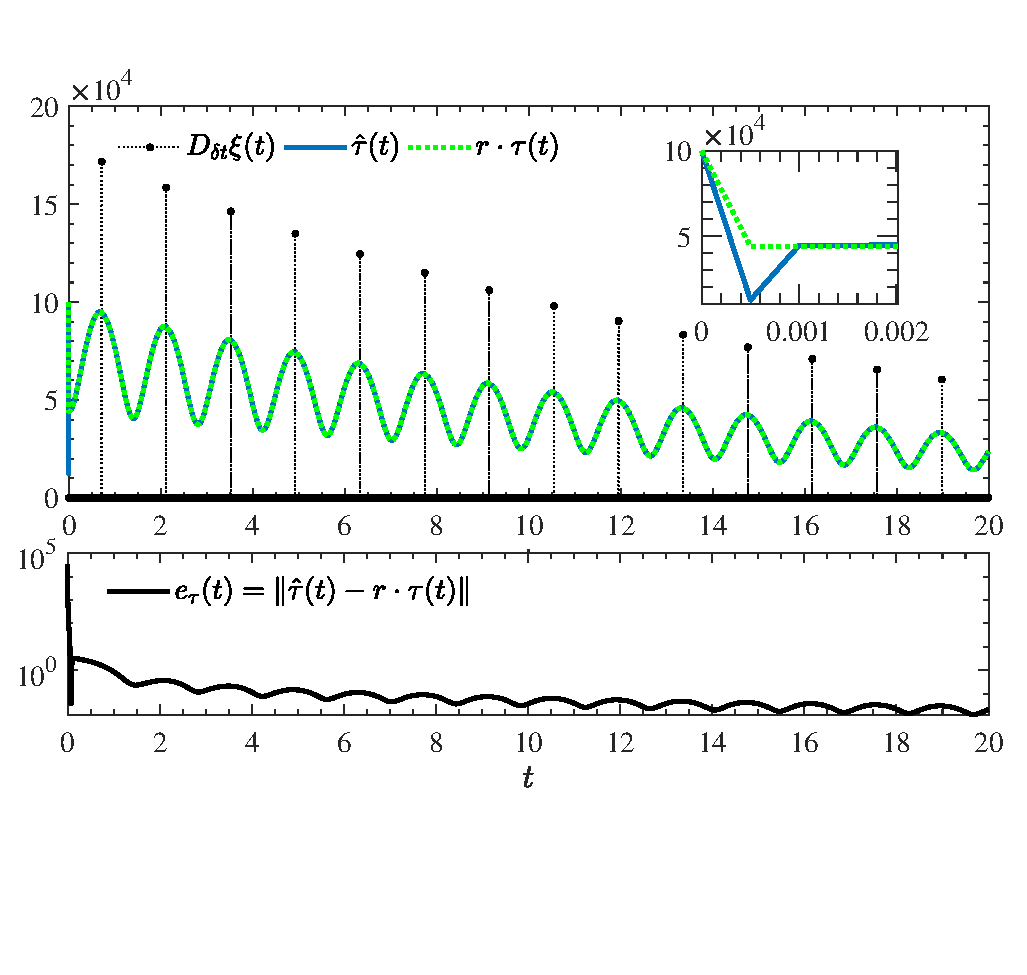
\includegraphics[trim={-10 0 0 0},scale=.75]{dderrnom}
	%\vspace*{-22mm}
	\caption[Nominal experiment: norm of the Euler derivative and estimated smoothness bound.]{Nominal experiment (no measurement noise). [Above] Norm of the Euler derivative $D_{\delta t}\x(t)$, (dotted black line and circe marker), estimated smoothness bound $\hat{\tau}(t)$ (blue solid line) and nominal smoothness bound $\tau(t)$ scaled by the arbitrary constant $r$. [Below] smoothness bound approximation error $e_{\tau}(t)$ (log scale).}
	\label{fig:dderrnom}
%vspace{-4.5mm}
\end{figure}
%
%
\begin{figure}[t!]
	%\vspace*{-18mm}
	\centering
	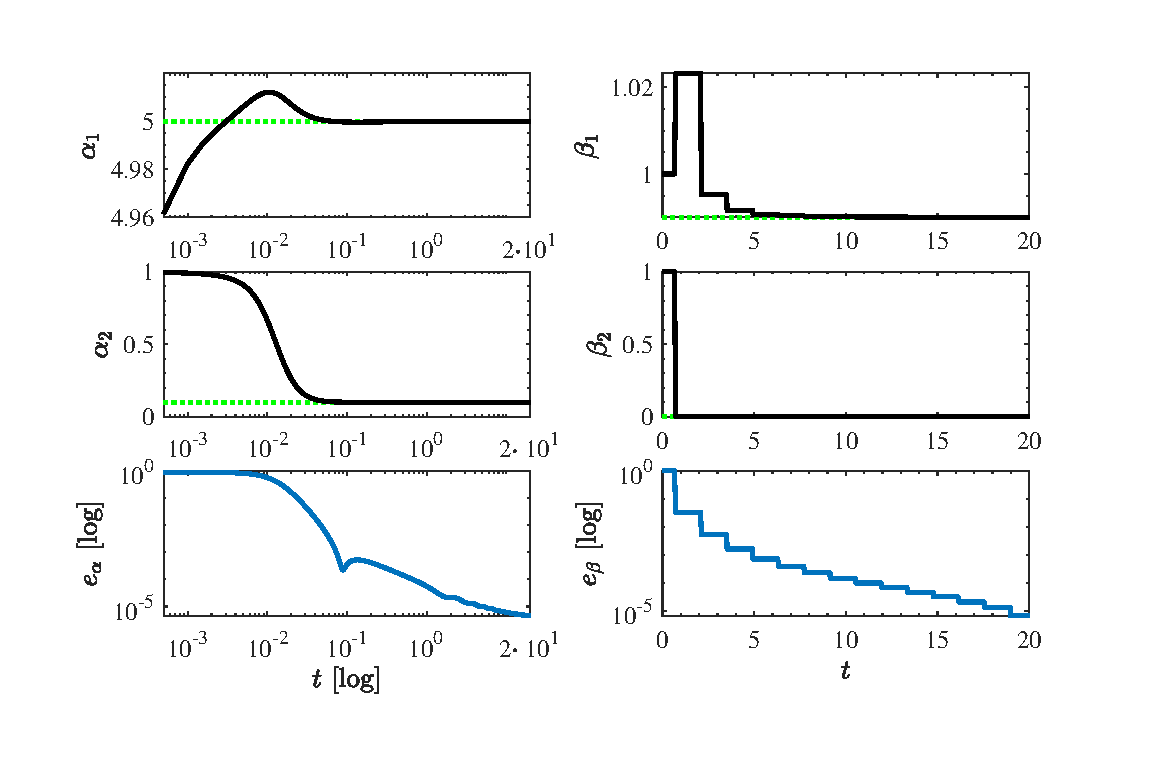
\includegraphics[trim={10 0 0 0},scale=.75]{parnom2}
	%\vspace*{-12mm}
	\caption[Nominal experiment: parameters estimation results.]{Nominal experiment (no measurement noise): parameters estimation results. [Left] Estimates of the parameters in $\bm{\alpha}$ and absolute estimation error $e_{\bm{\alpha}}(t)=\|\bm{\alpha}-\hat{\bm{\alpha}}(t)\|$ (below). [Right] Estimates of the parameters in $\bm{\beta}$ and absolute estimation error $e_{\bm{\beta}}(t)=\|\bm{\beta}-\hat{\bm{\beta}}(t)\|$ (below).}
	\label{fig:parnom}
	%\vspace{-7.5mm}
\end{figure}
%
\begin{figure}[t!]
	\centering
	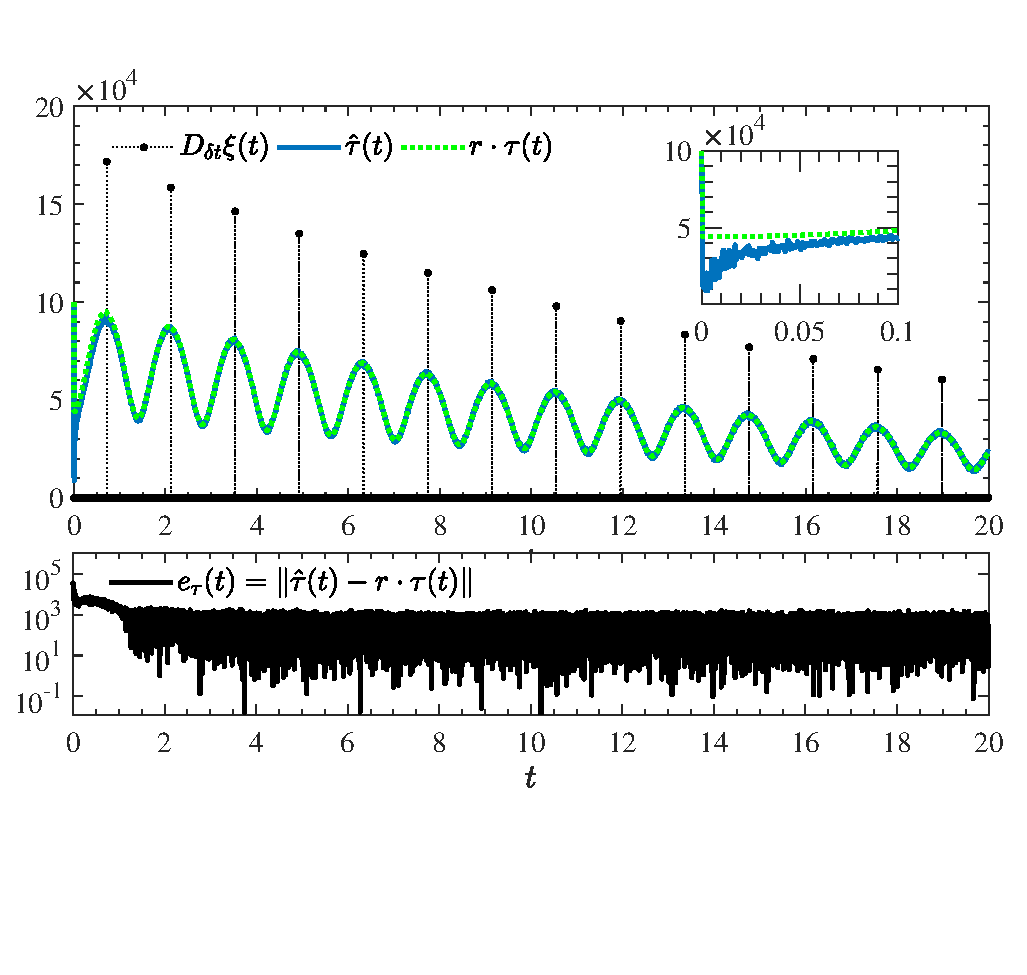
\includegraphics[trim={-10 0 0 0},scale=.75]{dderrnos2}
	%\vspace*{-22mm}
	\caption[Noisy experiment: norm of the Euler derivative and estimated smoothness bound.]{Noisy experiment (measurement noise standard deviation $\tilde{\sigma}_{\x}$=0.25). [Above] Norm of the Euler derivative $D_{\delta t}\x(t)$, (dotted black line and circle marker), estimated smoothness bound $\hat{\tau}(t)$ (blue solid line) and nominal smoothness bound $\tau(t)$ scaled by the arbitrary constant $r$. [Below] smoothness bound approximation error $e_{\tau}(t)$ (log scale).}
	\label{fig:dderrnos}
	%\vspace{-5mm}
\end{figure}
%
%
\begin{figure}[t!]
	\centering
	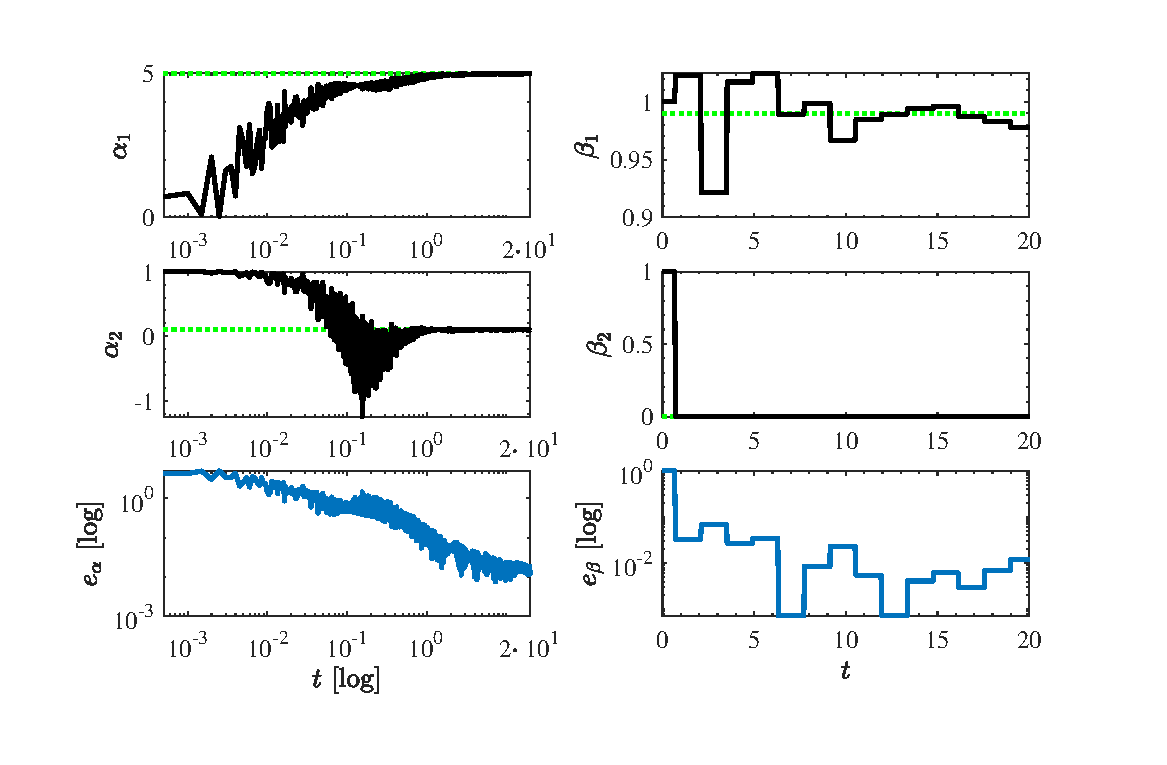
\includegraphics[trim={10 0 0 0},scale=0.75]{parnos}
	%\vspace*{-12mm}
	\caption[Noisy experiment: parameters estimation results.]{Noisy experiment (measurement noise standard deviation $\tilde{\sigma}_{\x}$=0.25): parameters estimation results. [Left] Estimates of the parameters in $\bm{\alpha}$ and absolute estimation error $e_{\bm{\alpha}}(t)=\|\bm{\alpha}-\hat{\bm{\alpha}}(t)\|$ (below). [Right] Estimates of the parameters in $\bm{\beta}$ and absolute estimation error $e_{\bm{\beta}}(t)=\|\bm{\beta}-\hat{\bm{\beta}}(t)\|$ (below).}
	\label{fig:parnos}
	%\vspace{-7mm}
\end{figure}

\clearpage
%%%%%%%%%%%%%%%%%%%%%%%%%%%%%%%%%%%%%%%%%%%%%%%%%%%%%%%%%%%%%%%%%%%%%%%%%%%%%%%%%%%%%%%%%%%
\section{Summary}\label{conc}
In this chapter, a new methodology for the identification of a class of hybrid dynamical systems, which evaluates the unknown parameters by employing a linear recursive estimator, has been proposed. The developed procedure is able to identify the state of the system and explicitly determine the flowing and jumping states. The method has been applied to a system falling in the category of hybrid port--Hamiltonian systems.
Here we have derived a systematic approach for the identification of hybrid dynamical systems, that to the best of authors' knowledge, is the first application of system identification methodologies to hybrid dynamical systems which can be analytically represented by Equation~\ref{eq:HS}.
Further development will include a more rigorous approach for the estimation of the smoothness bound without the need of any empirical coefficient, the exploration of alternative estimation schemes and a possible extension to the identification of \textit{hybrid inclusions}. Problems related to the non--convex approximation of the the flow and jump sets will also be regarded investigating new machine learning strategies.
%